% **************************************************************************************************************
% A Classic Thesis Style
% An Homage to The Elements of Typographic Style
%
% Copyright (C) 2012 Andr\'e Miede http://www.miede.de
%
% If you like the style then I would appreciate a postcard. My address 
% can be found in the file ClassicThesis.pdf. A collection of the 
% postcards I received so far is available online at 
% http://postcards.miede.de
%
% License:
% This program is free software; you can redistribute it and/or modify
% it under the terms of the GNU General Public License as published by
% the Free Software Foundation; either version 2 of the License, or
% (at your option) any later version.
%
% This program is distributed in the hope that it will be useful,
% but WITHOUT ANY WARRANTY; without even the implied warranty of
% MERCHANTABILITY or FITNESS FOR A PARTICULAR PURPOSE.  See the
% GNU General Public License for more details.
%
% You should have received a copy of the GNU General Public License
% along with this program; see the file COPYING.  If not, write to
% the Free Software Foundation, Inc., 59 Temple Place - Suite 330,
% Boston, MA 02111-1307, USA.
%
% **************************************************************************************************************
% Note:
%    * You must not use "u etc. in strings/commands that will be spaced out (use \"u or real umlauts instead)
%    * New enumeration (small caps): \begin{aenumerate} \end{aenumerate}
%    * For margin notes: \marginpar or \graffito{}
%    * Do not use bold fonts in this style, it is designed around them
%    * Use tables as in the examples
%    * See classicthesis-preamble.sty for useful commands
% **************************************************************************************************************
% To Do:
%		 * [high] Check this out: http://www.golatex.de/koma-script-warnung-in-verbindung-mit-listings-package-t2058.html
%    * [medium] mathbb in section-titles/chapter-titles => disappears somehow in headlines!!!
% **************************************************************************************************************

\documentclass[ twoside,openright,titlepage,numbers=noenddot,headinclude,%1headlines,% letterpaper a4paper
                footinclude=true,cleardoublepage=empty,abstractoff, % <--- obsolete, remove (todo)
                BCOR=5mm,paper=a4,fontsize=11pt,%11pt,a4paper,%
                ngerman,english,%
                ]{scrreprt}

%********************************************************************
% Note: Make all your adjustments in here
%*******************************************************
% ****************************************************************************************************
% classicthesis-config.tex 
% formerly known as loadpackages.sty, classicthesis-ldpkg.sty, and classicthesis-preamble.sty 
% Use it at the beginning of your ClassicThesis.tex, or as a LaTeX Preamble 
% in your ClassicThesis.{tex,lyx} with \input{classicthesis-config}
% ****************************************************************************************************  
% If you like the classicthesis, then I would appreciate a postcard. 
% My address can be found in the file ClassicThesis.pdf. A collection 
% of the postcards I received so far is available online at 
% http://postcards.miede.de
% ****************************************************************************************************

% ****************************************************************************************************
% 1. Configure classicthesis for your needs here, e.g., remove "drafting" below 
% in order to deactivate the time-stamp on the pages
% ****************************************************************************************************
\PassOptionsToPackage{drafting,eulerchapternumbers,listings,%drafting,%
				 pdfspacing,%floatperchapter,%linedheaders,%
				 subfig,beramono,eulermath,parts}{classicthesis}										
% ********************************************************************
% Available options for classicthesis.sty 
% (see ClassicThesis.pdf for more information):
% drafting
% parts nochapters linedheaders
% eulerchapternumbers beramono eulermath pdfspacing minionprospacing
% tocaligned dottedtoc manychapters
% listings floatperchapter subfig
% ********************************************************************

% ********************************************************************
% Triggers for this config
% ******************************************************************** 
\usepackage{ifthen}
\newboolean{enable-backrefs} % enable backrefs in the bibliography
\setboolean{enable-backrefs}{true} % true false
% ****************************************************************************************************


% ****************************************************************************************************
% 2. Personal data and user ad-hoc commands
% ****************************************************************************************************
\newcommand{\myTitle}{High-Performance Near-Time Processing of Bulk Data\xspace}
\newcommand{\mySubtitle}{A thesis submitted to the University of Plymouth in partial fulfilment for the degree of
doctor of philosophy\xspace}
\newcommand{\myDegree}{Master of Science\xspace}
\newcommand{\myName}{Martin Swientek\xspace}
\newcommand{\myProf}{Put name here\xspace}
\newcommand{\myOtherProf}{Put name here\xspace}
\newcommand{\mySupervisor}{Put name here\xspace}
\newcommand{\myFaculty}{School of Computing and Mathematics\xspace}
\newcommand{\myDepartment}{Put data here\xspace}
\newcommand{\myUni}{Plymouth University\xspace}
\newcommand{\myLocation}{Frankfurt\xspace}
\newcommand{\myTime}{September 2014\xspace}
\newcommand{\myVersion}{version 0.1\xspace}

% ********************************************************************
% Setup, finetuning, and useful commands
% ********************************************************************
\newcounter{dummy} % necessary for correct hyperlinks (to index, bib, etc.)
\newlength{\abcd} % for ab..z string length calculation
\providecommand{\mLyX}{L\kern-.1667em\lower.25em\hbox{Y}\kern-.125emX\@}
\newcommand{\ie}{i.\,e.}
\newcommand{\Ie}{I.\,e.}
\newcommand{\eg}{e.\,g.}
\newcommand{\Eg}{E.\,g.} 
% ****************************************************************************************************


% ****************************************************************************************************
% 3. Loading some handy packages
% ****************************************************************************************************
% ******************************************************************** 
% Packages with options that might require adjustments
% ******************************************************************** 
\PassOptionsToPackage{latin9}{inputenc}	% latin9 (ISO-8859-9) = latin1+"Euro sign"
 \usepackage{inputenc}				

\PassOptionsToPackage{english}{babel}   % change this to your language(s)
% Spanish languages need extra options in order to work with this template
%\PassOptionsToPackage{spanish,es-lcroman}{babel}
 \usepackage{babel}					

\PassOptionsToPackage{round}{natbib}
 \usepackage{natbib}
 
 \usepackage{multibib}
 \newcites{pub}{Publications}
 \nocitepub{*}

\PassOptionsToPackage{fleqn}{amsmath}		% math environments and more by the AMS 
 \usepackage{amsmath}

% ******************************************************************** 
% General useful packages
% ******************************************************************** 
\PassOptionsToPackage{T1}{fontenc} % T2A for cyrillics
	\usepackage{fontenc}     
\usepackage{textcomp} % fix warning with missing font shapes
\usepackage{scrhack} % fix warnings when using KOMA with listings package          
\usepackage{xspace} % to get the spacing after macros right  
\usepackage{mparhack} % get marginpar right
\usepackage{fixltx2e} % fixes some LaTeX stuff 
\PassOptionsToPackage{printonlyused,smaller}{acronym}
	\usepackage{acronym} % nice macros for handling all acronyms in the thesis
%\renewcommand*{\acsfont}[1]{\textssc{#1}} % for MinionPro
\renewcommand{\bflabel}[1]{{#1}\hfill} % fix the list of acronyms
\usepackage{enumerate}
% ****************************************************************************************************


% ****************************************************************************************************
% 4. Setup floats: tables, (sub)figures, and captions
% ****************************************************************************************************
\usepackage{booktabs}
%\usepackage{tabularx} % better tables
%	\setlength{\extrarowheight}{3pt} % increase table row height
%	\newcommand{\tableheadline}[1]{\multicolumn{1}{c}{\spacedlowsmallcaps{#1}}}
%	\renewcommand{\tabularxcolumn}[1]{>{\small}m{#1}}
\usepackage{ltablex}
	\keepXColumns
\newcommand{\myfloatalign}{\centering} % to be used with each float for alignment
\usepackage{caption}
\captionsetup{format=hang,font=small}
\usepackage{subfig}

\setlength{\extrarowheight}{3pt} % increase table row height
\newcommand{\tableheadline}[1]{\multicolumn{1}{c}{\spacedlowsmallcaps{#1}}}
\renewcommand{\tabularxcolumn}[1]{>{\small}m{#1}}

% fixes bug in ltablex which makes the table too narrow when using captions, see http://www.latex-community.org/forum/viewtopic.php?f=45&p=39951
\usepackage{etoolbox}% http://ctan.org/pkg/etoolbox
\makeatletter
\patchcmd{\TX@endtabularx}% <cmd>
  {\def\caption}% <search>
  {\def\caption{\caption@withoptargs\TX@caption}%
   \def\TX@caption##1##2}% <replace>
  {}{}% <success><failure>
\makeatother

% ****************************************************************************************************

% ****************************************************************************************************
% 5. Setup code listings
% ****************************************************************************************************
\usepackage{listings} 
%\lstset{emph={trueIndex,root},emphstyle=\color{BlueViolet}}%\underbar} % for special keywords
\lstset{language=[LaTeX]Tex,%C++,
    keywordstyle=\color{RoyalBlue},%\bfseries,
    basicstyle=\small\ttfamily,
    %identifierstyle=\color{NavyBlue},
    commentstyle=\color{Green}\ttfamily,
    stringstyle=\rmfamily,
    numbers=left,%left,%
    numberstyle=\scriptsize,%\tiny
    stepnumber=1,
    numbersep=8pt,
    showstringspaces=false,
    breaklines=true,
    frameround=ftff,
    frame=single,
    belowcaptionskip=.75\baselineskip,
	tabsize=2
    %frame=L
} 
% ****************************************************************************************************    		   


% ****************************************************************************************************
% 6. PDFLaTeX, hyperreferences and citation backreferences
% ****************************************************************************************************
% ********************************************************************
% Using PDFLaTeX
% ********************************************************************
\PassOptionsToPackage{pdftex,hyperfootnotes=false,pdfpagelabels}{hyperref}
	\usepackage{hyperref}  % backref linktocpage pagebackref
\pdfcompresslevel=9
\pdfadjustspacing=1 
\PassOptionsToPackage{pdftex}{graphicx}
	\usepackage{graphicx} 

\graphicspath{{./img/}}
\DeclareGraphicsExtensions{.pdf,.jpeg,.png}

% ********************************************************************
% Setup the style of the backrefs from the bibliography
% (translate the options to any language you use)
% ********************************************************************
\newcommand{\backrefnotcitedstring}{\relax}%(Not cited.)
\newcommand{\backrefcitedsinglestring}[1]{(Cited on page~#1.)}
\newcommand{\backrefcitedmultistring}[1]{(Cited on pages~#1.)}
\ifthenelse{\boolean{enable-backrefs}}%
{%
		\PassOptionsToPackage{hyperpageref}{backref}
		\usepackage{backref} % to be loaded after hyperref package 
		   \renewcommand{\backreftwosep}{ and~} % separate 2 pages
		   \renewcommand{\backreflastsep}{, and~} % separate last of longer list
		   \renewcommand*{\backref}[1]{}  % disable standard
		   \renewcommand*{\backrefalt}[4]{% detailed backref
		      \ifcase #1 %
		         \backrefnotcitedstring%
		      \or%
		         \backrefcitedsinglestring{#2}%
		      \else%
		         \backrefcitedmultistring{#2}%
		      \fi}%
}{\relax}    

% ********************************************************************
% Hyperreferences
% ********************************************************************
\hypersetup{%
    %draft,	% = no hyperlinking at all (useful in b/w printouts)
    colorlinks=true, linktocpage=true, pdfstartpage=3, pdfstartview=FitV,%
    % uncomment the following line if you want to have black links (e.g., for printing)
    %colorlinks=false, linktocpage=false, pdfborder={0 0 0}, pdfstartpage=3, pdfstartview=FitV,% 
    breaklinks=true, pdfpagemode=UseNone, pageanchor=true, pdfpagemode=UseOutlines,%
    plainpages=false, bookmarksnumbered, bookmarksopen=true, bookmarksopenlevel=1,%
    hypertexnames=true, pdfhighlight=/O,%nesting=true,%frenchlinks,%
    urlcolor=webbrown, linkcolor=RoyalBlue, citecolor=webgreen, %pagecolor=RoyalBlue,%
    %urlcolor=Black, linkcolor=Black, citecolor=Black, %pagecolor=Black,%
    pdftitle={\myTitle},%
    pdfauthor={\textcopyright\ \myName, \myUni, \myFaculty},%
    pdfsubject={},%
    pdfkeywords={},%
    pdfcreator={pdfLaTeX},%
    pdfproducer={LaTeX with hyperref and classicthesis}%
}   

% ********************************************************************
% Setup autoreferences
% ********************************************************************
% There are some issues regarding autorefnames
% http://www.ureader.de/msg/136221647.aspx
% http://www.tex.ac.uk/cgi-bin/texfaq2html?label=latexwords
% you have to redefine the makros for the 
% language you use, e.g., american, ngerman
% (as chosen when loading babel/AtBeginDocument)
% ********************************************************************
\makeatletter
\@ifpackageloaded{babel}%
    {%
       \addto\extrasamerican{%
					\renewcommand*{\figureautorefname}{Figure}%
					\renewcommand*{\tableautorefname}{Table}%
					\renewcommand*{\partautorefname}{Part}%
					\renewcommand*{\chapterautorefname}{Chapter}%
					\renewcommand*{\sectionautorefname}{Section}%
					\renewcommand*{\subsectionautorefname}{Section}%
					\renewcommand*{\subsubsectionautorefname}{Section}% 	
				}%
       \addto\extrasngerman{% 
					\renewcommand*{\paragraphautorefname}{Absatz}%
					\renewcommand*{\subparagraphautorefname}{Unterabsatz}%
					\renewcommand*{\footnoteautorefname}{Fu\"snote}%
					\renewcommand*{\FancyVerbLineautorefname}{Zeile}%
					\renewcommand*{\theoremautorefname}{Theorem}%
					\renewcommand*{\appendixautorefname}{Anhang}%
					\renewcommand*{\equationautorefname}{Gleichung}%        
					\renewcommand*{\itemautorefname}{Punkt}%
				}%	
			% Fix to getting autorefs for subfigures right (thanks to Belinda Vogt for changing the definition)
			\providecommand{\subfigureautorefname}{\figureautorefname}%  			
    }{\relax}
\makeatother


% ****************************************************************************************************
% 7. Last calls before the bar closes
% ****************************************************************************************************
% ********************************************************************
% Development Stuff
% ********************************************************************
\listfiles
%\PassOptionsToPackage{l2tabu,orthodox,abort}{nag}
%	\usepackage{nag}
%\PassOptionsToPackage{warning, all}{onlyamsmath}
%	\usepackage{onlyamsmath}

% ********************************************************************
% Last, but not least...
% ********************************************************************
\usepackage{classicthesis} 
% ****************************************************************************************************

\usepackage{todonotes}

% ****************************************************************************************************
% 8. Further adjustments (experimental)
% ****************************************************************************************************
% ********************************************************************
% Changing the text area
% ********************************************************************
%\linespread{1.05} % a bit more for Palatino
%\areaset[current]{312pt}{761pt} % 686 (factor 2.2) + 33 head + 42 head \the\footskip
%\setlength{\marginparwidth}{7em}%
%\setlength{\marginparsep}{2em}%

% ********************************************************************
% Using different fonts
% ********************************************************************
%\usepackage[oldstylenums]{kpfonts} % oldstyle notextcomp
%\usepackage[osf]{libertine}
%\usepackage{hfoldsty} % Computer Modern with osf
%\usepackage[light,condensed,math]{iwona}
%\renewcommand{\sfdefault}{iwona}
%\usepackage{lmodern} % <-- no osf support :-(
%\usepackage[urw-garamond]{mathdesign} <-- no osf support :-(
% ****************************************************************************************************


%********************************************************************
% Hyphenation
%*******************************************************
%\hyphenation{put special hyphenation here}

% ********************************************************************
% GO!GO!GO! MOVE IT!
%*******************************************************
\begin{document}
\frenchspacing
\raggedbottom
\selectlanguage{english} % american ngerman
%\renewcommand*{\bibname}{new name}
%\setbibpreamble{}
\pagenumbering{roman}
\pagestyle{plain}
%********************************************************************
% Frontmatter
%*******************************************************
%%!TEX root = ../thesis.tex
%*******************************************************
% Little Dirty Titlepage
%*******************************************************
\thispagestyle{empty}
%\pdfbookmark[1]{Titel}{title}
%*******************************************************
\begin{center}
    \spacedlowsmallcaps{\myName} \\ \medskip                        

    \begingroup
        \color{Maroon}\spacedallcaps{\myTitle} \\
    \endgroup
	\bigskip
	\center Doctor of Philosophy, \myTime
\end{center}        

%!TEX root = ../thesis.tex
%*******************************************************
% Titlepage
%*******************************************************
\begin{titlepage}
	% if you want the titlepage to be centered, uncomment and fine-tune the line below (KOMA classes environment)
	\begin{addmargin}[-1cm]{-3cm}
    \begin{center}
        \large  

        \hfill

        \vfill

        \begingroup
            \color{Maroon}\spacedallcaps{\myTitle} \\ \bigskip
        \endgroup

        \spacedlowsmallcaps{\myName}

        \vfill

        
\includegraphics[width=6cm]{plymouth_logo} \\ \bigskip
		
		\center A thesis submitted to the Plymouth University
		\center in partial fulfilment for the degree of \\ \medskip
		\spacedallcaps{Doctor of Philosophy} \\ \bigskip
        %\mySubtitle \\ \medskip   
        %\myDegree \\
        %\myDepartment \\                            
        %\myFaculty \\
        %\myUni \\ \bigskip

        \myTime\ -- \myVersion

        \vfill                      

    \end{center}  
  \end{addmargin}       
\end{titlepage}   
\thispagestyle{empty}

\hfill

\vfill

This copy of the thesis has been supplied on condition that anyone who consults it is understood to recognise that its copyright rests with its author and that no quotation from the thesis and no information derived from it may be published without the author's prior consent.
\\\\
\noindent\myName: \textit{\myTitle,} %\mySubtitle, %\myDegree, 
\textcopyright\ \myTime

%\bigskip
%
%\noindent\spacedlowsmallcaps{Supervisors}: \\
%\myProf \\
%\myOtherProf \\ 
%\mySupervisor
%
%\medskip
%
%\noindent\spacedlowsmallcaps{Location}: \\
%\myLocation
%
%\medskip
%
%\noindent\spacedlowsmallcaps{Time Frame}: \\
%\myTime

%\cleardoublepage%!TEX root = ../thesis.tex
%*******************************************************
% Dedication
%*******************************************************
\thispagestyle{empty}
%\phantomsection 
\refstepcounter{dummy}
\pdfbookmark[1]{Dedication}{Dedication}

\vspace*{3cm}

\begin{center}
    \emph{Ohana} means family. \\
    Family means nobody gets left behind, or forgotten. \\ \medskip
    --- Lilo \& Stitch    
\end{center}

\medskip

\begin{center}
    Dedicated to the loving memory of Rudolf Miede. \\ \smallskip
    1939\,--\,2005
\end{center}
%\cleardoublepage\include{FrontBackmatter/Foreword}
%\cleardoublepage%!TEX root = ../thesis.tex
%*******************************************************
% Abstract
%*******************************************************
%\renewcommand{\abstractname}{Abstract}
\pdfbookmark[1]{Abstract}{Abstract}
\begingroup
\let\clearpage\relax
\let\cleardoublepage\relax
\let\cleardoublepage\relax

\chapter*{Abstract}
\begin{center}
\spacedallcaps{\myTitle}\\ \medskip
\spacedlowsmallcaps{\myName} \bigskip
\end{center}
\lipsum[1-3]

\vfill
\endgroup			

\vfill
%\cleardoublepage%!TEX root = ../thesis.tex
%*******************************************************
% Acknowledgments
%*******************************************************
\pdfbookmark[1]{Acknowledgments}{acknowledgments}

%\begin{flushright}{\slshape    
%    We have seen that computer programming is an art, \\ 
%    because it applies accumulated knowledge to the world, \\ 
%    because it requires skill and ingenuity, and especially \\
%    because it produces objects of beauty.} \\ \medskip
%    --- \defcitealias{knuth:1974}{Donald E. Knuth}\citetalias{knuth:1974} \citep{knuth:1974}
%\end{flushright}

\bigskip

\begingroup
\let\clearpage\relax
\let\cleardoublepage\relax
\let\cleardoublepage\relax
\chapter*{Acknowledgments}
\lipsum[1]


\endgroup




%\cleardoublepage%!TEX root = ../thesis.tex
%*******************************************************
% Declaration
%*******************************************************
\refstepcounter{dummy}
\pdfbookmark[0]{Declaration}{declaration}
\chapter*{Declaration}
\thispagestyle{empty}
Put your declaration here.
\bigskip
 
\noindent\textit{\myLocation, \myTime}

\smallskip

\begin{flushright}
    \begin{tabular}{m{5cm}}
        \\ \hline
        \centering\myName \\
    \end{tabular}
\end{flushright}

\pagestyle{scrheadings}
\cleardoublepage%*******************************************************
% Table of Contents
%*******************************************************
%\phantomsection
\refstepcounter{dummy}
\pdfbookmark[1]{\contentsname}{tableofcontents}
\setcounter{tocdepth}{2} % <-- 2 includes up to subsections in the ToC
\setcounter{secnumdepth}{3} % <-- 3 numbers up to subsubsections
\manualmark
\markboth{\spacedlowsmallcaps{\contentsname}}{\spacedlowsmallcaps{\contentsname}}
\tableofcontents 
\automark[section]{chapter}
\renewcommand{\chaptermark}[1]{\markboth{\spacedlowsmallcaps{#1}}{\spacedlowsmallcaps{#1}}}
\renewcommand{\sectionmark}[1]{\markright{\thesection\enspace\spacedlowsmallcaps{#1}}}
\renewcommand\thepart{\Roman{part}}
%*******************************************************
% List of Figures and of the Tables
%*******************************************************
\clearpage

\begingroup 
    \let\clearpage\relax
    \let\cleardoublepage\relax
    \let\cleardoublepage\relax
    %*******************************************************
    % List of Figures
    %*******************************************************    
    %\phantomsection 
    \refstepcounter{dummy}
    %\addcontentsline{toc}{chapter}{\listfigurename}
    \pdfbookmark[1]{\listfigurename}{lof}
    \listoffigures

    \vspace*{8ex}

    %*******************************************************
    % List of Tables
    %*******************************************************
    %\phantomsection 
    \refstepcounter{dummy}
    %\addcontentsline{toc}{chapter}{\listtablename}
    \pdfbookmark[1]{\listtablename}{lot}
    \listoftables
        
    \vspace*{8ex}
%   \newpage
    
    %*******************************************************
    % List of Listings
    %*******************************************************      
	  %\phantomsection 
    \refstepcounter{dummy}
    %\addcontentsline{toc}{chapter}{\lstlistlistingname}
    \pdfbookmark[1]{\lstlistlistingname}{lol}
    \lstlistoflistings 

    \vspace*{8ex}
       
    %*******************************************************
    % Acronyms
    %*******************************************************
    %\phantomsection 
    \refstepcounter{dummy}
    \pdfbookmark[1]{Acronyms}{acronyms}
    \markboth{\spacedlowsmallcaps{Acronyms}}{\spacedlowsmallcaps{Acronyms}}
    \chapter*{Acronyms}
    \begin{acronym}[JAXB]
		\acro{API}{Application Programming Interface}
		\acro{CDR}{Call Detail Records}
		\acro{DB}{Database}
		\acro{ETL}{Extract, Transform, Load}
		\acro{ESB}{Enterprise Service Busx}
		\acro{NCDR}{Normalized Call Detail Records}
		\acro{FIFO}{First In, First Out}
		\acro{FTP}{File Transfer Protocol}
		\acro{JAXB}{Java Architecture for XML Binding}
        \acro{JMS}{Java Messaging Service}
		\acro{JPA}{Java Persistence API}
		\acro{NTP}{Network Time Protocol}
		\acro{ORM}{Object-relational mapping}
		\acro{PTP}{Precision Time Protocol}
		\acro{SLA}{Service Level Agreements}
        \acro{SOA}{Service Oriented Architecture}
    \end{acronym}                     
\endgroup

\cleardoublepage
%********************************************************************
% Mainmatter
%*******************************************************
\pagenumbering{arabic}
%\setcounter{page}{90}
% use \cleardoublepage here to avoid problems with pdfbookmark
\cleardoublepage
\part{Field of Research}
\cleardoublepage%!TEX root = ../thesis.tex
%******************************************************************************
\chapter{Introduction}\label{ch:introduction}
%******************************************************************************

Enterprise Systems like customer-billing systems or financial transaction systems are required to process large volumes of data in a fixed period of time. For example, a billing system for a large telecommunication provider has to process more than 1 million bills per day.
Those systems are increasingly required to also provide near-time processing of data to support new service offerings.

Traditionally, enterprise systems for bulk data processing are implemented as batch processing systems \citep{Fleck:1999aa}. Batch processing delivers high throughput but cannot provide near-time processing of data, that is the end-to-end latency of such a system is high. End-to-end latency refers to the period of time that it takes for a business process, implemented by multiple subsystems, to process a single business event.  For example, consider the following billing system of telecommunications provider:
\begin{itemize}
	\item Customers are billed once per month
	\item Customers are partitioned in 30 billing groups
	\item The billing system processes 1 billing group per day, running 24h under full load.
\end{itemize}
In this case, the mean time for a call event to be billed by the billing system is 1/2 month. That is, the mean end-to-end latency of this system is 1/2 month.

A lower end-to-end latency can be achieved by using single-event processing, for example by utilizing a message-oriented middleware for the integration of the services that form the enterprise system. While this approach is able to deliver near-time processing, it is hardly capable for bulk data processing due to the additional communication overhead for each processed message. Therefore, message-based processing is usually not considered for building a system for bulk data processing requiring high throughput.

The processing type is usually a fixed property of an enterprise system that is decided when the architecture of the system is designed, prior to implementing the system. This choice depends on the non-functional requirements of the system. These requirements are not fixed and can change during the lifespan of a system, either anticipated or not anticipated.

Additionally, enterprise systems often need to handle load peaks that occur infrequently. For example, think of a billing system with moderate load over most of the time, but there are certain events with very high load such as New Year's Eve. Most of the time, a low end-to-end latency of the system is preferable when the system faces moderate load. During the peak load, it is more important that the system can handle the load at all. A low end-to-end latency is not as important as an optimized maximum throughput in this situation.

\section{Aims and Objectives of the Research}\label{sec:research_objectives}
This research project aims to find a solution for the following problem:
\begin{quote}
\textbf{How to achieve high-performance near-time processing of bulk data?}
\end{quote}
To approach this problems, the research project has the following key objectives:
\begin{enumerate}[A.]
	\item Performance evaluation of batch and messaging systems regarding throughput and latency.
	\item Development of a concept for an adaptive middleware that delivers low latency while providing high throughput.
	\item Implementation of a research prototype used for demonstrating the practicability of the concept.
	\item Specification and conduction of appropriate performance tests to evaluate the developed approach.
	\item Development of a conceptional framework containing guidelines and rules for the practitioner how to implement an enterprise system based on the adaptive middleware for near-time processing of bulk data.
\end{enumerate}

\section{Research Methodology}

\section{Contributions}\label{sec:contributions}

\begin{itemize}
	\item Performance evaluation of batch and messaging systems regarding throughput and latency
	\item Concept and prototype implementation of an adaptive middleware 
	\item Conceptional Framework
\end{itemize}

\section{Outline of the Thesis}\label{sec:thesis_outline}

\begin{enumerate}
	\item Introduction
	\item Background
	\item Related Work
	\item Performance Evaluation of Batch and Message-based Systems
	\item An Adaptive Middleware for Near-Time Processing of Bulk Data
	\item A Conceptual Framework For Feedback-Controlled Bulk Data Processing Systems
	\item Conclusion
\end{enumerate}
\cleardoublepage%!TEX root = ../thesis.tex
%******************************************************************************
\chapter{Background}\label{ch:background}
%******************************************************************************

This chapter further defines the context of the conducted research and introduces core concepts and terms that are used throughout the thesis. It starts with an introduction of batch and message-based processing. The terms latency and throughput are defined and their relationship is analyzed. 
The term \ac{SOA} is a briefly introduced, followed by a short description of \ac{ESB} middleware technology. Additionally, it describes \acp{EIP}, that can be used to improve the performance of messaging systems. The chapter describes performance issues of an \ac{SOA} middleware and discusses common approaches for performance optimizations of such a middleware.

\section{Batch Processing}\label{sec:batch_processing}
The traditional operation paradigm of a system for bulk data processing is batch processing (see Figure \ref{fig:batch_processing}). A batch processing system is an application that processes bulk data without user interaction. Input and output data is usually organised in records using a file- or database-based interface. In the case of a file-based interface, the application reads a record from the input file, processes it and writes the record to the output file.
\begin{figure}[htbp]
	\centering
	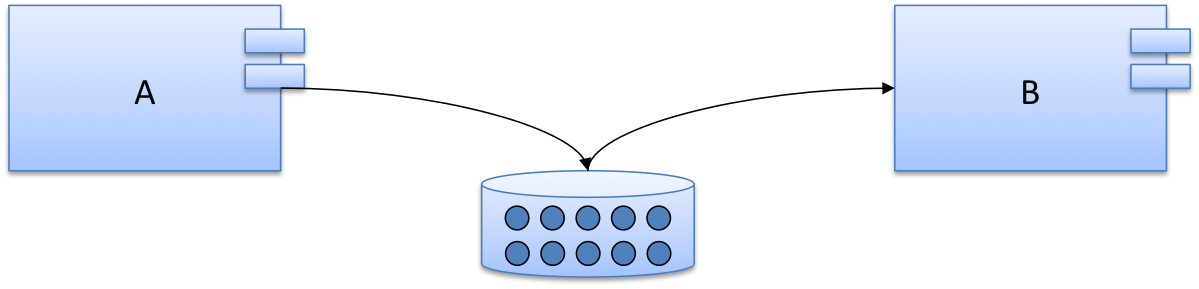
\includegraphics[width=\columnwidth]{batch}
	\caption{Batch processing}
	\label{fig:batch_processing}
\end{figure}

A batch processing system exhibits the following key characteristics:
\begin{itemize}
	\item \textbf{Bulk processing of data}\\
	A Batch processing system processes several gigabytes of data in a single run thus providing a high throughput. Multiple systems are running in parallel, controlled by a job scheduler to speed up processing. The data is usually partitioned and sorted by certain criteria for optimized processing. For example, if a batch only contains data for a specific product, the system can pre-load all necessary reference data from the database to speed up the processing.
	\item \textbf{No user interaction}\\
	There is no user interaction needed for the processing of data. It is impossible due to the amount of data being processed.
	\item \textbf{File- or database-based interfaces}\\
	Input data is read from the file system or a database. Output data is also written to files on the file system or a database. Files are transferred to the consuming systems through FTP by specific jobs.
	\item \textbf{Operation within a limited timeframe}\\
	A batch processing system often has to deliver its results in a limited timeframe due to \ac{SLA} with consuming systems. This timeframe is commonly called the batch window.
	\item \textbf{Offline handling of errors}\\
	Erroneous records are stored to a specific persistent memory (file or database) during operation and are processed afterwards.
\end{itemize}
Applications that are usually implemented as batch processing systems are billing systems for telecommunication companies used for mediating, rating and billing of call events.

\subsection{Integration Styles}
Batch processing systems use different styles to integrate with their outside environment or the integration of their subcomponents, with file-based and database-based integration being the most common. A combination of both styles is also possible.

\begin{itemize}
	\item \textbf{File transfer}\\
	With a file-based integration, the batch system or its subcomponents read the data from the input file, processes it and writes the output to the output file.
The file is transported to the next (sub-) system using \ac{FTP}, \ac{SCP} or other protocols for file transfer. The transfer is usually started by a specific job. Alternatively, a shared filesystem, such as \ac{NFS} can be used. The system also needs to be notified when new input data is ready for processing, for example by actively monitoring a certain folder or by getting notified from the previous system in the processing chain.
	\item \textbf{Shared database}\\
	The batch system or its subcomponents read and write the input and output data to a database, which is shared among all (sub-) systems. 
\end{itemize}

\subsection{Batch Performance Optimisations}

A batch-oriented system can be highly optimized for high throughput:

\begin{itemize}
	\item \textbf{Data formats}\\
	Using optimized data formats such as binary formats or \ac{CSV} data formats, that are optimized for reading and writing. Additionally, input and output data can be compressed to reduce data transfer times.
	\item \textbf{Database transactions}\\
	Database transactions introduce a major performance cost when processing large volumes of data. Batch processing system therefore minimize the amount of transactions by encapsulating a whole batch in one transaction, not every single record.
	\item \textbf{Database design and technologies}\\
	The database access can optimized by using pre-computed views especially designed for batch processing, such flattenend relations.
	Additionally, other database concepts than relational databases like No-SQL or in-memory databases can be used to further optimize the persistence layer.
	\item \textbf{Optimization depending on data semantics or technical properties}\\
	When data is processed in batches and is sorted accordingly to some business or technical rules, the processing algorithm can easily make assumptions about the data and optimize its processing. For example, when a batch only contains flat rate \ac{CDR} or \ac{CDR} of a specific product or customer segment, the corresponding reference data can be pre-loaded.
	\item \textbf{Caching}\\
	Often used data such as reference data, for example products and tariffs in case of a billing system, can also be cached in memory, prior to processing.
\end{itemize}

\subsection{Demarcation to Big Data}
Big Data is a term that generally describes large amounts of data, that is too big to process with traditional data processing applications, such as \ac{SQL}-based databases. In the context of \emph{Big Data}, a data processing application is defined as a system, that ``answers questions based on information that was acquired in the past'' (cf. \cite{Merz:2014aa}). These systems are commonly used in the realm of analytics to get better insights on the business. 

Technologies for implementing such as a system, like Apache Hadoop \citep{apachehadoop} are not considered for near-time processing of data, due to their high latency (cf. \cite{Merz:2014aa}).

\section{Message-based Processing}\label{sec:message_processing}
Messaging facilitates the integration of heterogeneous applications using asynchronous communication. Applications are communicating with each other by sending messages (see Figure \ref{fig:message_based_processing}). A messaging server or message-oriented middleware handles the asynchronous exchange of messages including an appropriate transaction control \citep{conrad2006enterprise}.

In the context of this thesis, messaging is a mean to implement single-event processing.

\begin{figure}[htbp]
	\centering
	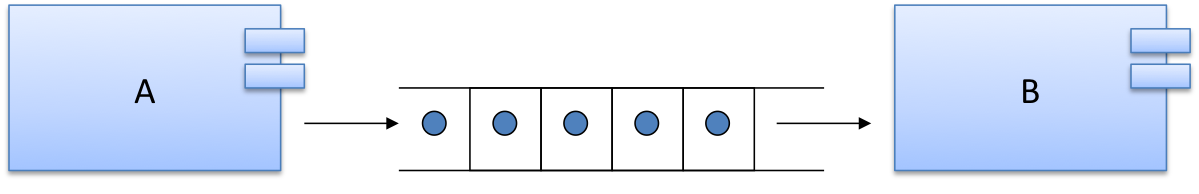
\includegraphics[width=\columnwidth]{esb}
	\caption{Message-based processing}
	\label{fig:message_based_processing}
\end{figure}

\cite{Hohpe:2003fk} describe the following basic messaging concepts:
\begin{itemize}
	\item \textbf{Channels}\\
	Messages are transmitted through a channel. A channel connects a message sender to a message receiver.
	\item \textbf{Messages}\\
	A message is packet of data that is transmitted through a channel. The message sender breaks the data into messages and sends them on a channel. The message receiver in turn reads the messages from the channel and extracts the data from them.
	\item \textbf{Pipes and Filters}\\
	A message may pass through several processing steps before it reaches its final destination. Multiple processing steps are chained together using a pipes and filters architecture.
	\item \textbf{Routing}\\
	A message may have to go through multiple channels before it reaches its destination. A message router acts as a filter and is capable of routing a message to the next channel or to another message router.
	\item \textbf{Transformation}\\
	A message can be transformed by a message translator if the message sender and receiver do not agree on the format for the same conceptual data.
	\item \textbf{Endpoints}\\
	A message endpoint is a software layer that connects arbitrary applications to the messaging system.
\end{itemize}

\subsection{Messaging Concepts}

There are two types of message channels (cf. \cite{Hohpe:2003fk}):

\begin{itemize}
	\item \textbf{Point To Point}\\
	A \emph{Point To Point} channel is used to send messages to only one receiver. The messaging system ensures that a message is consumed only once. A \emph{Point To Point} can also have multiple competing consumers, in this way, messages can be load-balanced among multiple consumers to scale the processing system. 
	\item \textbf{Publish-Subscribe}\\
	A \emph{Publish-Subscribe} channel is used to broadcast a message to multiple receivers. When a message is sent to input channel of the \emph{Publish-Subsriber} channel, the messaging system copies the message to multiple output channels, one chanel for each receiver. Each subscriber gets the message only once.
\end{itemize}

The adaptive middleware presented in this thesis only uses \emph{Point To Point} message channels with competing consumers.

Additionally, there are two important concepts for the transmission of messages (cf. \cite{Hohpe:2003fk}):

\begin{itemize}
	\item \textbf{Send and forget}\\
	The sending system sends the message to the message channel. The messaging system transmits the message in the background, the sender does not have to wait until the receiving system reads the message.
	\item \textbf{Store and forward}\\
	When the sending system sends the message to the message channel, the messaging system stores the message on the system of the sender and forwards it to the receiver by storing it to the receiving system. This can be repeated until the receiver receives the message.
\end{itemize}

In the context of this thesis, only \emph{Send and forget} is considered.
\\\\
Message-based systems are able to provide near-time processing of data due to their lower latency compared with batch processing systems. The advantage of a lower latency comes with a performance cost in regard to a lower throughput because of the additional overhead for each processed message. Every message needs amongst others to be serialised and deserialised, mapped between different protocols and routed to the appropriate receiving system. Section \ref{sec:ch02_performance_issues} contains a detailed discussion of performance issues of message-based service-oriented middleware.

\section{Latency vs. Throughput}\label{sec:ch2_latency_throughput}
Throughput and latency are performance metrics of a system. The following definitions of throughput and latency are used in this thesis:
\begin{itemize}
	\item \textbf{Maximum Throughput}\\
	The number of events the system is able to process in a fixed timeframe.
 	\item \textbf{Ent-to-end Latency}\\
	The period of time between the occurrence of an event and its processing. End-to-end latency refers to the total latency of a complete business process implemented by multiple subsystems. The remainder of this paper focusses on end-to-end latency using the general term latency as an abbreviation.
\end{itemize}
\subsubsection{Batch processing}
A business process, such as billing, implemented by a system using batch processing exhibits a high end-to-end latency. For example, consider the following billing system:
\begin{itemize}
	\item Customers are billed once per month
	\item Customers are partitioned in 30 billing groups
	\item The billing system processes 1 billing group per day, running 24h under full load.
\end{itemize}

In this case, the mean time for a call event to be billed by the billing system is $1/2$ month. That is, the mean end-to-end latency of this system is $1/2$ month.

\begin{figure}[h!]
	\centering
	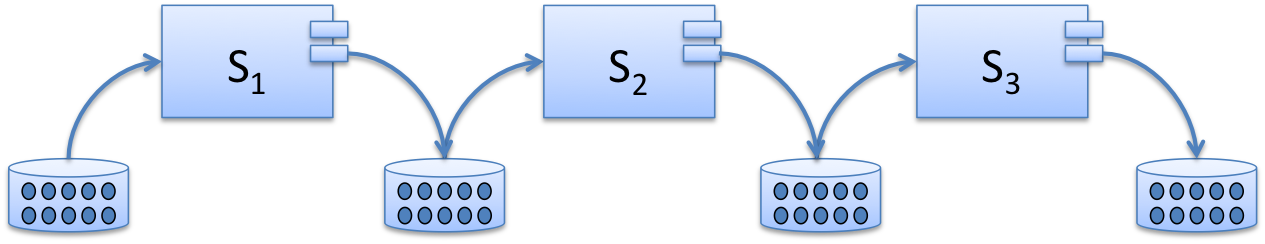
\includegraphics[width=\columnwidth]{latency_throughput1}
	\caption{Batch processing system comprised of three subsystems}
	\label{fig:batch_processing_latency}
\end{figure}

Assuming the system $S_{Batch}$ which is comprised of $N$ subsystems $S_1$, $S_2$, \ldots, $S_N$ (see Figure \ref{fig:batch_processing_latency} for an example with $N=3$):
\begin{displaymath}
S_{Batch} = \{S_1, S_2, \ldots, S_N\}
\end{displaymath}
The subsystem $S_i$ reads its input data from the database $DB_i$ in one chunk, processes it and writes the output to the database $DB_{i+1}$. When $S_i$ has finished the processing, the next subsystem $S_{i+1}$ reads the input data from $DB_{i+1}$, processes it and writes the output to $DB_{i+2}$, which in turn is read and processed from subsystem $S_{i+3}$ and so on.

The latency $L_{E_{S_{Batch}}}$ of a single event processed by the system $S_{Batch}$ is determined by the total processing time $PT_{S_{Batch}}$, which is the sum of the processing time $PT_i$ of each subsystem $S_i$:
\begin{displaymath}
L_{E_{S_{Batch}}} = PT_{S_{Batch}} = \sum_{i=1}^N PT_i
\end{displaymath}
where $N$ is the number of subsystems.

The processing time $PT_i$ of the subsystem $S_i$ is the sum of the processing time of each event $PT_{E_{j}}$ and the additional processing overhead $OH_i$, which includes the time spent for reading and writing the data, opening and closing transactions, etc:
\begin{displaymath}
PT_i = \left(\sum_{j=1}^M PT_{E_{j}}\right) + OH_i
\end{displaymath}
where $M$ is the number of events.

To allow for near-time processing, it is necessary to decrease the latency $L_{E_S}$ of a single event. This is can be achieved by using message-based processing instead of batch processing.

\subsubsection{Message-based processing}
The subsystem $S_i$ of a message-based system $S_{Message}$ reads a single event from its input message queue $MQ_i$, processes it and writes it to the output message queue $MQ_{i+1}$. As soon as the event is written to the message queue $MQ_{i+1}$, it is read by the subsystem $S_{i+1}$, which processes the event and writes to the message queue $MQ{i+2}$ and so on (see Figure \ref{fig:message_based_latency}).

The latency $L_{E_{S_{Message}}}$ of a single event processed by the system $S_{Message}$ is determined by the total processing time $PT_{E_{S_{Message}}}$ of this event, which is the sum of the processing time $PT_{E_i}$ and the processing overhead $OH_{E_{i}}$ for the event of each subsystem:
\begin{displaymath}
L_{E_{S_{Message}}} = PT_{E_{S_{Message}}} = \sum_{i+1}^N (PT_{E_i} + OH_{E_i})	
\end{displaymath}
where $N$ is the number of subsystems. Please note that the wait time of the event is assumed to be 0 for simplification.

The processing overhead $OH_{E_i}$ includes amongst others the time spent for unmarshalling and marshalling, protocol mapping and opening and closing transactions, which is done for every processed event.

\begin{figure}[h!]
	\centering
	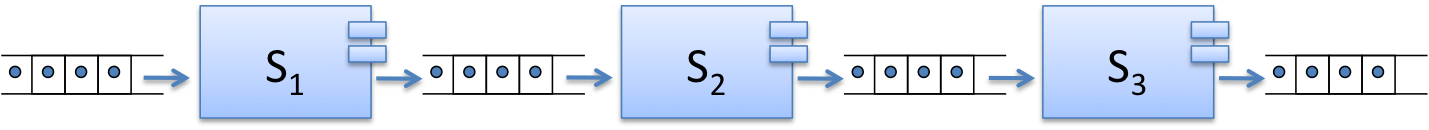
\includegraphics[width=\columnwidth]{latency_throughput2}
	\caption{Message-based system comprised of three subsystems}
	\label{fig:message_based_latency}
\end{figure}

Since the processing time $PT_{E_{S_{Message}}}$ of a single event is much shorter than the total processing time $PT_{S_{Batch}}$ of all events, the latency $L_{E_{S_{Message}}}$ of a single event using a message-based system is much smaller than the latency $L_{E_{S_{Batch}}}$ of a single event processed by a batch-processing system.
\begin{displaymath}
PT_{E_{S_{Message}}} < PT_{S_{Batch}} \Rightarrow L_{E_{S_{Message}}} < L_{E_{S_{Batch}}}
\end{displaymath}

Message-based processing adds an overhead to each processed event in contrast to batch processing, which adds a single overhead to each processing cycle. Hence, the accumulated total processing overhead $OH_{S_{Message}}$ of a message-based system $S_{Message}$ for processing $m$ events is larger than the total processing overhead of a batch processing system:
\begin{displaymath}
OH_{S_{Message}} = \sum_{i=1}^n OH_{E_i} * m > OH_{S_{Batch}} = \sum_{i=1}^n OH_i
\end{displaymath}
A message-based system, while having a lower end-to-end latency, is not able to process the same amount of events in the same time as a batch processing system and therefore cannot provide the same maximum throughput.

\begin{figure}[h!]
	\centering
	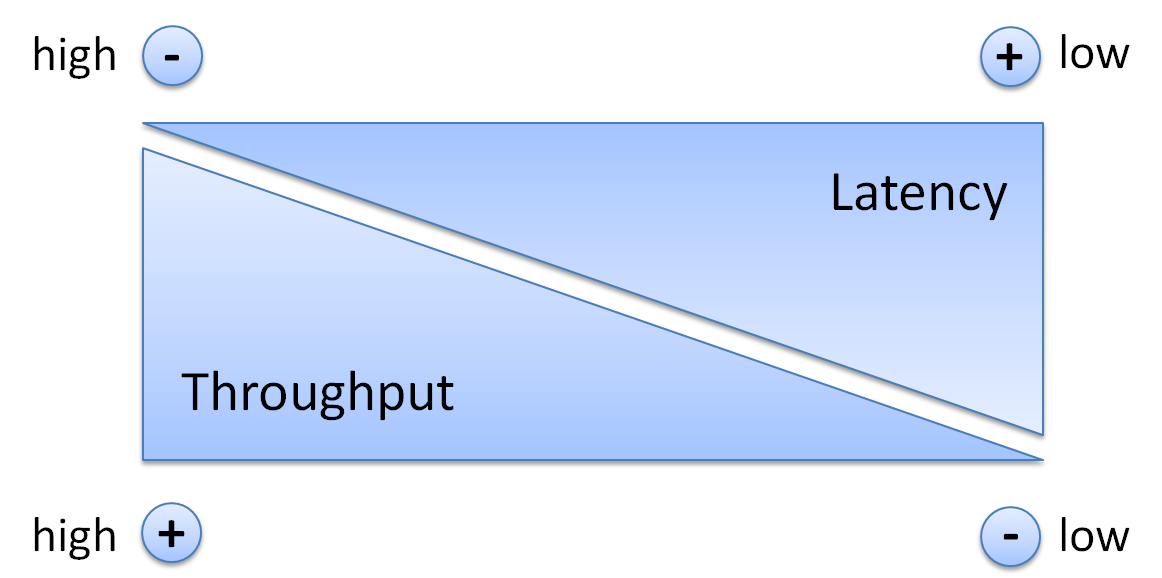
\includegraphics[width=\columnwidth]{latency_vs_throughput}
	\caption{Latency and throughput are opposed to each other}
	\label{fig:latency_vs_throughput}
\end{figure}

From this follows that latency and throughput are opposed to each other (see Figure \ref{fig:latency_vs_throughput}). High throughput, as provided by batch processing, leads to high latency, which impedes near-time processing. On the other hand, low latency, as provided by a message-based system, cannot provide the throughput needed for bulk data processing because of the additional overhead for each processed event.

\section{Service-Oriented Architecture}
\ac{SOA} is an architectural pattern to build application landscapes from single business components. These business components are loosely coupled by providing their functionality in form of services.  A service represents an abstract business view of the functionality and hides all implementation details of the component providing the service. The definition of a service acts as a contract between the service provider and the service consumer. Services are called using a unified mechanism, which provides a plattform independent connection of the business components while hiding all the technical details of the communication. The calling mechanism also includes the discovery of the appropriate service
\citep{Richter:2005ci}.

By separating the technical from the business aspects, SOA aims for a higher level of flexibility of enterprise applications.
\section{Enterprise Service Bus}
An \ac{ESB} is an integration platform that combines messaging, web services, data transformation and intelligent routing \citep{Schulte:2002mz}.
Table \ref{tab:char_esb} shows the main characteristics of an ESB \citep{Chappell:2004jo}.
\begin{table}[htbp]
	\centering
	\begin{tabular}{|p{0.3\textwidth}|p{0.6\textwidth}|}
		\hline
		Pervasiveness & An ESB supports multiple protocols and client technologies. It can span an entire organisation including its business partners. \\ \hline
		Highly distributed & An ESB integrates loosely coupled application components that form a highly distributed network. \\ \hline
		Selective deployment of integration components & The services of an ESB are independent of each other and can be separately deployed. \\ \hline
		Security and reliability & An ESB provides reliable messaging, transactional integrity and secure authentication. \\ \hline
		Orchestration and process flow & An ESB supports the orchestration of application components controlled by message metadata or an orchestration language like WS-BPEL. \\ \hline
		Autonomous yet federated managed environment & Different departments can still separately manage an ESB that spans the whole organisation. \\ \hline
		Incremental adoption & The adoption of an ESB can be incremental one project after another. \\ \hline
		XML support & XML is the native data format of an ESB. \\ \hline
		Real-time insight & An ESB provides real-time throughput of data by the use of its underlying message-oriented middleware and thus decreases latency. \\
		\hline
	\end{tabular}
	\caption{Main characteristics of an ESB \citep{Chappell:2004jo}}
	\label{tab:char_esb}
\end{table}
All application components and integration services that are connected to the ESB are viewed as abstract service endpoints. Abstract endpoints are logical abstractions of services that are plugged into the ESB and are all equal participants \citep{Chappell:2004jo}. An abstract endpoint can represent a whole application package such as a CRM or ERP system, a small web service or an integration service of the ESB such as a monitoring, logging or transformation service. As integration platform the ESB supports various types of connections for the service endpoints. These can be SOAP, HTTP, FTP, JMS or other programming APIs for C, C++, C\#, etc. It is often stated that ``if you can't bring the application to the bus, bring the bus to the application'' \citep{Chappell:2004jo}.

The backbone of the ESB is a message-oriented middleware (MOM), which provides an asynchronous, reliable and efficient transport of data between the service endpoints. The concrete protocol of the MOM, such as JMS, WS-Rel* or a proprietary protocol is thereby abstracted by the service endpoint. The ESB is thus a logical layer over the messaging middleware. The utilised protocol can also be varied by the ESB depending on the Quality of Service (QoS) requirements or deployment situations. Service endpoints can be orchestrated to process flows, which are mapped to concrete service invocations by the ESB.

The physical representation of a service endpoint is the service container. The service container is a remote process, which hosts the business or technical components that are connected through the bus. The set of all service containers therefore constitutes the logical ESB.

A service container provides the following interfaces \citep{Chappell:2004jo}:
\begin{itemize}
	\item \textbf{Service interface}\\
	The service interface provides an entry endpoint and exit endpoint to dispatch messages to and from the service.
	\item \textbf{Management interface}\\
	The management interface provides an entry endpoint for retrieving configuration data and an exit endpoint for sending, logging, event tracking and performance data.
\end{itemize}

\section{Enterprise Integration Patterns}
\label{sec:ch03_eip}

\acfp{EIP} describe a set of proven design patterns in the context of enterprise integration and messaging systems (cf. \cite{Hohpe:2003fk}). The adaptive middleware presented in this thesis is based on common \ac{EIP}, such as \emph{Aggregator} and \emph{Message Router}.

\subsection{Performance relevant \acp{EIP}}

The following \acp{EIP} are relevant for improving the performance of a message-based system and are used in the further course of the research presented in this thesis.

\subsubsection{Aggregator}
The \emph{Aggregator} is a stateful filter that correlates multiple received messages, aggregates them, and writes them as single message to its output channel (see Figure \ref{fig:ch02_aggregator}).

\begin{figure}[htbp]
	\centering
	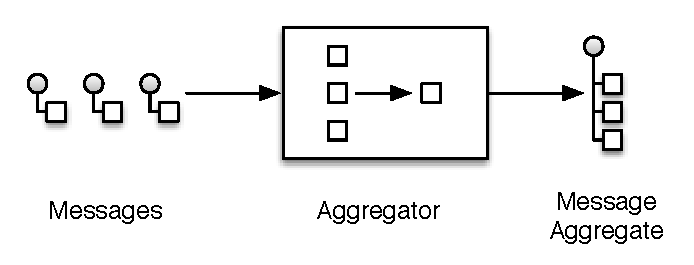
\includegraphics[width=0.7\textwidth]{ch02_aggregator}
	\caption{Aggregator \citep{Hohpe:2003fk}}
	\label{fig:ch02_aggregator}
\end{figure}

It is defined by the following properties:
\begin{itemize}
	\item \textbf{Correlation}\\
	Defines which messages should be correlated with each other.
	\item \textbf{Completeness Condition}\\
	Defines when a set of messages is ready to be written to the output channel.
	\item \textbf{Aggregation Algorithm}\\
	Defines how the received messages should be aggregated to a single message.
\end{itemize}

\cite{Hohpe:2003fk} describe the following most common strategies for completeness conditions:
\begin{itemize}
	\item \textbf{Wait for All}\\
	The aggregation is completed, when all messages are received. 
	\item \textbf{Timeout}\\
	The aggregation is completed when a defined timout occurs.
	\item \textbf{First Best}\\
	The \emph{Aggregator} waits until the first message is received.
	\item \textbf{Timeout with Override}\\
	The \emph{Aggregator} waits until a defined timeout occurs or until a message with a special content is received.
	\item \textbf{External Event}\\
	The aggregation is completed by an external event, for example the end of a business day.
\end{itemize}

Additionally, the authors describe the following strategies to aggregate messages into a single message \citep{Hohpe:2003fk}:
\begin{itemize}
	\item \textbf{Select the best answer}\\
	Only the ``best'' messages is passed to the output channel, all other messages are dismissed, for example the lowest bid for an item.
	\item \textbf{Condense data}\\
	The message data is aggregated into a single value, for example computing an average or a sum of a numerical value.
	\item \textbf{Collect data for later evaluation}\\
	Messages are simply combined into a single message. The decision how to aggregate can be done later by another component.
\end{itemize}

\subsubsection{Message Router}
The \emph{Message Router} reads messages from an input message channel and sends it to different output channels, depending on a set of conditions defined in the \emph{Message Router} (see Figure \ref{fig:ch02_message_router}).

\begin{figure}[htbp]
	\centering
	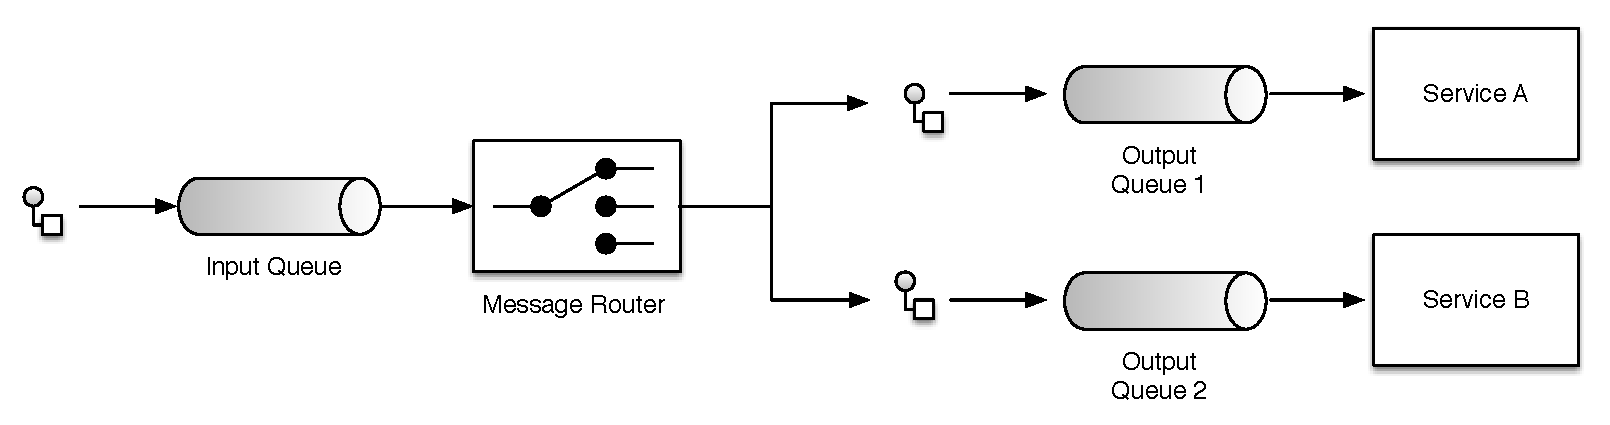
\includegraphics[width=\textwidth]{ch02_router}
	\caption{Message Router \citep{Hohpe:2003fk}}
	\label{fig:ch02_message_router}
\end{figure}

A \emph{Message Router} can implement different types of message routing:
\begin{itemize}
	\item \textbf{Content-based routing}\\
	The routing is based on the properties of a message, for example the message type or some business specific rules.
	\item \textbf{Context-based routing}\\
	The routing is based on conditions of the environment. This is used for example for load-balancing or failover strategies.
	\item \textbf{Dynamic routing}\\
	The routing is based on a dynamic rule base, which can be adapted at run-time.
\end{itemize}

\subsubsection{Content Filter}
A \emph{Content Filter} removes or simplifies unneeded data items from a message, only needed data items are left (see Figure \ref{fig:ch02_content_filter}).

\begin{figure}[htbp]
	\centering
	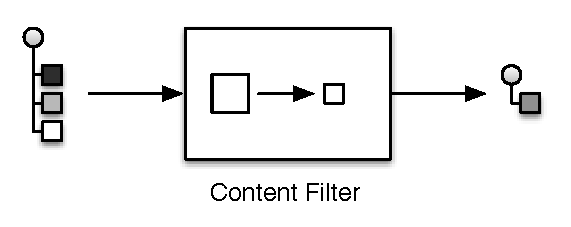
\includegraphics[width=0.6\textwidth]{ch02_content_filter}
	\caption{Content Filter \citep{Hohpe:2003fk}}
	\label{fig:ch02_content_filter}
\end{figure}

\subsubsection{Claim Check}

Since messaging adds an additional overhead to the processing of each message, for example by serializing and deserializing of data, it may be inefficient to send large volumes of data over a messaging system (cf. \cite{Hohpe:2003fk}). The \emph{Claim Check} pattern can used to mitigate this problem. It stores the payload of a message in a persistent data store and passes a unique identifier, the claim check, to the next components. Using this identifier, a component can retrieve the message payload from the data store and process the message (see Figure \ref{fig:ch02_claim_check}).

\begin{figure}[htbp]
	\centering
	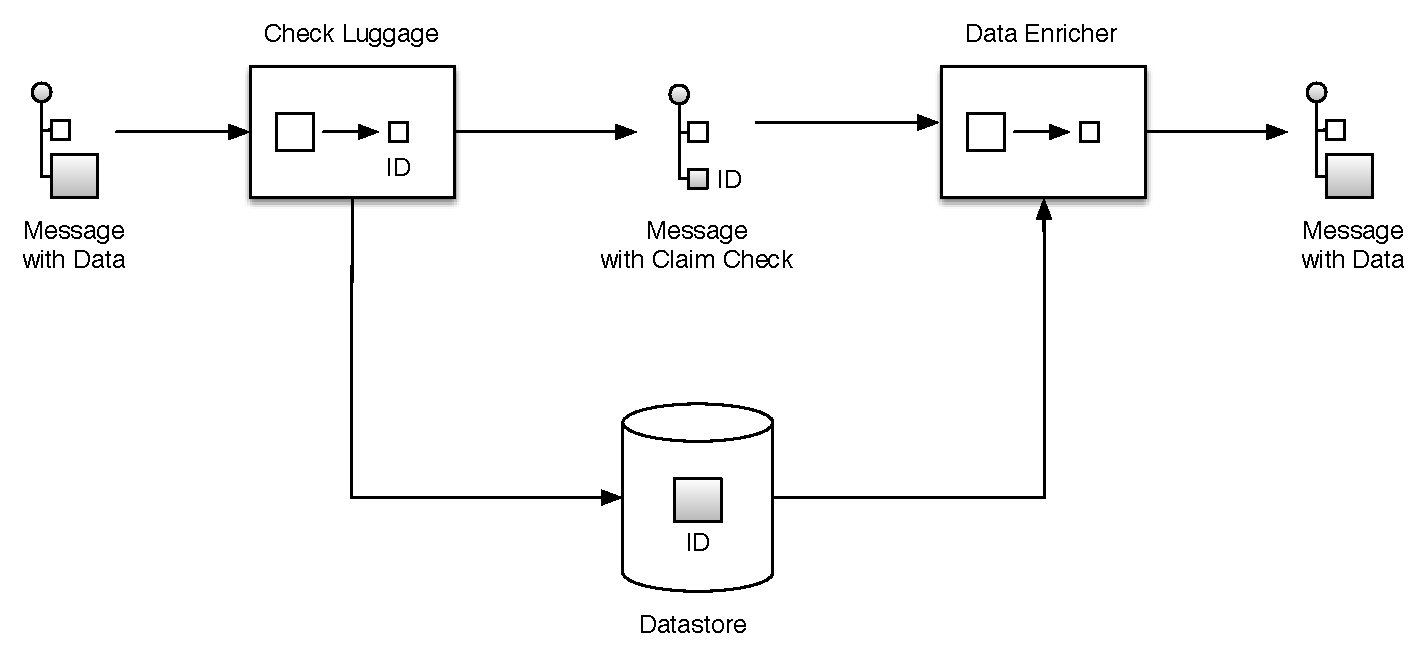
\includegraphics[width=\textwidth]{ch02_claim_check}
	\caption{Claim Check \citep{Hohpe:2003fk}}
	\label{fig:ch02_claim_check}
\end{figure}

\section{Performance Issues of Service-Oriented Middleware}
\label{sec:ch02_performance_issues}
This section describes the performance issues of an SOA middleware that inhibit their appropriateness for systems with high performance requirements.
\subsection{Distributed Architecture}
A system implemented according to the principles of SOA is a distributed system. Services are hosted on different locations belonging to different departments and even organizations. Hence, the performance drawbacks of a distributed system generally also apply to SOA. This includes the marshalling of the data that needs to be sent to the service provider by the service consumer, sending the data over the network and the unmarshalling of data by the service provider.
\subsection{Integration of Heterogeneous Technologies}
A main goal of introducing an SOA is to integrate applications implemented with heterogeneous technologies. This is achieved by using specific middleware and intermediate protocols for the communication. These protocols are typically based on XML, like SOAP \citep{soap:2007}. XML, as a very verbose language, adds a lot of meta-data to the actual payload of a message. The resulting request is about 10 to 20 times larger than the equivalent binary representation \citep{OBrien:2007fk}, which leads to a significant higher transmission time of the message. Processing these messages is also time-consuming, as they need to get parsed by a XML parser before the actual processing can occur.

The usage of a middleware like an Enterprise Service Bus (ESB) adds further performance costs. An ESB usually processes the messages during transferring. Among other things, this includes the mapping between different protocols used by service providers and service consumers, checking the correctness of the request format, adding message-level security and routing the request to the appropriate service provider (See, for example, \citet{Josuttis:2007fk} or \citet{Krafzig:2005zc}).
\subsection{Loose Coupling}
Another aspect of SOA that has an impact on performance is the utilisation of loose coupling. The aim of loose coupling is to increase the flexibility and maintainability of the application landscape by reducing the dependency of its components on each other. This denotes that service consumers shouldn't make any assumptions about the implementation of the services they use and vice versa. Services become interchangeable as long they implement the interface the client expects.

\citet{Engels:2008nr} consider two components A and B loosely coupled when the following constraints are satisfied:
\begin{itemize}
	\item \textbf{Knowlegde}\\
	Component A knows only as much as it is needed to use the operations offered by component B in a proper way. This includes the syntax and semantic of the interfaces and the structure of the transferred data.
	\item \textbf{Dependence on availability}\\
	Component A provides the implemented service even when component B is not available or the connection to component B is not available.
	\item \textbf{Trust}\\
	Component B does not rely on component A to comply with pre-conditions. Component A does not rely on component B to comply with post-conditions.
\end{itemize}

Coupling between services occurs on different levels. \citet{Krafzig:2005zc} describe the different levels of coupling that are leveraged in an \ac{SOA} (see Table \ref{table:ch02_coupling}).

\begin{table}[htpb]
	\centering
	\begin{tabularx}{\textwidth}{@{} X X X @{}}
		\caption{Levels of coupling}\label{table:ch02_coupling}\\
		\toprule
		\bfseries Level & \bfseries Tight Coupling & \bfseries Loose Coupling\\
		\midrule
		\bfseries Physical coupling & Direct physical link required & Physical intermediary\\
		\midrule
		\bfseries Communication style & Synchronous & Asynchronous\\
		\midrule
		\bfseries Type system & Strong type system & Weak type system\\
		\midrule
		\bfseries Interaction pattern & OO-style navigation of complex object trees & Data-centric, self-contained messages\\
		\midrule
		\bfseries Control of process logic & Central control of processing logic & Distributed logical components\\
		\midrule
		\bfseries Service discovery and binding & Statically bound services & Dynamically bound services\\
		\midrule
		\bfseries Platform dependencies & Strong OS and programming language dependencies & OS and programming languages independent\\
		\bottomrule
	\end{tabularx}
\end{table}

The gains in flexibility and maintainability of loose coupling are amongst others opposed by performance costs.

Service consumers and service providers are not bound to each other statically. Thus, the service consumer needs to determine the correct end point of the service provider during runtime. This can be done by looking up the correct service provider in a service repository either by the service consumer itself before making the call or by routing the message inside the ESB.  

Apart from very few basic data types, Service consumers and service providers do not share the same data model. It is therefore necessary to map data between the data model used by the service consumer and the data model used by the service provider.
\section{Current Approaches for Improving the Performance of an SOA Middleware}
This section describes current approaches to the performance issues introduced in the previous section.
\subsection{Hardware}
The obvious solution to improve the processing time of a service is the utilization of faster hardware and more bandwidth. SOA performance issues are often neglected by suggesting that faster hardware or more bandwidth will solve this problem. However, it is often not feasible to add faster or more hardware due to high cost pressure.
\subsection{Compression}
The usage of XML as an intermediate protocol for service calls has a negative impact on their transmission times over the network. The transmission time of service calls and responses can be decreased by compression. Simply compressing service calls and responses with gzip can do this. The World Wide Web Consortium (W3C) proposes a binary presentation of XML documents called binary XML \citep{EXI:2007} to achieve a more efficient transportation of XML over networks.

It must be pointed out that the utilisation of compression adds the additional costs of compressing and decompressing to the overall processing time of the service call.
\subsection{Service Granularity}
To reduce the communication overhead or the processing time of a service, the service granularity should be reconsidered.

\cite{Haesen:2008ve} distinguishes between two types of data granularity:
\begin{itemize}
	\item \textbf{Input data granularity}\\
	Data that is sent to a component
	\item \textbf{Output data granularity}\\
	Data that is returned by a component
\end{itemize}
The authors state that a coarse-grained data granularity reduces the communication overhead, since the number of network transfers is decreased.
``Especially in the case of Web services, this overhead is high since asynchronous messaging requires multiple queuing operations and numerous XML transformations''.

Coarse-grained services reduce the communication overhead by achieving more with a single service call and should be the favoured service design principle \citep{Hess:2006rs}. However, the processing time of a coarse-grained service can pose a problem to a service consumer that only needs a fracture of the data provided by the service. To reduce the processing time it could be considered in this case to add a finer grained service that provides only the needed data \citep{Josuttis:2007fk}. 

It should be noted that merging multiple services to form a more coarse-grained service or splitting a coarse-grained service into multiple services to solve performance problems specific to a single service consumer reduces the reusability of the services for other service consumers \citep{Josuttis:2007fk}.
\subsection{Degree of Loose Coupling}
The improvements in flexibility and maintainability gained by loose coupling are opposed by drawbacks on performance. Thus, it is crucial to find the appropriate degree of loose coupling. 

\citet{Hess:2006rs} introduce the concept of distance to determine an appropriate degree of coupling between components. The distance of components is comprised of the functional and technical distance. Components are functional distant if they share few functional similarities. Components are technical distant if they are of a different category. Categories classify different types of components like inventory components, process components, function components and interaction components.

Distant components trust each other in regard to the compliance of services levels to a lesser extent than near components do. The same applies to their common knowledge. Distant components share a lesser extent of knowledge of each other. Therefore, \citet{Hess:2006rs} argue that distant components should be coupled more loosely than close components.

The degree of loose coupling between components that have been identified to be performance bottlenecks should be reconsidered to find the appropriate trade-off between flexibility and performance. It can be acceptable in that case to decrease the flexibility in favour of a better performance. 

\subsection{Scaling}
Scalability describes the ``ability of a system to accommodate an increasing number of elements or objects, to process growing volumes of work gracefully, and/or to be susceptible to enlargement'' \citep{Bondi:2000jr}.

\cite{weinstock2006system} define scalability as:
\begin{enumerate}
	\item The ability to handle increased workload (without adding resources to a system).
	\item The ability to handle increased workload by repeatedly applying a cost-effective strategy for extending a system's capacity.
\end{enumerate}

\begin{itemize}
	\item \textbf{Horizontal scaling}\\
	Horizontal scaling involves adding more nodes to system, for example adding more servers to a distributed system and using a load-balancer to distribute the work between them.
	\item \textbf{Vertical scaling}\\
	Vertical scaling involves adding more resources to single node, such as additional \acp{CPU} or memory.
\end{itemize}

When a system is faced with infrequent load spikes, static scaling can lead to an overprovisioning of resources. The system is optimized to handle the load spikes, but is idle during the rest of the time.

\subsection{Dynamic Scaling}
A solution to prevent overprovisioning and to handle infrequent load spikes is to automatically instantiate additional server instances, as provided by current \ac{PaaS} offerings such as Amazon EC2 \citep{ec2_autoscaling} or Google App Engine \citep{google_cloud_autoscaling}. This is also called elasticity in the context of cloud computing (cf. \cite{Herbst:2013ug}).

While scaling is a common approach to improve the performance of a system, it also leads to additional operational and possible license costs. The solution presented in this thesis can be combined with these auto-scaling approaches to further increase the performance of the system.

\section{Summary}
Systems for bulk data processing are traditionally implemented using batch processing, for example billing systems for telecommunication providers. The performance requirements for such systems are high. They have to process millions of records in a fixed timeframe to comply with service level agreements.

Message-oriented middleware facilitates the integration of applications using asynchronous messages. Message-based systems are able to provide near-time processing of data due to their lower latency compared with batch processing systems. The advantage of a lower latency comes with a performance cost in regard to a lower throughput because of the additional overhead for each processed message. Every message needs amongst others to be serialised and deserialised, mapped between different protocols and routed to the appropriate receiving system. In the context of an \ac{SOA}, an Enterprise Service Bus is a common messaging middleware combining messaging, web services, data transformation and intelligent routing.

Common approaches to improve the performance of message-based systems try to reduce the transmission time by compressing messages, to adjust the service granularity to form more coarse-grained services or to adjust the degree of loose coupling to reduce the communication overhead. Scaling is a common approach to optimize the performance of of data processing system. Dynamic scaling is another solution to handle infrequent load spikes.

While these approaches generally improve the performance of mes\-sage-based systems, they are still not able provide the same throughput as that can be achieved with a batch processing system. Additionally, the current approaches are static and thus need to be considered at the design-time of the system. 

Systems are currently either optimized for bulk data processing or low latency. Alternatively, they use different components for batch and real-time processing. The proposed approached in this thesis, a middleware that is able to adapt its processing style fluently based on the current load of the system is a new approach which has not be considered so far by the state of art to the best of the author's knowlegde.
\cleardoublepage%!TEX root = ../thesis.tex
%******************************************************************************
\chapter{Related Work}\label{ch:relatedwork}
%******************************************************************************

This chapter gives an overview of work related to this PhD project (see figure \ref{fig:related_work_map}). It starts with work that addresses the performance of Service-Oriented systems in general. Further work in the area of SOA performance can be classified into the categories performance modeling, performance measuring and performance optimisation.

The proposed middleware for high-performance near-time processing of bulk data adjusts the data granularity itself at runtime. Work on middleware discusses different approaches for self-adjustment and self-awareness of middleware, which can be classified as adaptive or reflective middleware, discussed in the next section.

In order to dynamically adjust the data granularity at runtime, the proposed middleware needs to constantly measure the throughput and latency of the system. Work on SLA-monitoring proposes different approaches to monitor the compliance of business processes to Service Level Agreements.

Finally, the chapter concludes with a summary which relates the discussed approaches to the approach proposed in this PhD project.
\begin{figure}[htbp]
	\centering
	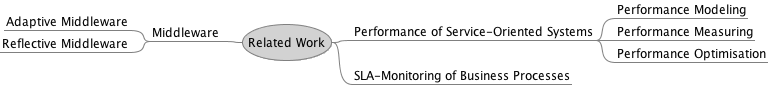
\includegraphics[width=\textwidth]{img/related_work_map.png}
	\caption{Related Work}
	\label{fig:related_work_map}
\end{figure}
\section{Performance of Service-Oriented Systems}
\citet{OBrien:2007fk} argue that the introduction of an SOA generally has a negative impact on the performance of the system. They identify the following key aspects responsible for the performance degradation:
\begin{itemize}
	\item \textbf{Network communication}\\
	Service provider and service consumer need to communicate over a network, which usually does not offer a deterministic latency.
	\item \textbf{Lookup of services in a directory}\\
	The lookup of a service provider in a directory increases the total transaction time of a service request.
	\item \textbf{Interoperability of services on different plattforms}\\
	The interoperability of services on different platforms is realized by a middleware which handles the whole communication. The needed marshalling and unmarshalling of data adds a performance overhead to the communication.
	\item \textbf{Usage of standard messaging formats}\\
	The usage of a standard message format, like XML, increases the processing time of a service due to parsing, validation and transformation of messages. An XML message can be 10 to 20 times larger than the binary representation which increases the the transport time of the message over the network.
\end{itemize}
In another paper, \citet{OBrien:2008uq} state that the performance issues of an SOA are caused by:
\begin{itemize}
	\item Overhead of XML
	\item Implementation of composite services
	\item Service orchestration
	\item Service invocation
	\item Resources, e.g. threads, CPUs
	\item Resource models, e.g. virtualization
\end{itemize}
The authors suggest that it is vital to consider performance aspects early in the development lifecycle, which can be supported by using an SOA performance model.

\citet{Woodall:2007kx} describe in their paper the challenges they encountered when analysing a performance problem of a concrete Service-Oriented System:
\begin{itemize}
	\item Physical distribution of services
	\item Continual use of services by local users or developers during the performance investigation
	\item Heterogeneity of the underlying service software plattform
\end{itemize}
\section{Performance Modeling}
Performance modeling allows to predict the performance of a system in an early stage of development. It facilitates for example capacity and resource planning before the system is already available or helps to evaluate design alternatives in regard of their performance impact.

\citet{Brebner:2008uq} developed a tool for performance modeling of Service-Oriented Architectures. It is comprised of SOA models, a simulation engine and a graphical user interface. The SOA models are generated from architectural artifacts such as UML sequence or deployment diagrams and automatically transformed into runtime models for execution.

An approach to predict the performance of J2EE applications using messaging services using queueing network models has been presented by \citet{Liu:2007vn}. As opposed to prior approaches, their solution models the underlying component infrastructure that implements the messaging service which allows an accurate prediction with an error within 15\% when compared to the real performance of the implemented system.

In another work, \citet{Liu:2007vn} developed a performance model of an service-oriented application based on an Enterprise Service Bus using a queuing network. Their modeling approach includes the following steps:
\begin{itemize}
	\item Mapping of application components of the design level to analytical model elements
	\item Characterisation of workload patterns for the application components used as input for performance model
	\item Calibrating the performance model
	\item Validating the performance model
\end{itemize}

\citet{DAmbrogio:2007ly} describe ``a model-driven approach for integrating performance prediction into service composition processes carried out by use of BPEL (Business Process Execution Language for Web Services).'' Using their approach, a BPEL process is described using an UML model. The model is automatically annotated with performance data and transformed into a Layered Queueing Network which is used to predict the performance of the BPEL process. For the automatic annotation of the model, a performance-oriented extension to WSDL is utilised called P-WSDL \citep{D-Ambrogio:2005ve}.
\section{Performance Measuring}
Performance measuring is applied to evaluate if an implemented system meets its performance requirements and to spot possible performance problems.

\citet{Her:2007qf} propose the following set of metrics for measuring the performance of a service-oriented system:
\begin{itemize}
	\item \textbf{Service response time}\\
	Elapsed time between the end of request to service and the beginning of the response of the service. This metric is further split in 20 sub-metrics such as message processing time, service composition time and service discovery time.
	\item \textbf{Think time}\\
	Elapsed time between the end of a response generated by a service and the beginning of a response of an end user.
	\item \textbf{Service tournaround time}\\
	Time needed to get the result from a group of related activities within a transaction.
	\item \textbf{Throughput}\\
	Number of requests served at a given period of time. The authors distinguish between the throughput of a service and the throughput of a business process.
\end{itemize}

In their work, \citeauthor{Henjes:2006nx} investigated the throughput performance of the JMS server FioranaMQ, SunMQ and WebsphereMQ. The authors came to the following conclusion (\citet{Henjes:2006nx} and \citet{Menth:2006qe}):
\begin{itemize}
	\item Message persistence reduces the throughput significantly.
	\item Message replication increases the overall throughput of the server.
	\item Throughput is limited either by the processing logic for small messages or by the transmission capacity for large messages.
	\item Filtering reduces the throughput significantly.
\end{itemize}

\citet{Chen:2004cr} propose that the following performance metrics should be used to evaluate a JMS server:
\begin{itemize}
	\item Maximum sustainable throughput
	\item Latency
	\item Elapsed time taken to send batches messages
	\item Persistent message loss after recovery
\end{itemize}
The authors state that ``although messaging latency is easy to understand, it is difficult to measure precisely in a distributed environment without synchronised high- precision clocks.'' They discovered that latencies increase with increasing message sizes.

SPECjms2007 is a standard benchmark for the evaluation of Message-Oriented Middleware platforms using JMS \citep{Sachs:2009rr}. It provides a flexible performance analysis framework for tailoring the workload to specific user requirements. According to \citet{sachs2007designing}, the workload of the SPECjms2007 benchmark has to meet the following requirements:
\begin{itemize}
	\item \textbf{Representativeness}\\
	The workload should reflect how the messaging platform is used in typical user scenarios.
	\item \textbf{Comprehensiveness}\\
	The workload should incorporate all platform features typically used in JMS application including publish/subscript and point-to-point messaging.
	\item \textbf{Focus}\\
	The workload should focus on measuring the performance of the messaging middleware and should minimize the impact of other components and services.
	\item \textbf{Configurability}\\
	It should be possible to configure the workload to meet the requirements of the user.
	\item \textbf{Scalability}\\
	It should be possible to scale the workload by the number of destinations with a fixed traffic per destination or by increasing the traffic with a fixed set of destinations.
\end{itemize}
\section{Performance Optimisation}
Most of the work that aims to optimise the performance of service-oriented systems is done in the area of Web Services since it is a common technology to implement a SOA.

In particular, various approaches have been proposed to optimise the performance of SOAP, the standard protocol for Web Service communication. This includes approaches for optimising the processing of SOAP messages (see for example \citet{Abu-Ghazaleh:2005bs}, \citet{Suzumura:2005fv} and \citet{Ng:2006kl}), compression of SOAP messages (see for example \citet{Estrella:2008dz} and \citet{Ng:2005qa}) and caching (see for example \citet{andresen2004lye} and \citet{Devaram:2003fu}).

\citet{Wichaiwong:2007oq} propose an approach to transfer bulk data between web services per FTP. The SOAP messages transferred between the web services would only contain the necessary details how to download the corresponding data from an FTP server since this protocol is optimized for transferring huge files. This approach solves the technical aspect of efficiently transferring the input and output data but does not pose any solutions how to implement loose coupling and how to integrate heterogeneous technologies, the fundamental means of an SOA to improve the flexibility of an application landscape.

Data-Grey-Box Web Services are an approach to transfer bulk data between Web Services \citep{Habich:2007ij}. Instead of transferring the data wrapped in SOAP messages, it is transferred using an external data layer. For example when using database systems as data layer, this facilitates the use of special data transfer methods such ETL (Extract, Transform, Load) to transport the data between the database of the service requestor and the database of the Web service. The data transfer is transparent for both service participants in this case. The approach includes an extension of the Web service interface with properties describing the data aspects. Compared to the SOAP approach, the authors measured a speedup of up to 16 using their proposed approach. To allow the composition and execution of Data-Grey-Box Web services,  \citet{Habich:kl} developed BPEL data transitions to explicitly specify data flows in BPEL processes.
\section{Self-Adaptive Middleware}
Self-Adaptive Software is a ``a closed-loop system with a feedback loop aiming to adjust itself to changes during its operation'' \citep{Salehie:2009pi}. These changes can originate from internal causes of the system (the system's self) or from the context of the system.

\citet{Laddaga:2008ff} provides a definition for self-adaptive software: ``Self-adaptive software evaluates its own behavior and changes behavior when the evaluation indicates that it is not accomplishing what the software is intended to do, or when better functionality or performance is possible.'' 

Another definition is given by \citet{Oreizy:1999lh}: ``Self-adaptive software modifies its own behavior in response to changes in its operating environment. By operating environment, we mean anything observable by the software system, such as end-user input, external hardware devices and sensors, or program instrumentation.''

\cite{Salehie:2009pi} describe the following properties (also called self-* properties) of a self-adaptive system:
\begin{itemize}
	\item \textbf{Self-configuring}\\
	The system is able to reconfigure itself in response to changes.
	\item \textbf{Self-healing}\\
	The system is able to discover, diagnose and react on failures.
	\item \textbf{Self-optimizing}\\
	The system is able to manage performance and resource allocation to meet different performance requirements.
	\item \textbf{Self-protecting}\\
	The system is able to detect security breaches and to recover from them.
\end{itemize}

More general self-* properties are described as:
\begin{itemize}
	\item \textbf{Self-Awareness}\\
	The system is aware of its self states and behaviours.
	\item \textbf{Context-Awareness}\\
	The system is aware of its context.
\end{itemize}

\citet{Duran-Limon:2004mi} argue that ``the moste adequate level and natural locus for applying adaption is at the middleware level''. Adaption at the operating system level is platform-dependent and changes at this level affect every application running on the same node. On the other hand, adaption at application level assigns the responsibility to the developer and is also not reusable.

\citet{Lee:2009vn} propose an adaptive, general-purpose runtime infrastructure for effective resource management of the infrastructure. Their approach is comprised of three components:
\begin{enumerate}
	\item dynamic performance prediction
	\item adaptive intra-site performance management
	\item adaptive inter-site resource management
\end{enumerate}

The runtime infrastructure is able to choose from a set of performance predictions for a given service and to dynamically choose the most appropriate prediction over time by using the prediction history of the service.

AutoGlobe \citep{Gmach:2008vo} provides a platform for adaptive resource management comprised of 
\begin{enumerate}
	\item Static resource management
	\item Dynamic resource management
	\item Adaptive control of Service Level Agreements (SLA)
\end{enumerate}
Static resource management optimises the allocation of services to computing resources and is based on on automatically detected service utilisation patterns. Dynamic resource management uses a fuzzy controller to handle exceptional situations at runtime. The Adaptive control of Service Level Agreements schedules service requests depending on their SLA agreement.

The coBRA framework proposed by \citet{Irmert:2008nx} is an approach to replace service implementations at runtime as a foundation for self-adaptive applications. The framework facilitates the replacement of software components to switch the implementation of a service with the interface of the service staying the same.

DREAM (Dynamic Reflective Asynchronous Middleware) \citep{Leclercq:2004ly} is a component-based framework for the construction of reflective Message-Oriented Middleware. Reflective middleware ``refers to the use of a causally connected self-presentation to support the inspection and adaption of the middleware system'' \citep{Kon:2002fu}. DREAM is based on FRACTAL, a generic component framework and supports various asynchronous communication paradigms such as message passing, event-reaction and publish/subscribe. DREAM facilitates the construction and configuration of Message-Oriented Middleware from a library of components such as message queues, filters, routers and aggregators, which can be assembled either at deploy-time or runtime.
\section{SLA-Monitoring of Business Processes}
The SECMOL framework (Service Centric Monitoring Language), developed by \citet{Guinea:2009fk}, allows to monitor the quality of service constraints of BPEL processes. It is comprised of three components. Data Collectors for capturing data, Data Analyzers for analysing the captured data and the Monitoring Manager for coordinating the monitoring process. SECMOL also defines a XML-based monitoring specification, which consists of monitoring policies that specify how the monitoring should be done and monitoring rules that express the quality of service properties the system needs to satisfy.

\citet{Duc:2009kx} argue that a monitoring middleware component should fulfill the following requirements:
\begin{itemize}
	\item \textbf{Coherency of data}\\
	All data used in one decision must reflect the same state of the system.
	\item \textbf{Flexibility in data access}\\
	Every monitored service provider should be able to respond using its own measurement units. This should be transparent for the client using the monitoring data.
	\item \textbf{Performance in data access}\\
	The monitoring should have the slightest possible impact on the performance of the business process.
	\item \textbf{Network usage optimisation}\\
	The transmission of monitoring data should have the slightest possible impact on the network performance.
\end{itemize}
The authors propose M4ABP (Monitoring for Adaptive Business Process), a distributed monitoring and data delivery middleware subsystem, which implements these requirements.

SALMon \citep{Ameller:2008zr} is a system for monitoring the services of an SOA for Service Level Agreement violations. It is itself implemented as an service-oriented system and consists of the following services:
\begin{itemize}
	\item \textbf{Monitor}\\
	The Monitor service collects the monitoring data from components called Measure Instruments that are instantiated in each monitored service. 
	\item \textbf{Analyzer}\\
	The Analyzer service manages the Monitor service and checks for Service Level Agreement violations of the monitored services.
	\item \textbf{Decision Maker}\\
	The Decision Maker service is able to select an action to solve the SLA violation. The appropriate action for a specific SLA violation is stored in a repository.
\end{itemize}
The attributes measured by SALMon are taken from an ISO/IEC 9126-1-based quality model.

\citet{Textor:2009vn} propose an approach to map implementation level monitoring data to business level activities. Non-functional constraints are specified on a workflow model in the modelling phase. Additionally, an instrumentation model is used to specify the instrumentation points of the application. At runtime, the monitoring data of the system is mapped to the workflow model. 
The monitoring data is received by a component called ConstraintMonitor, which evaluates and validates the constraints specified in the workflow model.

\citet{Wetzstein:2009uq} present a framework to monitor and analyse the factors that influence the performance of WS-BPEL processes. The authors distinguish between PPM (Process Performance Metrics) and QoS (Quality of Service) metrics, which influence the Key Performance Indicators (KPI) of business processes. PPMs are based on process runtime events, that are published by the WS-BPEL runtime engine, for example the ``number of orders which can be served as inhouse stock''. QoS metrics are technical parameters of the underlying services that implement the business process, for example the response time and availability of a service. KPIs are based on business goals, for example ``order fulfillment lead time < 3''. The proposed framework monitors KPIs, PPMs and QoS metrics at runtime, which are modeled in a Process Metrics Definition Model (PMDM). These collected metrics can then be used to perform a dependency analysis of the influential factors of a KPI using machine learning techniques to construct dependency trees.

iBOM \citep{Castellanos:2005fk} is a platform to analyse, manage and optimise business operations based on business goals. Optimisations are performed by using simulation techniques. iBom simulates different configurations of a business process to identify the configuration that best meets the business goals. First, the user needs to define the optimisation metric and constraints on this metric and on the resources. The configuration candidates are then either computed by iBOM using different resource allocations of the given configuration within the defined constraints or are provided by the user in the form of a process model. 

\section{Summary}
Most of the work done in the field of performance of service-oriented systems involves performance aspects of Web Services including the SOAP standard. This includes performance modeling, performance measuring and performance optimisation. 

Approaches to optimise the transfer of bulk data of Web services, as proposed by \citet{Wichaiwong:2007oq} and  \citet{Habich:2007ij} deliver an overall better performance than using SOAP. However, like a traditional batch-processing system using file- or database-based integration, they are not able to reduce the latency and thus cannot deliver near-time processing of bulk data.

Current self-adapting middleware platforms, like the AutoGlobe platform \citep{Gmach:2008vo}, are focused on adaptive resource management to dynamically allocate services to computing nodes or to replace service implementations at runtime, as proposed by the coBRA framework \citep{Irmert:2008nx}.

Work on SLA-monitoring of business processes proposes different approaches to monitor the compliance of a business process to Service Level Agreements, which include the end-to-end latency and throughput of the business process. However, they do not propose any solutions for improving the end-to-end latency in order to provide near-time processing of bulk data.

The research project presented in this report proposes an adaptive middleware to reduce the latency of a system for bulk data processing by dynamically adjusting the data granularity at runtime based on the current throughput and the minimum acceptable throughput of the system. To the best of our knowledge, this is a novel approach which has not yet been discussed in current literature.
\cleardoublepage
\part{Contributions}
\cleardoublepage%!TEX root = ../thesis.tex
%******************************************************************************
\chapter{Performance Evaluation of Batch and Message-based Systems}\label{ch:performance_evaluation}
%******************************************************************************

\section{Introduction}\label{sec:ch4_introduction}

Traditionally, business information systems for bulk data processing are implemented as batch processing systems. Batch processing delivers high throughput but cannot provide near-time processing of data, that is the end-to-end latency of such a system is high. 

A lower end-to-end latency can be achieved by using message-based processing, for example by utilising a message-oriented middleware for the integration of the services that form the business information system. While this approach is able to deliver near-time processing, it is hardly capable for bulk data processing due to the additional communication over- head for each processed message. Therefore, message-based processing is ususally not considered for building a system for bulk data processing requiring high throughput.

This chapter compares the performance of a batch and message-based system. The main objectives of this comparison are:

\begin{itemize}
  \item What is the impact of different processing styles, that is batch and message-based processing, on throughput and latency?
  \item What is the impact of data granularity on latency and throughput when using a message-based processing style?  
\end{itemize}

To find solutions for these questions, the following approach has been taken:

\begin{itemize}
	\item Two prototypes of a billing system for each processing type (see Section \ref{sec:ch4_prototype}) have been built. 
	\item A performance evaluation has been conducted to compare the prototypes with each other with the focus on throughput and latency (see Section \ref{sec:ch4_evaluation}).
	\item To evaluate the impact of different aggregatation sizes on throughput and latency, the messaging prototype has been extended with an aggregator. A performance test has been conducted with different static aggregation sizes (see Section \ref{sec:ch4_impact_granularity}).
\end{itemize}

This chapter is organised as follows. Section \ref{sec:ch4_prototype} introduces the batch and message-based prototype systems that have been implemented. To compare the performance characterics of the two processing types, batch processing and message-based processing, a performance evaluation has been conducted, which is presented in Section \ref{sec:ch4_evaluation}. Section \ref{sec:ch4_impact_granularity} shows the impact of data granularity on throughput and latency of the messaging prototype. Section \ref{sec:ch4_related_work} gives an overview of other work related to the contents of this chapter. Finally, this chapter concludes with a summary in Section \ref{sec:ch4_summary} 

\section{A real world example  application}\label{sec:ch4_prototype}
This section introduces the two prototypes of a billing system that have been built to evaluate the performance of batch and message-based processing.

A billing system is a distributed system consisting of several sub components that process the different billing sub processes like mediation, rating, billing and presentment (see Figure \ref{fig:ch4_billing_process}).



\begin{figure}[htbp]
	\centering
	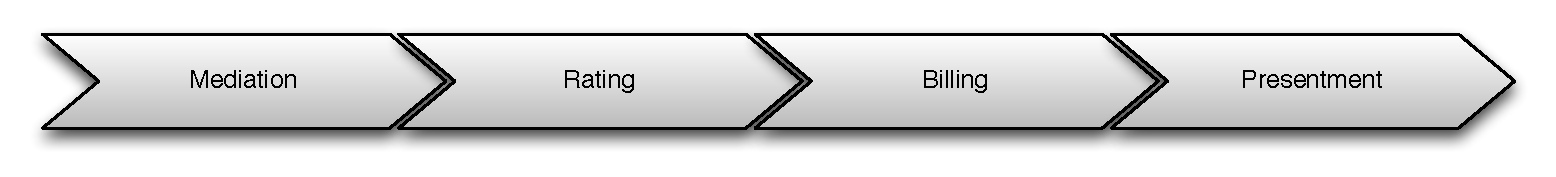
\includegraphics[width=\columnwidth]{billing_process}
	\caption{Billing process}
	\label{fig:ch4_billing_process}
\end{figure}

The mediation components receive usage events from delivery systems, like switches and transform them into a format the billing system is able to process. For example, transforming the event records to the internal record format of the rating and billing engine or adding internal keys that are later needed in the process. The rating engine assigns the events to the specific customer account, called guiding, and determines the price of the event, depending on the applicable tariff. It also splits events if more than one tariff is applicable or the customer qualifies for a discount. The billing engine calculates the total amount of the bill by adding the rated events, recurring and one-time charges and discounts. The output is processed by the presentment components, which format the bill, print it, or present it to the customer in self-service systems, for example on a website.

In order to compare batch and message-based types of processing, two different prototypes of a billing application have been developed. Each prototype implements the mediation and rating steps of the billing process. Figure \ref{fig:ch4_prototype_components} shows the components of the billing prototype: 
\begin{itemize}
	\item \textbf{Event Generator}\\
	The \emph{Event Generator} generates the calling events, i.e. the \ac{CDR} that are processed by the billing application.
	\item \textbf{Mediation}\\
	The \emph{Mediation} component checks wether the calltime of the calldetail record exceeds the minimal billable length or if it belongs to a flatrate account and sets the corresponding flags of the record. The output of the \emph{Mediation} component are \ac{NCDR} that are further processed by the \emph{Rating} component.
	\item \textbf{Rating}\\
	The \emph{Rating} component processes the output from the \emph{Mediation} component. It assigns the calldetail record to a customer account and determines the price of the call event by looking up the correspondant product and tariff in the \emph{Master Data DB}. The output of the \emph{Rating} component (costed events) is afterwards written to the \emph{Costed Events DB}.
	\item \textbf{Master Data DB}\\
	The \emph{Master Data DB} contains products, tariffs and accounts used by the \emph{Event Generator} and the \emph{Rating} component.
	\item \textbf{Costed Events DB}\\
	The \emph{Costed Events DB} contains the result of the \emph{Rating} component, i.e. the costed events.
\end{itemize}

\begin{figure}[htbp]
	\centering
	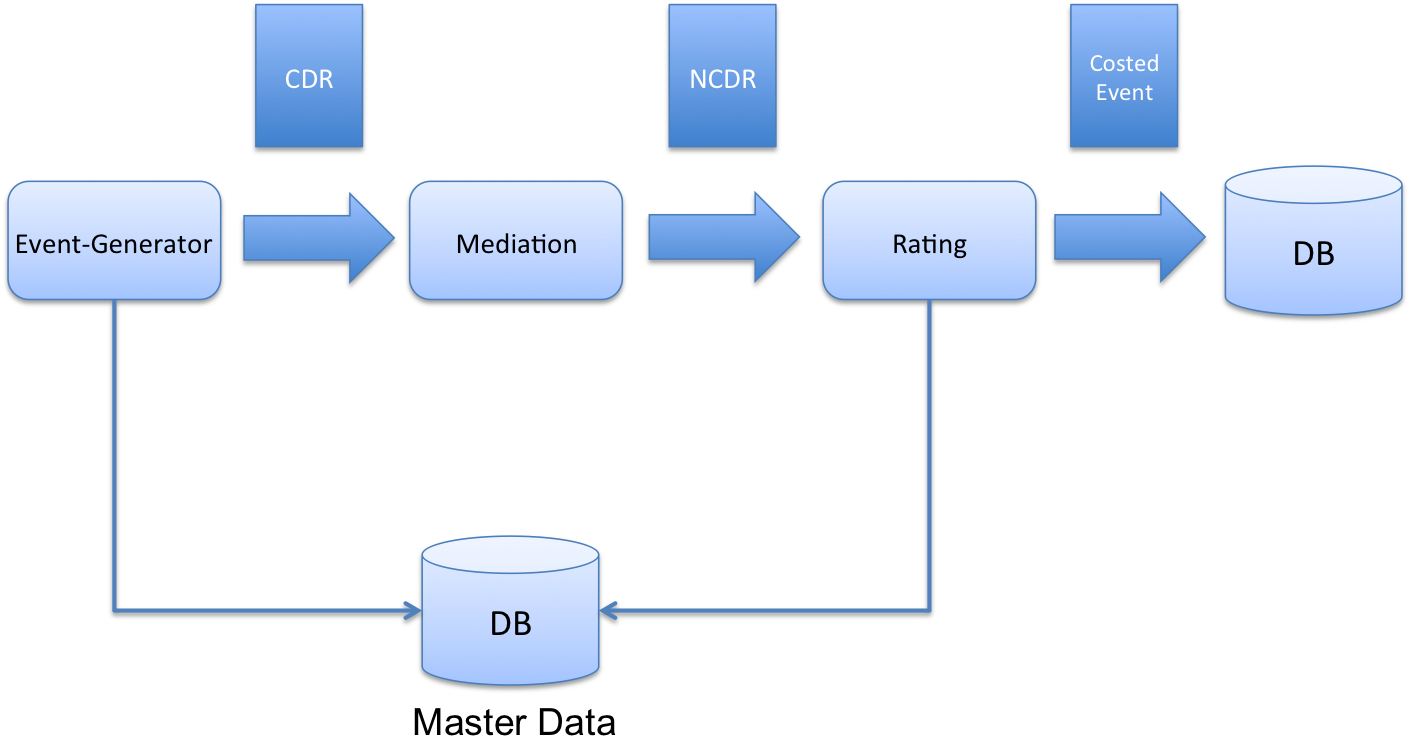
\includegraphics[width=\columnwidth]{prototype_components}
	\caption{Components of the billing application prototype}
	\label{fig:ch4_prototype_components}
\end{figure}

The prototypes are implemented with Java 1.6 using \ac{JPA} for the data-access layer and a MySQL database. See Table \ref{table:ch4_frameworks} for complete list of technologies and frameworks used for the implementation of the prototypes.

\begin{table}
	%\renewcommand{\arraystretch}{1.3}
	\centering
	\begin{tabularx}{\textwidth}{@{} l X @{}}
		\caption{Technologies and frameworks used for the implementation of the prototypes} \label{table:ch4_frameworks}\\
		\toprule
		\bfseries Language & Java 1.6\\
		\midrule
		\bfseries Dependancy Injection & Spring\\
		\midrule
		\bfseries Persistence API & OpenJPA (JPA 2.0)\\
		\midrule
		\bfseries Database & MySQL\\
		\midrule
		\bfseries Logging & Logback\\
		\midrule
		\bfseries Test & JUnit\\
		\midrule
		\bfseries Batch Framework & Spring Batch\\
		\midrule
		\bfseries Messaging Middleware & Apache Camel\\
		\midrule
		\bfseries Other Frameworks & Joda-Time, Apache Commons\\
		\bottomrule
	\end{tabularx}
\end{table}

\subsection{Common Architecture} % (fold)
\label{sub:ch4_common_architecture}

The objective of this performance evaluation is to compare the different processing styles, batch and single-event processing, with each other.
It needs to be ensured that the comparison only includes the different processing styles. Therefore, the prototypes should only differ in their processing style, all other aspects should be the same, for example the business functionality, data access and datamodel.

To ensure the comparability between the prototypes, a common architecture used by both prototypes has been designed and implemented.

It consists of the following components (see Figure \ref{fig:ch4_technical_integration}):

\begin{itemize}
	\item \textbf{Integration Layer}\\
	Implements the integration style, i.e. file-based integration and message-based integration.
	\item \textbf{Business Service}\\
	Implements the business functionality, i.e. mediation and rating.
	\item \textbf{Data Access Layer}\\Implements the data access.
\end{itemize}

\begin{figure}[htbp]
	\centering
	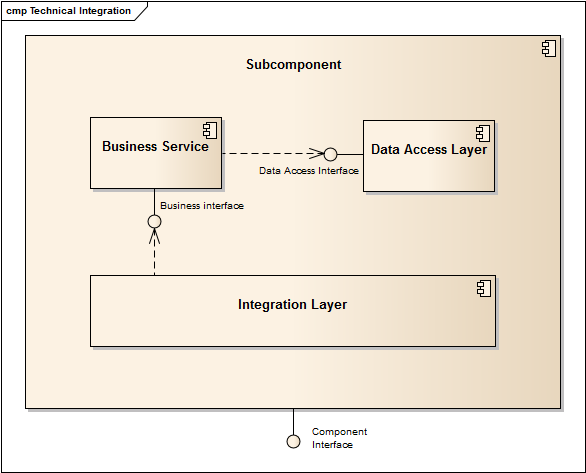
\includegraphics[width=0.7\textwidth]{technical_integration}
	\caption{The prototypes share the same business components, database and data-access layer.}
	\label{fig:ch4_technical_integration}
\end{figure}

% subsection common_architecture (end)

\subsubsection{Business Services}

The business functionality, mediation and rating, is implemented by business services, which are used by both prototypes (see Figure \ref{fig:ch4_business_services}):

\begin{itemize}
	\item \textbf{MediationProcessor}\\
	Implements the mediation functionality.
	\item \textbf{RatingProcessor}\\
	Implements the rating functionality.
\end{itemize}

\begin{figure}[htbp]
	\centering
	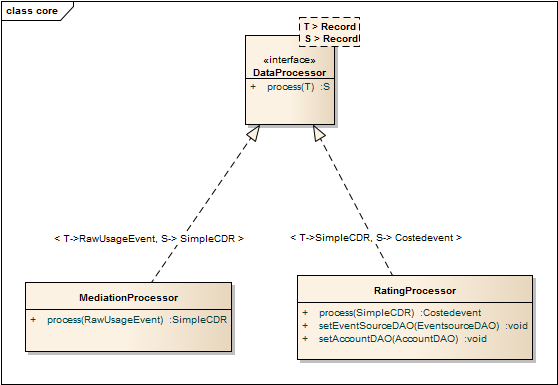
\includegraphics[width=\textwidth]{ch4_business_services}
	\caption{Business services}
	\label{fig:ch4_business_services}
\end{figure}

\subsubsection{Integration Layer}

The integration layer implements the different integration styles of the two prototypes. The batch prototype uses a batch layer which provides components for file-based data integration, transaction and control of batch processes.

The messaging prototype uses a messaging middleware for exchanging messages (see Figure \ref{fig:ch4_messaging_integration}). The messaging middleware provides components for the transport, transformation and routing of messages.

\begin{figure}[htbp]
	\centering
	\subfloat[Batch integration]{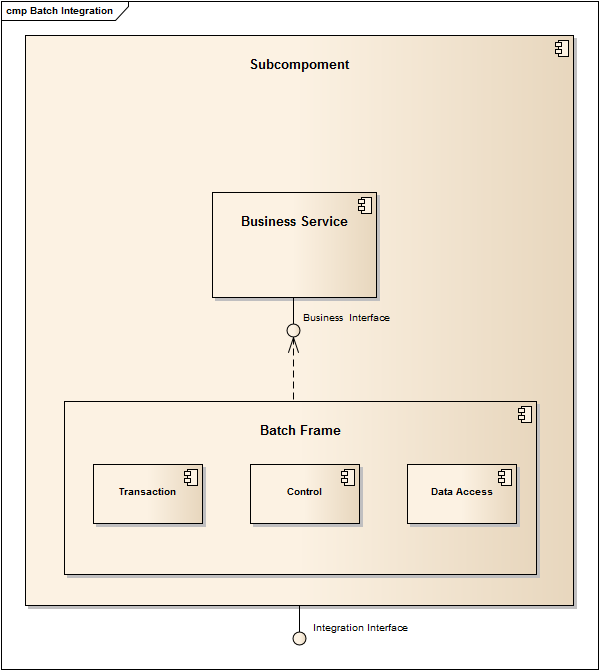
\includegraphics[width=0.4\textwidth]{ch4_batch_integration}\label{fig:ch4_batch_integration}}
	\qquad
	\subfloat[Message-based integration]{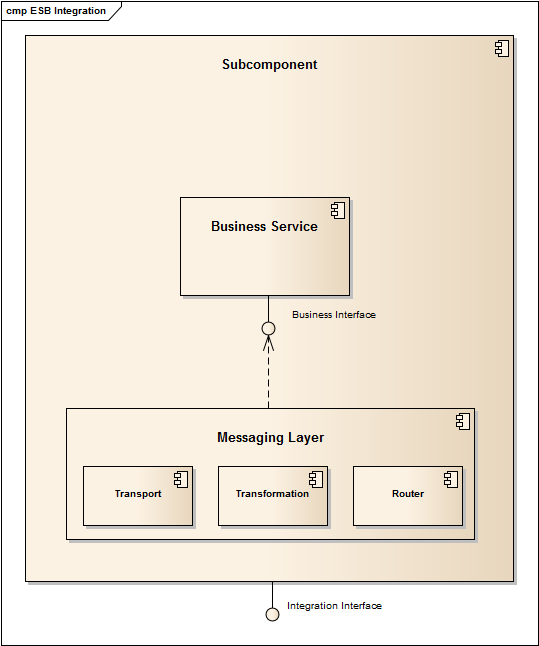
\includegraphics[width=0.4\textwidth]{ch4_messaging_integration}\label{fig:ch4_messaging_integration}}
	\caption{The prototypes use different integration layers.}
\end{figure}

\subsubsection{Data model}
The prototypes use a common data model as shown in Figure \ref{fig:ch4_data_model}. It consists of the following entities:

\begin{itemize}
	\item \textbf{Customer}\\
	Represents a customer. A customer has an account and one or many products.
	\item \textbf{Account}\\
	Contains payment informations of a customer.
	\item \textbf{Product}\\
	A product such as a voice or data plan.
	\item \textbf{Tariff}\\
	The tariff of a product. Defines the price of a product.
	\item \textbf{EventSource}\\
	Mobile number or IP associated with a product instance of a customer.
	\item \textbf{CostedEvent}\\
	An event that has been rated by the rating component.
	\item \textbf{SkippedEvent}\\
	An event that has been skipped by the mediation component. For example a flat rate event.
	\item \textbf{CustomerProduct}\\
	Contains the booked products of a customer. A customer can have zero or many products.
	\item \textbf{CustomerProductTariff}\\
	Contains the tariffs of a product. A product can have one or many tariffs.
\end{itemize}

\begin{figure}[htbp]
	\centering
	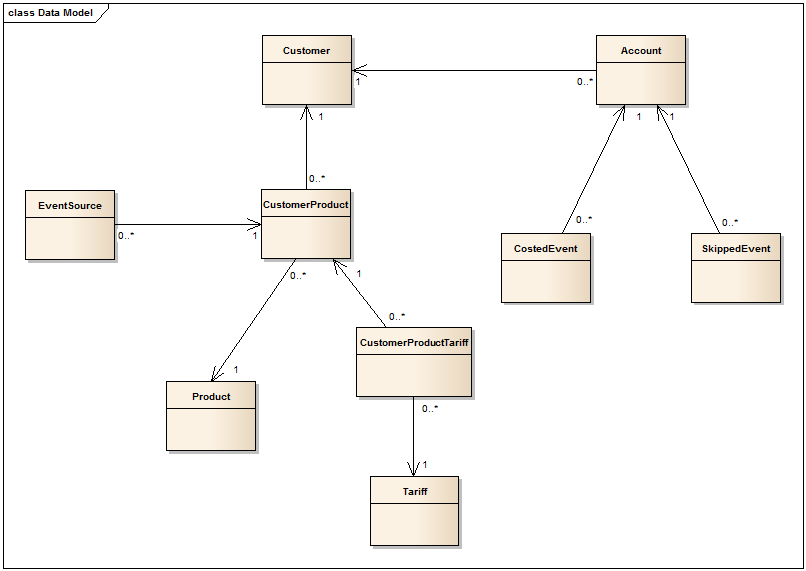
\includegraphics[width=\columnwidth]{ch4_logical_datamodel}
	\caption{Logical data model of the prototype}
	\label{fig:ch4_data_model}
\end{figure}

\subsubsection{Data Access Layer}

The data access layer provides common access to the database by using the \ac{ORM} framework OpenJPA. All business domain entities have been generated from the data model using the toolchain provided by OpenJPA. The data access for retrieving, creating and update of the domain entities is implemented using the DAO pattern \citep{Alur:2003:CJP:863711}.

\subsection{Batch prototype}
The batch prototype implements the billing application utilizing the batch processing type. It uses the Spring Batch framework \citep{springbatch}, a Java framework that facilitates the implementation of batch applications by providing basic building blocks for reading, writing and processing data.

Figure \ref{fig:ch4_batch_prototype} shows the architecture of the batch prototype. It consists of two nodes, mediation batch and rating batch, each implemented as a separate spring batch application. The nodes are integrated using Apache Camel \citep{apachecamel}, an Java integration framework based on enterprise integration patterns, as described by \cite{Hohpe:2003fk}. Apache Camel is responsible for listening on the file system, calling the Spring batch application when a file arrives and transferring the output from the mediation batch node to the rating batch node using \ac{FTP}.

\begin{figure}[htbp]
	\centering
	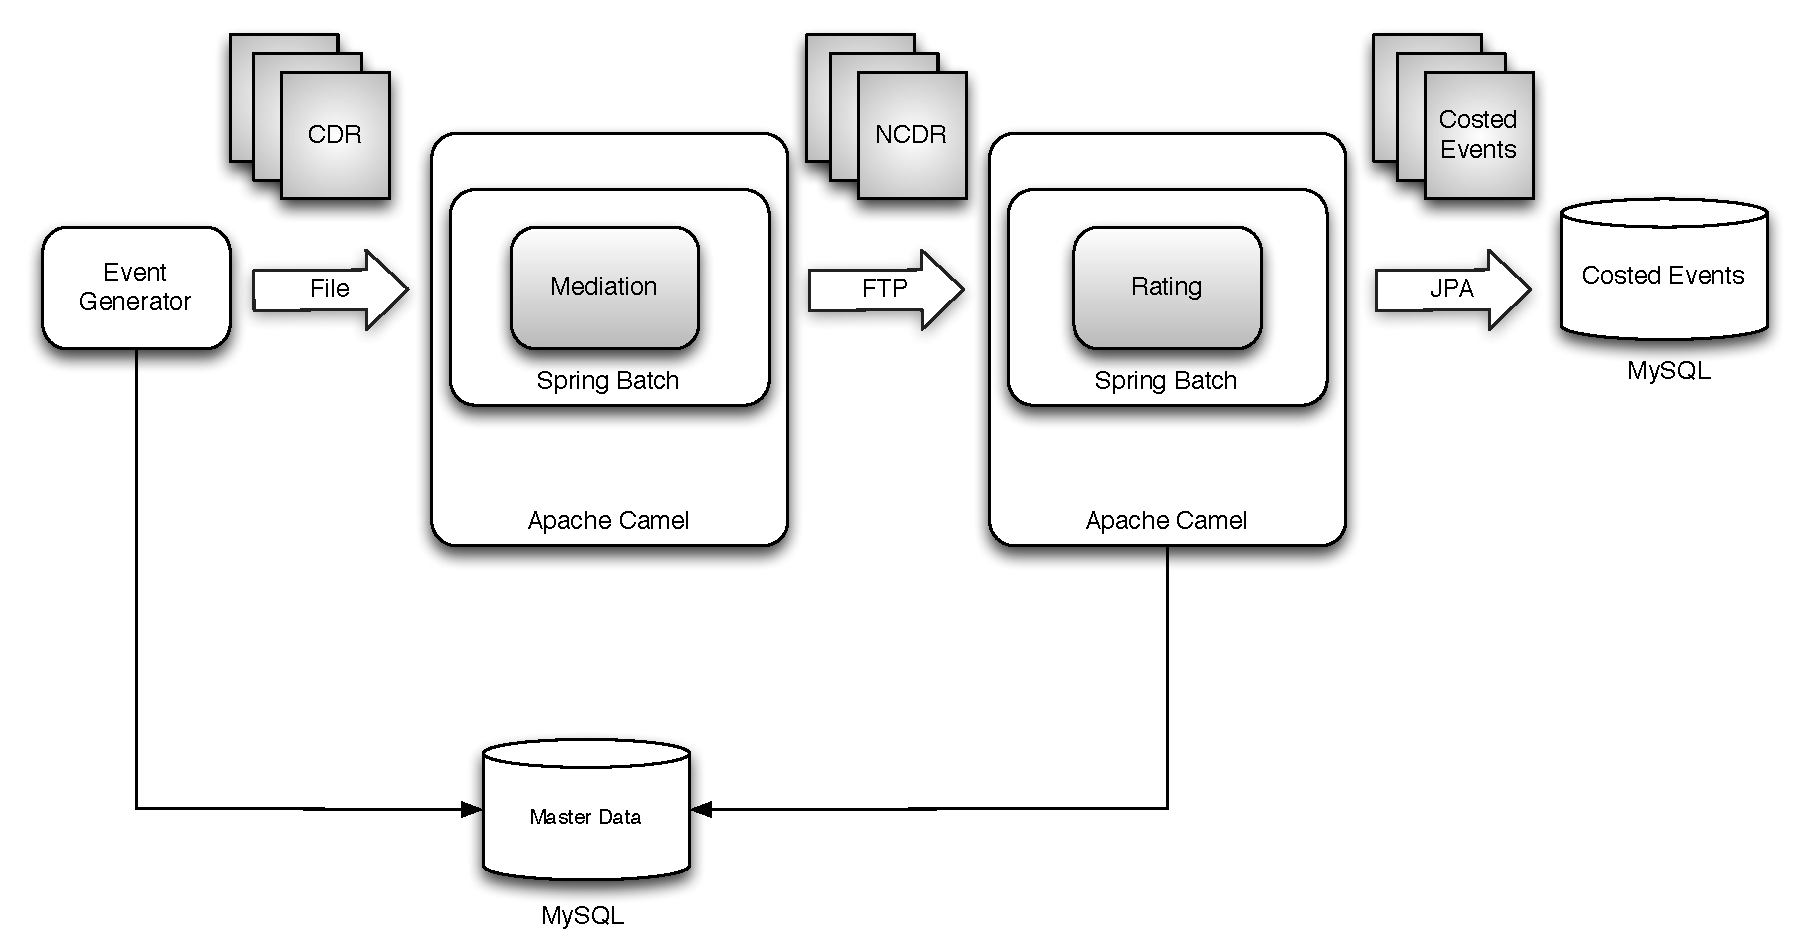
\includegraphics[width=\columnwidth]{batch_prototype}
	\caption{Batch prototype}
	\label{fig:ch4_batch_prototype}
\end{figure}

The batch prototype performs the following steps:
\begin{enumerate}
	\item The \emph{Event generator} generates call detail records and writes them to a single file.
	\item The \emph{Mediation component} opens the file, processes it and writes the output to a single output file. The output file is getting transfered using \ac{FTP} to the \emph{Rating component}.
	\item The \emph{Rating component} opens the file, processes it and writes the costed events to the costed event database.
\end{enumerate}

\subsubsection{Implementation details}
The main entities in Spring Batch are Jobs and Steps. A Job defines the processing flow of the batch application and consists of one or more steps. A basic step is comprised of an item reader, item processor and item writer (see Figure \ref{fig:ch4_spring_batch_step}). 
\begin{figure}[htbp]
	\centering
	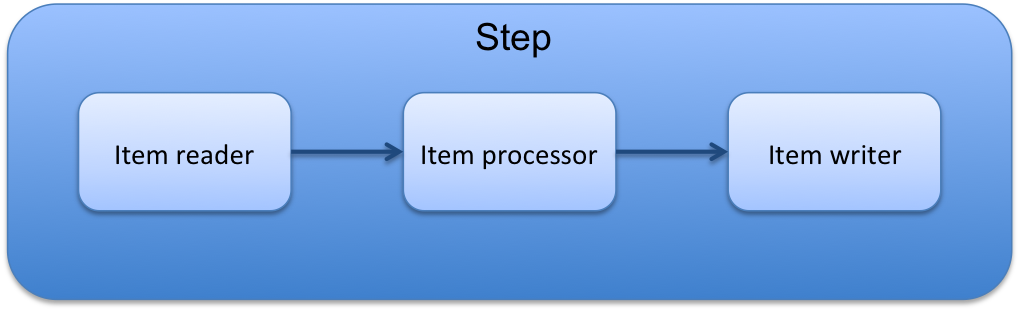
\includegraphics[width=\columnwidth]{spring_batch_step}
	\caption{A Step consists of an item reader, item processor and item writer}
	\label{fig:ch4_spring_batch_step}
\end{figure}

The item reader reads records of data in chunks, for example from a file, and converts them to objects. These objects are then processed by the item processor, which contains the business logic of the batch application. Finally, the processed objects are getting written to the output destination, for example a database, by the item writer.

\lstinputlisting[caption={Mediation batch job definition},label=listing:ch4_mediation_job]{listings/mediation_job.xml}

Listing \ref{listing:ch4_mediation_job} shows the definition of the mediation batch job \emph{mediationMultiThreadedJob}. It consists of two steps, the \emph{mediationMultiThreadedStep} (line 2) and the \emph{renameFileMultiThreadedStep} (line 10). The step \emph{mediationMultiThreadedStep} is multithreaded and uses 10 threads for processing. It consists of a \emph{rawUsageMultiThreadedEventReader} (line 6), a thread safe reader implementation that reads call detail records from the input file and converts them to objects, a \emph{rawUsageEventProcessor}, that processes the call detail objects by calling the mediation business logic and a \emph{loggingSimpleCdrWriter} (line 7), which writes the processed call detail objects to the output file. The step uses an commit interval of 1000, meaning that the input data is processed in chunks of 1000 records. After the input file has been processed by the \emph{mediationMultiThreadedStep} it is getting renamed to its final name by the \emph{renameFileMultiThreadedStep} (line 10).

The mediation batch job is integrated using Apache Camel. Listing \ref{listing:ch4_mediation_route} shows the definition of the mediation batch route.

\begin{lstlisting}[caption={Mediation batch route definition},label=listing:ch4_mediation_route]
public void configure() {
	from("file:data/input")
	.to("spring-batch:mediationMultiThreadedJob?jobLauncherRef=jobLauncher");
        
	from("file:data/output)
	.to("ftp://billing@localhost/src/data?password=billing");
}
\end{lstlisting}

It consists of two routes, the first route listens on the file system for incoming files (line 2) and calls the mediation batch job, when a file arrives (line 3). The second route transfers the output file of the mediation batch job to the rating batch node using \ac{FTP} (line 5-6).

Listing \ref{listing:ch4_rating_job} shows the definition of the rating batch job \emph{ratingMultiThreadedJob}. It consists of a single step \emph{ratingMultiThreadedStep} (line 2), which is comprised of a \emph{simpleCdrMultiThreadedItemReader}, which reads the normalized call detail records written by the mediation batch node, a \emph{simpleCdrProcessor}, that processes the normalized call detail records by calling the rating business logic and a \emph{costedEventWriter}, which writes the processed costed events to the Costed Events database (line 4).

\lstinputlisting[caption={Rating batch job definition},label=listing:ch4_rating_job]{listings/rating_job.xml}

\subsection{Messaging prototype}

The messaging prototype implements the billing prototype utilizing the message-oriented processing type. It uses Apache Camel \citep{apachecamel} as the messaging middleware.

Figure \ref{fig:ch4_messaging_prototype} shows the architecture of the messaging prototype. It consists of three nodes, the billing route, mediation service and rating service. The billing route implements the main flow of the application. It is responsible for reading messages from the billing queue, extracting the payload, calling the mediation and rating service and writing the processed messages to the database. The mediation service is a webservice representing the mediation component. It is a SOAP service implemented using Apache CXF and runs inside an Apache Tomcat container. The same applies to the rating service, representing the rating component.

\begin{figure}[htbp]
	\centering
	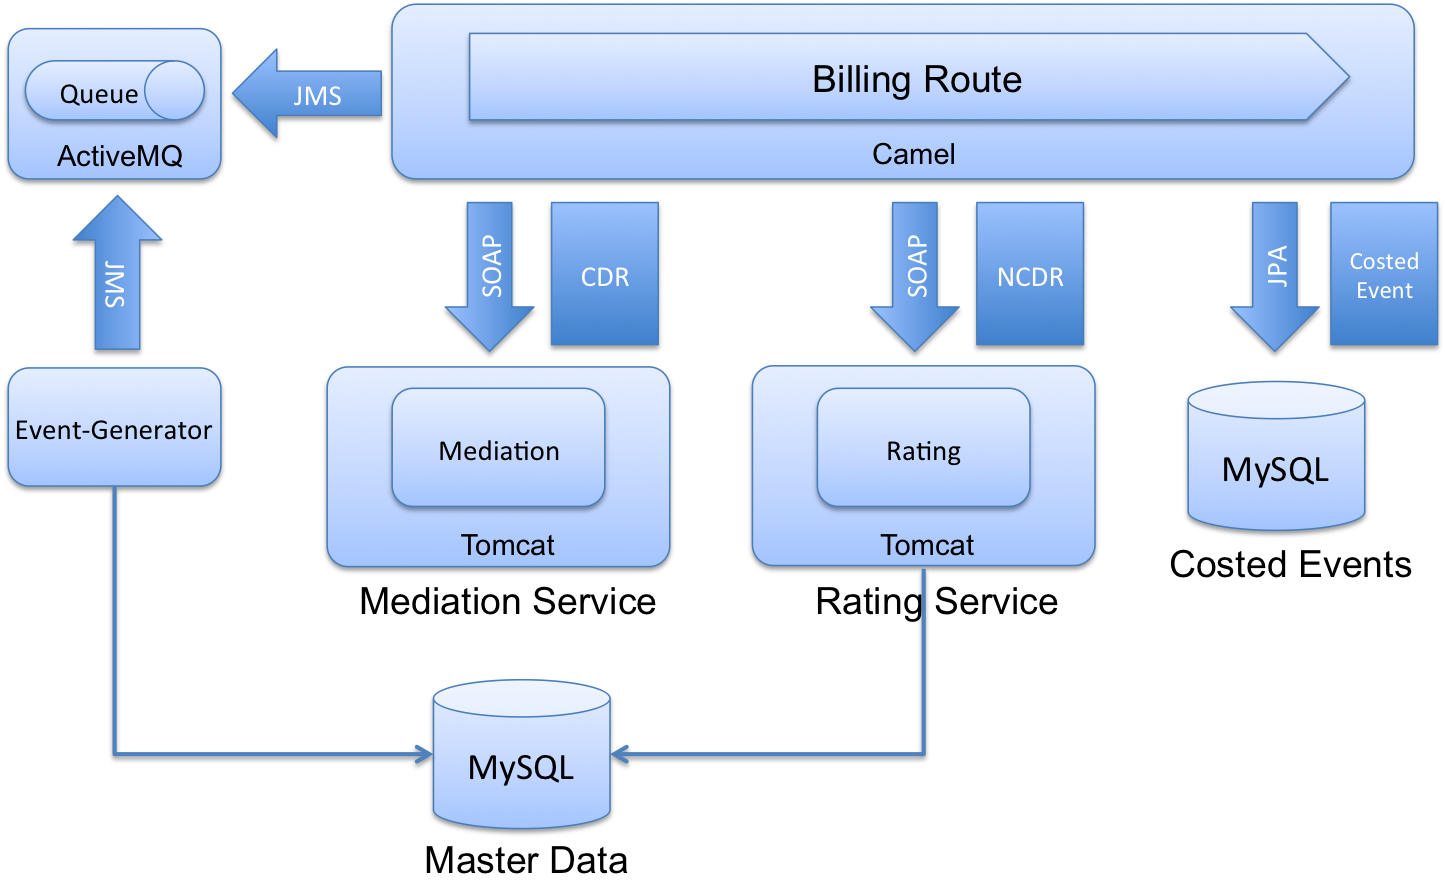
\includegraphics[width=\columnwidth]{messaging_prototype}
	\caption{Message-based prototype}
	\label{fig:ch4_messaging_prototype}
\end{figure}

Listing \ref{listing:ch4_billing_route} shows the definition of the billing route using the Apache Camel fluent \ac{API}.
The billing route performs the following steps:

\begin{enumerate}
	\item The message is read from the billing queue using \ac{JMS} (line 5). The queue ist hosted by an Apache ActiveMQ instance.
	\item The message is unmarshalled using \ac{JAXB} (line 6).
	\item The \emph{Mediation service} is called by the CXF Endpoint of the billing route (line 7)
	\item The response of the \emph{Mediation webservice}, the normalized call detail record, is unmarshalled (line 8). 
	\item The \emph{Rating service} is called by the CXF Endpoint of the billing route (line 9).
	\item The response of the \emph{Rating webservice}, that is the costed event, is unmarshalled (line 10).
	\item The costed event is written to the \emph{Costed Events} DB (line 11).
\end{enumerate}

If an error occurs during the processsing of an event, it is written to an error \ac{JMS} queue (line 3).

\begin{lstlisting}[caption={Billing route definition},label=listing:ch4_billing_route]
public void configure() {
		
	errorHandler(deadLetterChannel("activemq:queue:BILLING.ERRORS"));
	
	from("activemq:queue:BILLING.USAGE_EVENTS")
		.unmarshal("jaxbContext")
		.to("cxf:bean:mediationEndpoint?dataFormat=POJO&defaultOperationName=processEvent")
		.process(new ProcessEventPostProcessor())
		.to("cxf:bean:ratingEndpoint?dataFormat=POJO&defaultOperationName=processCallDetail")
		.process(new ProcessCallDetailPostProcessor())
		.process(costedEventProcessor);
}
\end{lstlisting}

\section{Performance evaluation}\label{sec:ch4_evaluation}
To compare the performance characterics of the two processing types, batch processing and message-based processing, a performance evaluation has been conducted with the main focus on latency and throughput.

This section describes the approach and the results of the performance evaluation.

\subsection{Measuring points}
A number of measuring points have been defined for each prototype by breaking down the processing in single steps and assigning a measuring point to each step. Figure \ref{fig:ch4_measuring_points_batch} and \ref{fig:ch4_measuring_points_messaging} show the measuring points of the batch prototype and the messaging prototype. 

\begin{figure}[htpb]
	\centering
	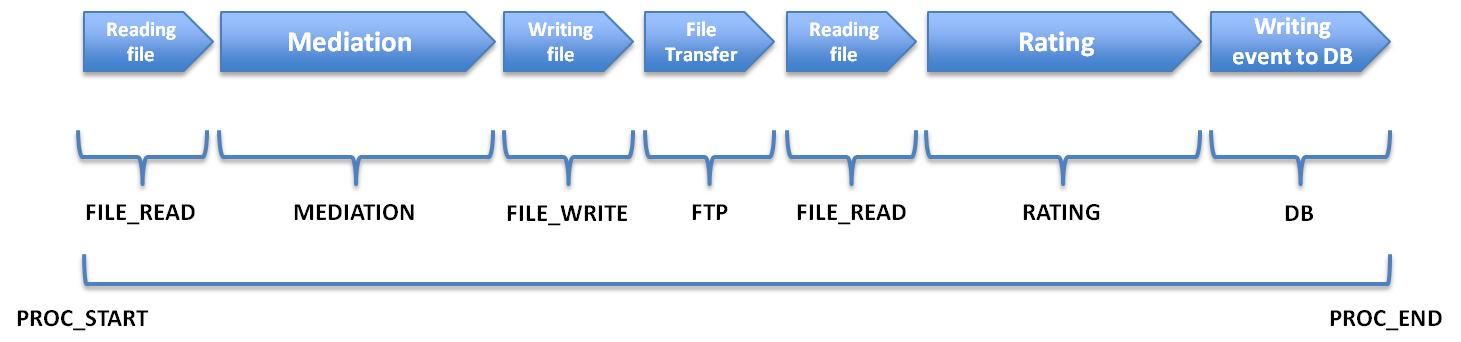
\includegraphics[width=\columnwidth]{measuring_points_batch}
	\caption{Measuring points of the batch prototye}
	\label{fig:ch4_measuring_points_batch}
\end{figure}

\begin{figure}[htpb]
	\centering
	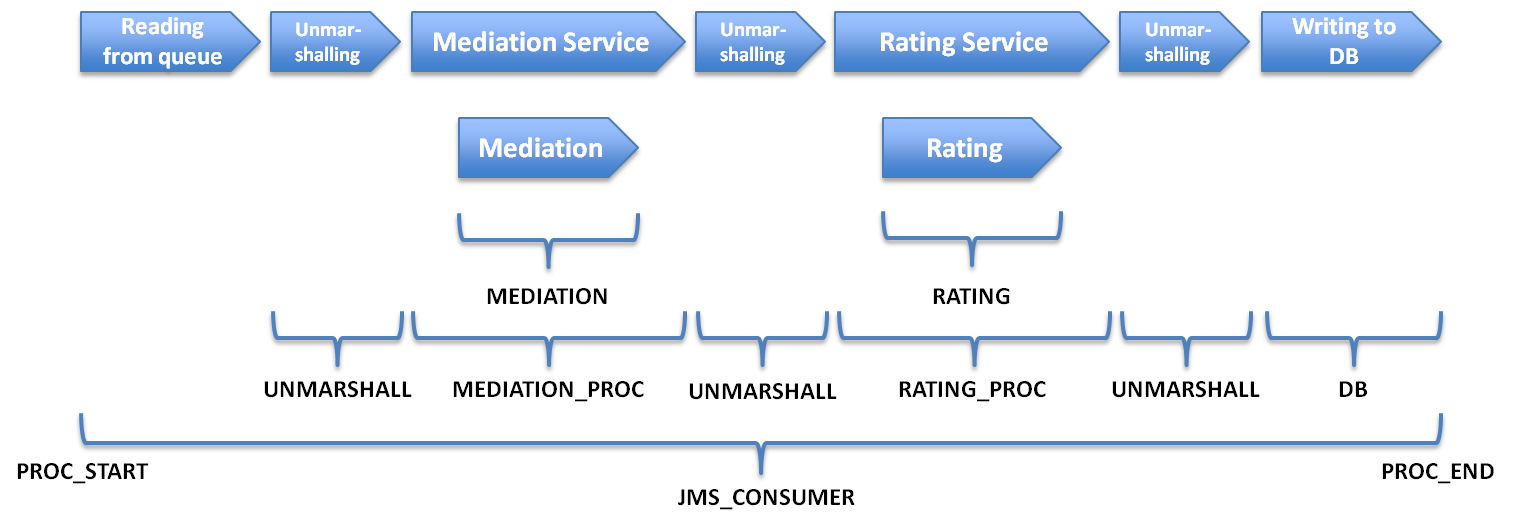
\includegraphics[width=\columnwidth]{measuring_points_messaging}
	\caption{Measuring points of the messaging prototype}
	\label{fig:ch4_measuring_points_messaging}
\end{figure}

A detailed description of each point is shown in Table \ref{table:ch4_measuring_points_batch} and \ref{table:ch4_measuring_points_messaging}.

\begin{table}
	%\renewcommand{\arraystretch}{1.3}
	\centering
	\begin{tabularx}{\textwidth}{@{} l X @{}}
		\caption{Measuring points of the batch prototype} \label{table:ch4_measuring_points_batch}\\
		\toprule
		\bfseries Measuring point & \bfseries Description\\
		\midrule
		PROC\_START & Timestamp denoting the start of processing an event\\
		\midrule
		PROC\_END & Timestamp denoting the end of processing an event\\
		\midrule
		FILE\_READ & Elapsed time for reading events from file\\
		\midrule
		MEDIATION & Elapsed time used by the mediation component\\
		\midrule
		FILE\_WRITE & Elapsed time for writing events to file\\
		\midrule
		FTP & Elapsed time for file transfer using FTP\\
		\midrule
		RATING & Elapsed time used by the rating component\\
		\midrule
		DB & Elapsed time for writing event to the database\\
		\bottomrule 
	\end{tabularx}
\end{table}

\begin{table}[htpb]
	\centering
	\begin{tabularx}{\textwidth}{@{} l X @{}}
		\caption{Measuring points of the messaging prototype} \label{table:ch4_measuring_points_messaging}\\
		\toprule
		\bfseries Measuring point & \bfseries Description\\
		\midrule
		PROC\_START & Timestamp denoting the start of processing an event\\
		\midrule
		PROC\_END & Timestamp denoting the end of processing an event\\
		\midrule
		JMS\_CONSUMER & Elapsed time processing a single event\\
		\midrule
		UNMARSHALL & Elapsed time for unmarshalling an event\\
		\midrule
		MEDIATION\_PROC & Elapsed time needed for calling the mediation service\\
		\midrule
		MEDIATION & Elapsed time used by the mediation component\\
		\midrule
		RATING\_PROC & Elapsed time needed for calling the rating service\\
		\midrule
		RATING & Elapsed time used by the rating component\\
		\midrule
		DB & Elapsed time for writing event to the database\\
		\bottomrule 
	\end{tabularx}
\end{table}

\subsection{Instrumentation}
A logging statement for each measuring point has been added at the appropriate code location of the prototypes using different techniques.

\begin{enumerate}
	\item \textbf{Directly in the code}\\Whenever possible, the logging statements have been inserted directly in the code. This has been the case, when the code that should be measured, has been written exclusively for the protoype, for example the mediation and rating components.
	\item \textbf{Delegation}\\When the code to instrument has been part of a framework that is configurable using Spring, an instrumented delegate has been used.
	\item \textbf{AOP}\\Finally, when the code that should get instrumented was part of a framework that was not configurable using Spring, the logging statements have been added using aspects, which are woven into the resulting class files using AspectJ.
\end{enumerate}

\subsection{Test environment}
\label{sec:ch4_test_environment}

The two prototypes have been deployed to an Amazon EC2 environment to conduct the performance evaluation, with the characterics described in Table \ref{table:ch4_amazon_ec2}.

\subsubsection{Batch prototype}

The batch prototype comprises two EC2 nodes, the \emph{Mediation Node} and the \emph{Rating Node}, containing the \emph{Mediation Batch} and the \emph{Rating Batch}, respectively. The \emph{Costed Event Database} is hosted on the \emph{Rating Node} as well. Figure \ref{fig:ch4_batch_deployment_model} shows the deployment diagramm of the Batch prototype.

\begin{figure}[htbp]
	\centering
	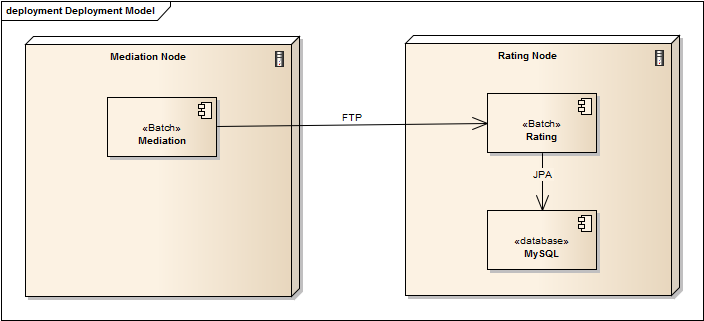
\includegraphics[width=\columnwidth]{batch_deployment_model}
	\caption{Batch prototype deployment on EC2 instances}
	\label{fig:ch4_batch_deployment_model}
\end{figure}

\subsubsection{Messaging Prototype}

The messaging prototype consists of three EC2 nodes, as shown in Figure \ref{fig:ch4_messaging_deployment_model}. The \emph{Master Node} hosts the \emph{ActiveMQ Server} which runs the JMS queue containining the billing events, the \emph{Billing Route}, which implements the processing flow of the prototype and the \emph{MySQL Database} containing the \emph{Costed Event Database}. The \emph{Mediation Node} and \emph{Rating Node} are containing the \emph{Mediation Service} and \emph{Rating Service}, respectively, with each service running inside an Apache Tomcat container.

\subsection{Clock Synchronization}

The clocks of the \emph{Mediation Node} and \emph{Rating Node} are synchronized with the clock of the \emph{Master Node} using PTPd \citep{ptpd}, an implementation of the \ac{PTP} \citep{IEEE_PTP}. The clock of the \emph{Master Node} itself is synchronised with a public timeserver using the \ac{NTP}. Using this approach, a sub-millisecond precision is achieved.

\begin{figure}[htbp]
	\centering
	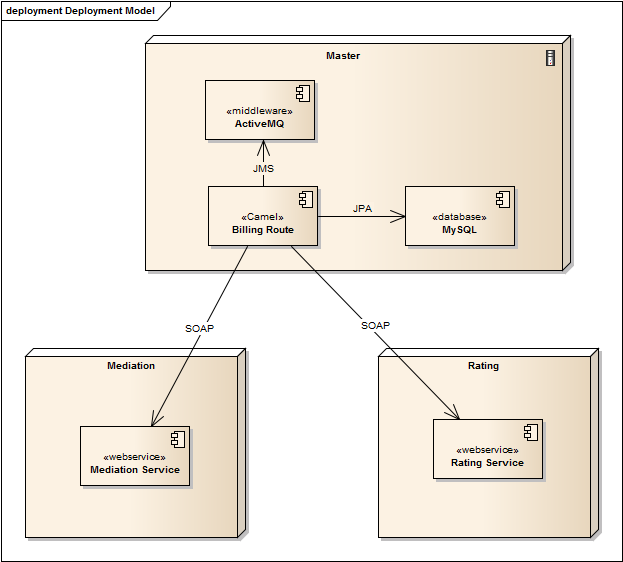
\includegraphics[width=\columnwidth]{messaging_deployment_model}
	\caption{Messaging prototype deployment on EC2 instances}
	\label{fig:ch4_messaging_deployment_model}
\end{figure}

\begin{table}[htbp]
	\centering
	\begin{tabularx}{\textwidth}{@{} l X @{}}
		\caption{Amazon EC2 instance configuration} \label{table:ch4_amazon_ec2} \\
		\toprule
		\bfseries Instance type & M1 Extra Large (EBS optimized)\\
		\midrule
		\bfseries Memory & 15 GiB\\
		\midrule
		\bfseries Virtual Cores & 8 (4 cores x 2 units)\\
		\midrule
		\bfseries Architecture & 64-bit\\
		\midrule
		\bfseries EBS Volume & 10 GiB (100 IOPS)\\
		\midrule
		\bfseries Instance Store Volumes & 1690 GB (4x420 GB Raid 0)\\
		\midrule
		\bfseries Operating System & Ubuntu 12.04 LTS\\
		& (GNU/Linux 3.2.0-25-virtual x86\_64)\\
		\midrule 
		\bfseries Database & MySQL 5.5.24\\
		\midrule
		\bfseries Messaging Middleware & Apache ActiveMQ 5.6.0\\
		\bottomrule
	\end{tabularx}
\end{table}

\subsection{Preparation and execution of the performance tests}
For running the performance tests, the Master Data DB has been set up with a list of customers, accounts, products and tariffs with each prototype using the same database and data. While part of the testdata like the products and tariffs have been created manually, the relationship between the customers and the products have been generated by a test data generator.
\newpage
After setting up the master data, a number of test runs have been executed using different sizes of test data (1.000, 5.000, 10.000, 50.000, 100.000, 500.000, 1.000.000 records). To get reliable results, each test configuration has been run three times. Out of the three runs for each configuration, the run having the median processing time has been used for the evaluation.

For each test run, the following steps have been executed:
\begin{enumerate}
	\item \textbf{Generating test data}\\In case of the batch prototype, the event generator writes the test data to file. In case of the messaging prototype, the event generator writes the test data to a \ac{JMS} queue.
	\item \textbf{Running the test}\\Each prototype listens on the file system and the \ac{JMS} queue, respectively. Using the batch prototype, the processing starts when the input file is copied to the input folder of the mediation batch application by the event genarotor. Using the messaging prototype, the processing starts when the first event is written to the JMS queue by the test generator.
	\item \textbf{Validating the results}\\Processsing the log files written during the test run
	\item \textbf{Cleaning up}\\Deleting the created costed events from the DB.
\end{enumerate}

Before running the tests, each prototype has been warmed up by processing 10.000 records.

\subsection{Results} \label{sec:ch4_results}
The performance evaluation yields the following results.

\subsubsection{Throughput}

The throughput per second for a test run with $N$ records is defined as
\begin{displaymath}
{TP/s}_N = N / PT_N
\end{displaymath}
with $PT_N$ being the total processing time for $N$ records. 
Figure \ref{fig:ch4_result_throughput} shows the measured throughput of the batch and messaging prototypes. The messaging prototype is able to process about 70 events per second. The maximum throughput of the batch prototype is about 383 records per second which is reached with an input of 1.000.000 records.

\begin{figure}[htbp]
	\centering
	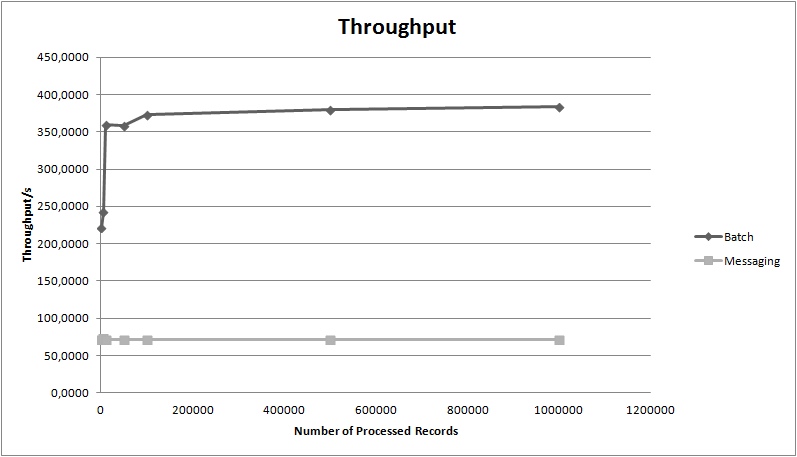
\includegraphics[width=\columnwidth]{throughput_result}
	\caption{Throughput}
	\label{fig:ch4_result_throughput}
\end{figure}

\subsubsection{Latency}\label{sec:result_latency}

Figure \ref{fig:ch4_result_latency} shows the measured latencies of the batch and messaging prototypes. To rule out peaks, the 95th percentile has been used, that is, 95\% of the measured latencies are below this value. In case of the batch prototype, the 95th percentile latency is a linear function of the amount of data. The latency increases proportionally to the number of processd records. In case of the messaging prototype, the 95th percentile latency is approximately a constant value which is independant of the number of processed records.

\begin{figure}[htbp]
	\centering
	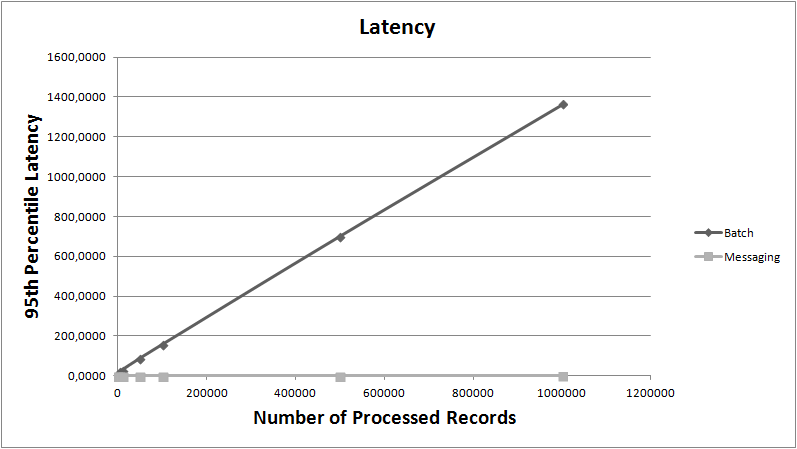
\includegraphics[width=\columnwidth]{latency_result}
	\caption{Latency}
	\label{fig:ch4_result_latency}
\end{figure}

\subsubsection{Processing overhead}

The overhead of the batch prototype is about 7\% of the total processing time, independant of the number of processed records, as shown in Figure \ref{fig:ch4_overhead_batch}. This overhead contains file operations, such as opening, reading, writing and closing of input files, the file transfer between the Mediation and Rating Nodes and the database transactions to write the the processed event to the Costed Events DB.

\begin{figure}[htbp]
	\centering
	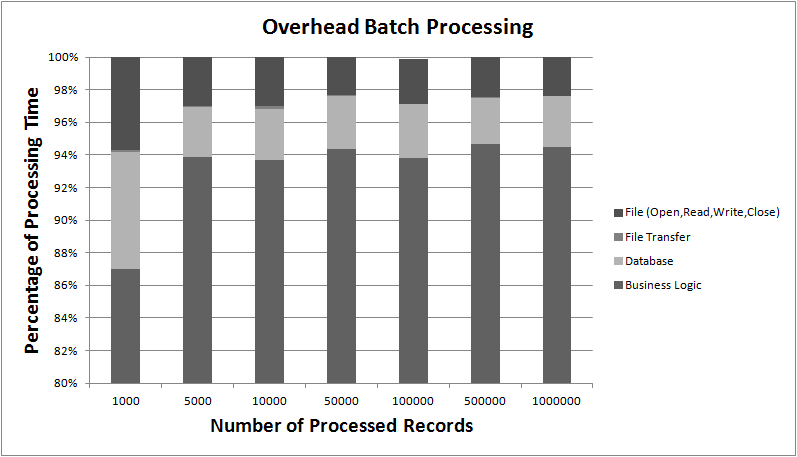
\includegraphics[width=\columnwidth]{overhead_batch}
	\caption{Overhead batch prototype}
	\label{fig:ch4_overhead_batch}
\end{figure}

On the contrary, the overhead of the messaging prototype is about 84\% of the total processing time (see Figure \ref{fig:ch4_overhead_messaging}). In case of the messaging prototype, the overhead contains the JMS overhead, that is the overhead for reading events from the message queue, the webservice overhead needed for calling the Mediation and Rating services including marshalling and unmarshalling of input data and the overhead caused the database transactions to write the processed events to the Costed Events DB. Most of the overhead is induced by the webservice overhead and the database overhead. Since every event is written to the database in its own transaction, the database overhead of the messaging prototype is much larger than the database overhead of the batch prototype.

\begin{figure}[htbp]
	\centering
	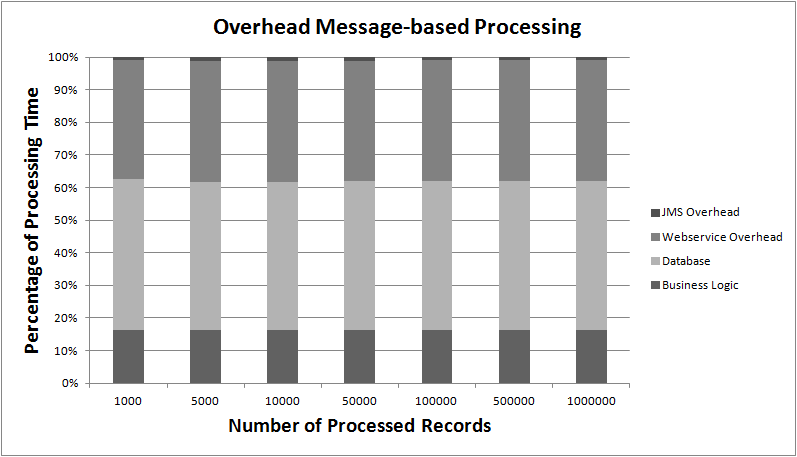
\includegraphics[width=\columnwidth]{overhead_messaging}
	\caption{Overhead messaging prototype}
	\label{fig:ch4_overhead_messaging}
\end{figure}

\subsubsection{System utilisation}

\begin{figure}[htbp]
	\centering
	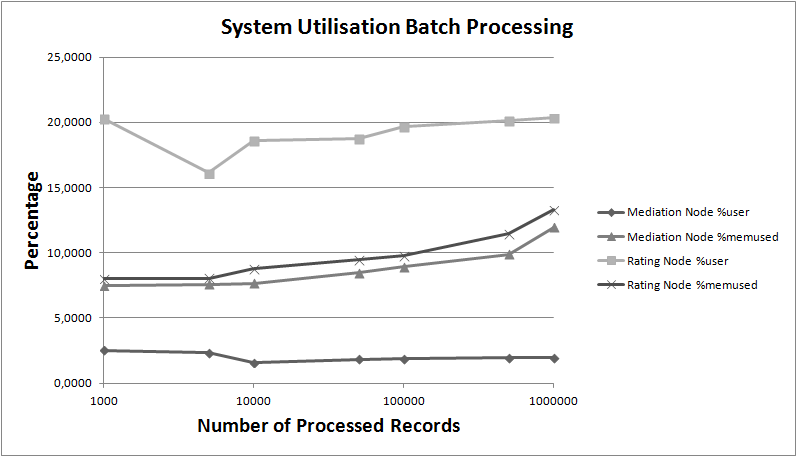
\includegraphics[width=\columnwidth]{systemutilisation_batch}
	\caption{System utilisation batch prototype}
	\label{fig:ch4_systemutilisation_batch}
\end{figure}

The system utilisation has been measured using the sar (System Activity Report) command while running the performance tests. Figure \ref{fig:ch4_systemutilisation_batch} shows the mean percentage of CPU consumption at the user level (\%user) and the mean percentage of used memory (\%memused) for the Mediation node and Rating node of the Batch prototype.
The CPU utilisation of Medation Node and Ratig Node is about 2\% and 19\%, respectively. The memory utilisation increases slowly with the number of processed records.

Figure \ref{fig:ch4_systemutilisation_messaging} shows the mean CPU consumption and mean memory usage for the nodes of the Messaging prototype. The CPU utilisation of the Master Node, Mediation Node and Rating Node is about 9\%, 1\% and 6\%, respectively.
As the same with the batch prototye, the memory utilisation of the messaging prototype increases with the number of processed records. The memory utilisation of the master node peaks at about 38\% with 500000 processed records.
With 1000000 processed records, the memory utilisation is only about 25\%, which presumably can be accounted to the garbage collector.

\begin{figure}[htbp]
	\centering
	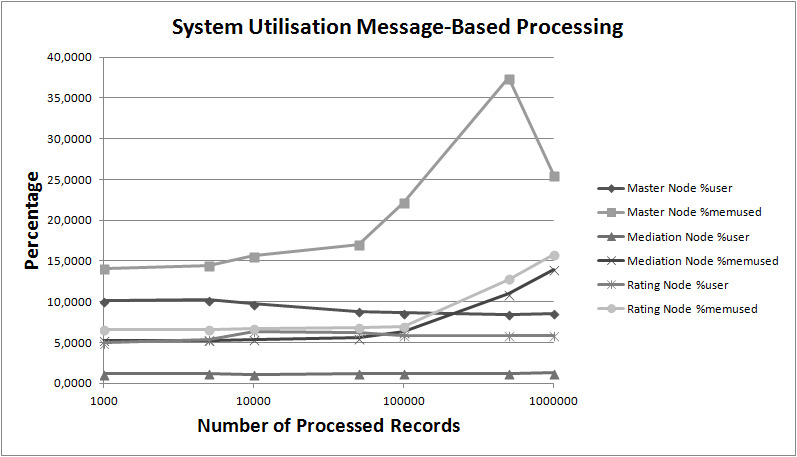
\includegraphics[width=\columnwidth]{systemutilisation_messaging}
	\caption{System utilisation messaging prototype}
	\label{fig:ch4_systemutilisation_messaging}
\end{figure}

\section{Impact of data granularity on throughput and latency}\label{sec:ch4_impact_granularity}
The results presented in Section \ref{sec:ch4_results} suggest that the throughput of the messaging prototype can be increased by increasing the granularity of the data that is beeing processed. Data granularity relates to the amount of data that is processed in a unit of work, for example in a single batch run or an event.
In order to examine this approach, we have repeated the performance tests using different package sizes for processing the data.

\begin{figure}[htbp]
	\centering
	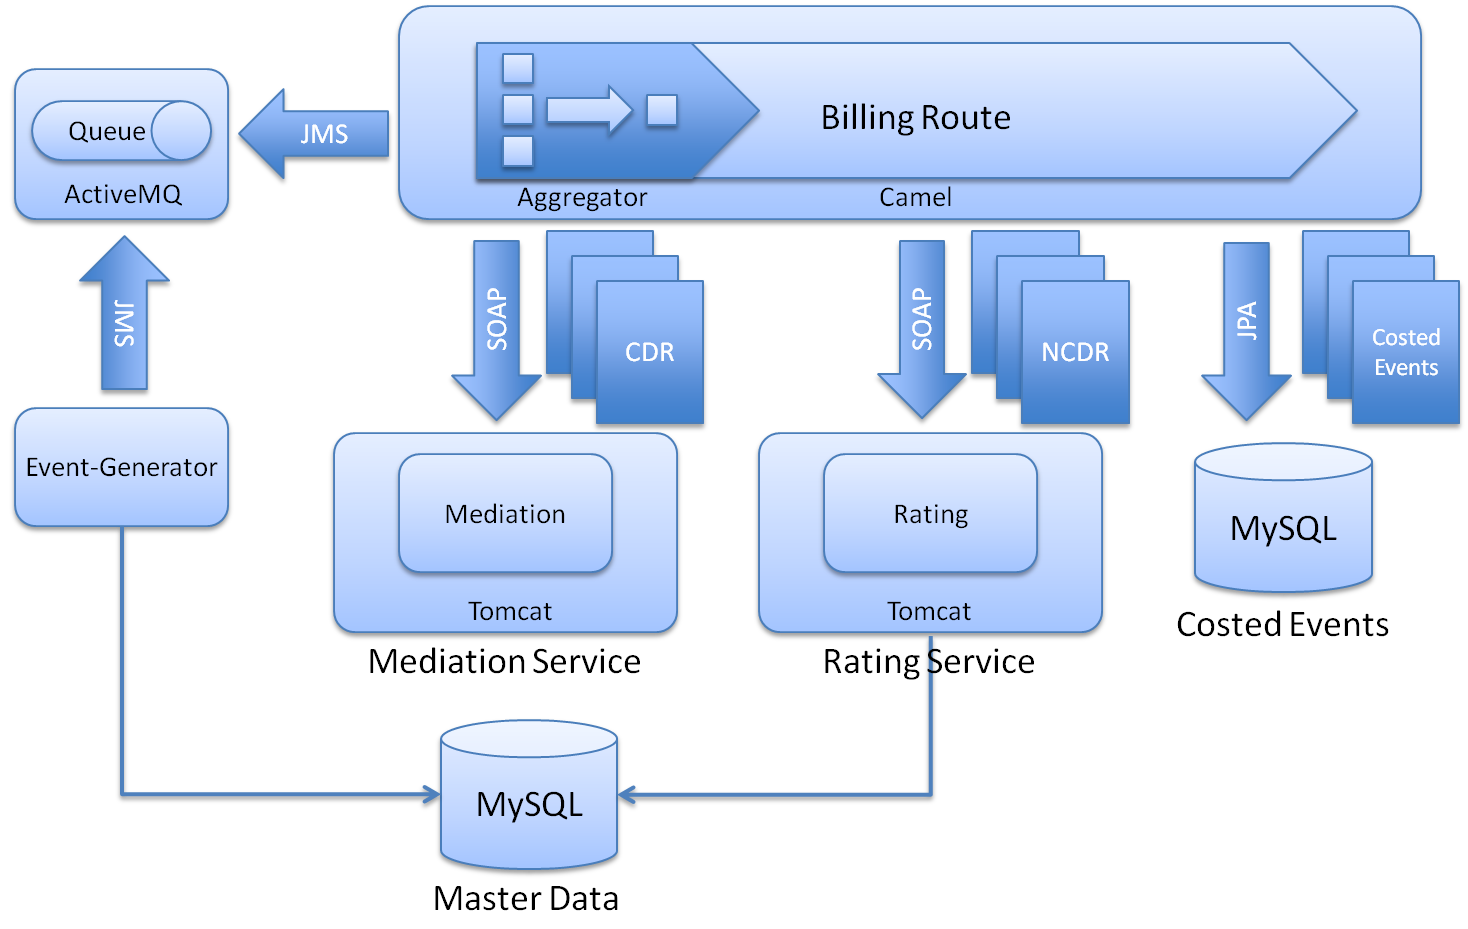
\includegraphics[width=\columnwidth]{messaging_prototype_aggregator}
	\caption{The data granularity is controlled by an aggregator}
	\label{fig:ch4_messaging_prototype_aggregator}
\end{figure}

For this purpose, the messaging prototype has been extended to use an aggregator in the messaging route. The aggregator is a stateful filter which stores correlated messages until a set of messages is complete and sends this set to the next processing stage in the messaging route. In case of the messaging prototype, messages are not corelated to each other and also the messages can be processed in an arbitrary order. A set of messages is complete when it reaches the configured package size. In other scenarios, it is possible to corelate messages by specific data, for example an account number or by a business rule.

Listing \ref{listing:ch4_billing_route_aggregator} shows the definition of the billing route using the aggregator processor, which is provided by Apache Camel (line 7). The aggregator is configured using the correlation expression \lstinline$constant(true)$, which simply aggregates messages in order of their arrival and the aggregation strategy \lstinline$UsageEventsAggrationStrategy$, which implements the merging of incoming messages with already merged messages. The aggregation size is set by \lstinline$completionSize$. The specific value is set in a configuration file. As a fallback, \lstinline$completionTimeout$ defines a timeout in milliseconds to send the set of aggregated messages to the next processing stage before it has reached the defined aggregation size. \lstinline$parallelProcessing$ indicates that the aggregator should use multiple threads (default is 10) to process the finished sets of aggregated messages.

\begin{lstlisting}[caption={Billing route definition with an additional aggregator},label=listing:ch4_billing_route_aggregator]
public void configure() {
		
	errorHandler(deadLetterChannel("activemq:queue:BILLING.ERRORS"));
	
	from("activemq:queue:BILLING.USAGE_EVENTS")
		.unmarshal("jaxbContext")
		.aggregate(constant(true), new UsageEventsAggrationStrategy()).completionSize(completionSize).completionTimeout(completionTimeout).parallelProcessing()
		.to("cxf:bean:mediationEndpoint?dataFormat=POJO&headerFilterStrategy=#dropAllMessageHeadersStrategy&defaultOperationName=processEvents")
		.process(new ProcessEventsPostProcessor())
		.to("cxf:bean:ratingEndpoint?dataFormat=POJO&headerFilterStrategy=#dropAllMessageHeadersStrategy&defaultOperationName=processCallDetails")
		.process(new ProcessCallDetailsPostProcessor())
		.process(costedEventsProcessor);
}
\end{lstlisting}

Figure \ref{fig:ch4_throughput_aggregation} shows the impact of different aggregatation sizes on the throughput of the messaging prototype. For each test 100.000 events have been processed.
\begin{figure}[htbp]
	\centering
	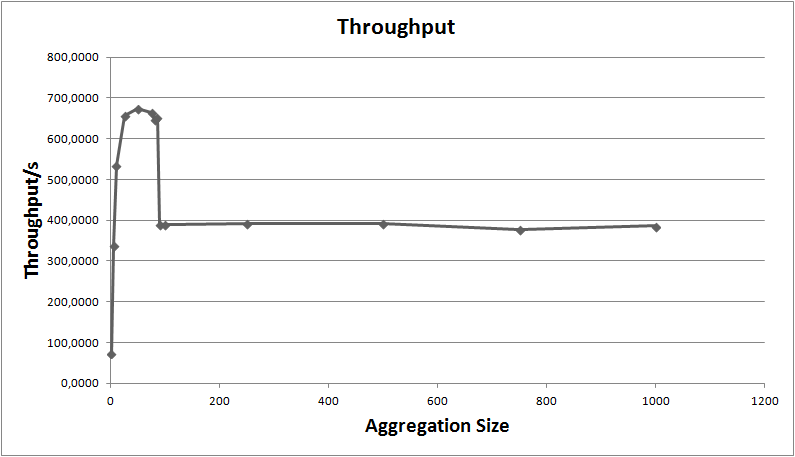
\includegraphics[width=\columnwidth]{throughput_aggregation}
	\caption{Impact of different aggregation sizes on throughput}
	\label{fig:ch4_throughput_aggregation}
\end{figure}
The throughput increases constantly for $1<aggregation\_size<=50$ with a maximum of 673 events per second with $aggregation\_size=50$. Higher aggregation sizes than 50 do not further increase the throughput, it stays around 390 events per second. Surprisingly, the maximum throughput of 673 events per second even outperforms the throughput of the batch prototype which is about 383 records per second. This is presumably a result of the better multithreading capabilities of the camel framework.

Increasing the aggregation size also decreases the processing overhead, as shown in Figure \ref{fig:ch4_overhead_aggregation}. An aggregate size of 10 decreases the overhead by more than 50\% compared to an aggregate size of 1. Of course, the integration of the aggregator adds an additional overhead which is insignificant for $aggregation\_size>50$.
\begin{figure}[htbp]
	\centering
	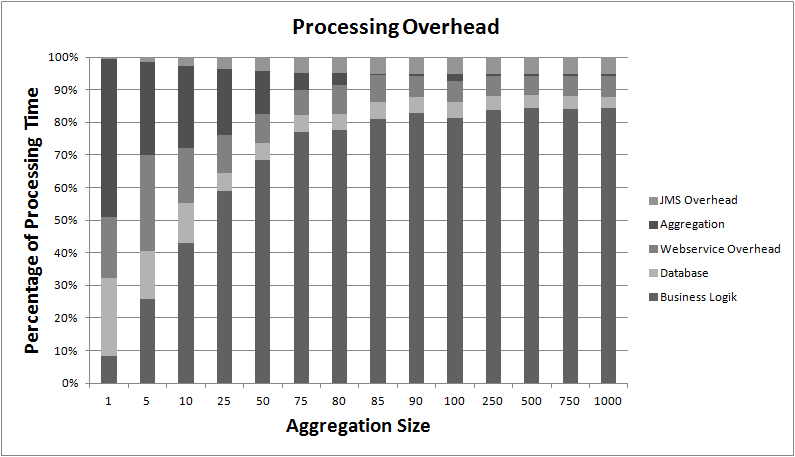
\includegraphics[width=\columnwidth]{overhead_aggregation}
	\caption{Impact of different aggregation sizes on processing overhead}
	\label{fig:ch4_overhead_aggregation}
\end{figure}

The increased throughput achieved by increasing the aggregation size comes with the cost of a higher latency. Figure \ref{fig:ch4_latency_aggregation} shows the impact of different aggregation sizes on the 95th percentile latency of the messaging prototype. 
\begin{figure}[htbp]
	\centering
	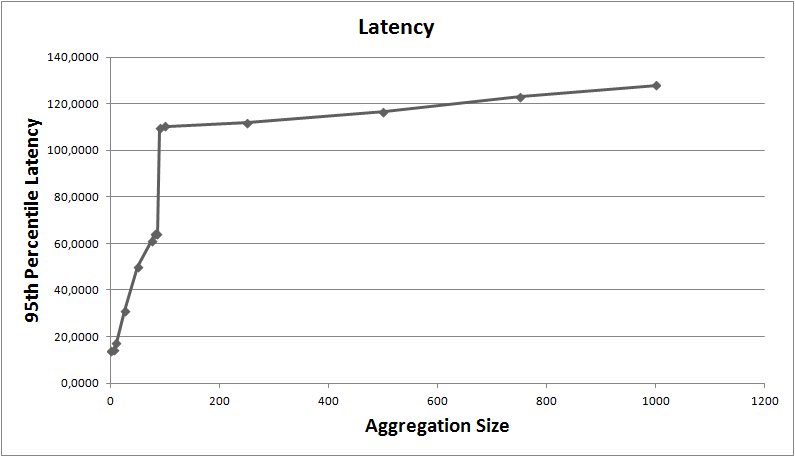
\includegraphics[width=\columnwidth]{latency_aggregation}
	\caption{Impact of different aggregation sizes on latency}
	\label{fig:ch4_latency_aggregation}
\end{figure}

An aggregation size of 50, resulting in the maximum throughput of 673 events per seconds, shows a 95th percentile latency of about 68 seconds. This latency is significantly higher than the latency of the messaging system without message aggregation, which is about 0,15 seconds (see Section \ref{sec:result_latency}).

The results indicate that there is an optimal range for the aggregation size to control the throughput and latency of the system. Setting the aggregation size higher than a certain threshold leads to a throughput drop and latency gain. In case of our prototype, this threshold is between an aggregation size of 85 and 90. The observed throughput drop and latency gain is caused by a congestion in the aggregator. Messages are read faster from the queue than they are getting processed by the aggregator.

Figure \ref{fig:ch4_systemutilisation_aggregation} shows the impact of different aggregation sizes on the system utilisation. The CPU utilisation of the Master node shows a maximum of 30\% with an aggregation size of 25. An $aggregation\_size >= 90$ results in a CPU utilisation of about 15\%. The maximum memory utilisation of the Master node is 41\% with an aggregation size of 100.

The maximum system utilisation of the Rating node is 25\% with an aggregation size of 80. The memory utilisation is between 7-8\% irrespective of aggregation size. Maximum system and memory utilisation of the Mediation node are also irrespective of aggregation size, beeing less than 2\% and 8\%, respectively.

\begin{figure}[htbp]
	\centering
	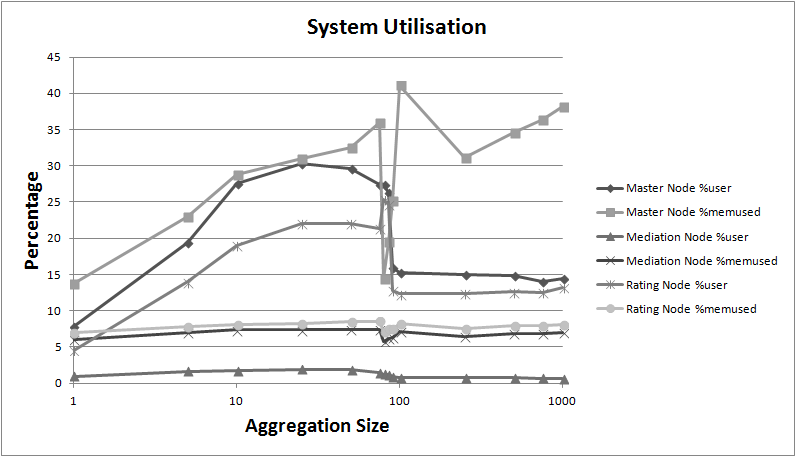
\includegraphics[width=\columnwidth]{systemutilisation_aggregation}
	\caption{Impact of different aggregation sizes on system utilisation}
	\label{fig:ch4_systemutilisation_aggregation}
\end{figure}

When using high levels of data granularity, the messaging system is essentially a batch processing system, providing high throughput with high latency. To provide near-time processing an optimum level of data granularity would allow having the lowest possible latency with the lowest acceptable throughput.

\section{Discussion with respect to related work}\label{sec:ch4_related_work}
This section gives an overview of work related to the performance evaluation of batch and message-based systems presented in this chapter and discusses the approach that has been taken. 

Related work can be categorised in two different topics, performance measuring and performance prediction. 
Performance measuring is applied to evaluate if an implemented system meets its performance requirements and to spot possible performance problems.

While performance measuring can only be done when the relevant parts of a system are already implemented, performance prediction allows to predict the performance of a system in an early stage of development, before the system is available. It uses performance modelling to build a model of the system, which is then used for the performance evaluation. Common approaches for performance modelling use queueing networks, petri nets or simulations \citep{Balsamo:2004hn}.

\subsection{Performance Modelling}
Performance modeling allows to predict the performance of a system in an early stage of development. It facilitates for example capacity and resource planning before the system is already available or helps to evaluate design alternatives in regard of their performance impact.

\citet{Brebner:2008uq} developed a tool for performance modeling of Service-Oriented Architectures. It is comprised of SOA models, a simulation engine and a graphical user interface. The SOA models are generated from architectural artifacts such as UML sequence or deployment diagrams and automatically transformed into runtime models for execution.

An approach to predict the performance of J2EE applications using messaging services using queueing network models has been presented by \citet{Liu:2005zr}. As opposed to prior approaches, their solution models the underlying component infrastructure that implements the messaging service which allows an accurate prediction with an error within 15\% when compared to the real performance of the implemented system.

In another work, \citet{Liu:2007vn} developed a performance model of an service-oriented application based on an Enterprise Service Bus using a queuing network. Their modeling approach includes the following steps:
\begin{itemize}
	\item Mapping of application components of the design level to analytical model elements
	\item Characterisation of workload patterns for the application components used as input for performance model
	\item Calibrating the performance model
	\item Validating the performance model
\end{itemize}

\citet{DAmbrogio:2007ly} describe ``a model-driven approach for integrating performance prediction into service composition processes carried out by use of BPEL (Business Process Execution Language for Web Services).'' Using their approach, a BPEL process is described using an UML model. The model is automatically annotated with performance data and transformed into a Layered Queueing Network which is used to predict the performance of the BPEL process. For the automatic annotation of the model, a performance-oriented extension to WSDL is utilised called P-WSDL \citep{D-Ambrogio:2005ve}.

Instead of using models to compare batch and message-based processing systems, a prototype for each processing type has been built. Using prototypes in this case has the following advantages over a modelling approach:

\begin{itemize}
	\item It is difficult to build a model since every relevant aspect needs to be modelled, such as data transfer, data marshalling, database transactions.
	\item The relevant aspects for modelling the processing types were initially not known.
	\item By using state-of the art technologies and frameworks for the protoype implementation, the relevant aspects for comparing the different processing types come for ``free''.
	\item The effort to build a prototype is a compromise between creating model and a real application.
\end{itemize}

\subsection{Performance Measuring and Evaluation}
Her et al. \citep{Her:2007qf} propose the following set of metrics for measuring the performance of a service-oriented system:
\begin{itemize}
	\item \textbf{Service response time}\\
	Elapsed time between the end of request to service and the beginning of the response of the service. This metric is further split in 20 sub-metrics such as message processing time, service composition time and service discovery time.
	\item \textbf{Think time}\\
	Elapsed time between the end of a response generated by a service and the beginning of a response of an end user.
	\item \textbf{Service tournaround time}\\
	Time needed to get the result from a group of related activities within a transaction.
	\item \textbf{Throughput}\\
	Number of requests served at a given period of time. The authors distinguish between the throughput of a service and the throughput of a business process.
\end{itemize}

In their work, \citet{Henjes:2006nx,Menth:2006ys} investigated the throughput performance of the JMS server FioranaMQ, SunMQ and WebsphereMQ. The authors came to the following conclusion:
\begin{itemize}
	\item Message persistence reduces the throughput significantly.
	\item Message replication increases the overall throughput of the server.
	\item Throughput is limited either by the processing logic for small messages or by the transmission capacity for large messages.
	\item Filtering reduces the throughput significantly.
\end{itemize}

\cite{Chen:2004cr} propose that the following performance metrics should be used to evaluate a JMS server:
\begin{itemize}
	\item Maximum sustainable throughput
	\item Latency
	\item Elapsed time taken to send batches messages
	\item Persistent message loss after recovery
\end{itemize}
The authors state that ``although messaging latency is easy to understand, it is difficult to measure precisely in a distributed environment without synchronised high- precision clocks.'' They discovered that latencies increase with increasing message sizes.

SPECjms2007 is a standard benchmark for the evaluation of Message-Oriented Middleware platforms using \ac{JMS} \citep{Sachs:2009rr}. It provides a flexible performance analysis framework for tailoring the workload to specific user requirements. According to \cite{sachs2007designing}, the workload of the SPECjms2007 benchmark has to meet the following requirements:
\begin{itemize}
	\item \textbf{Representativeness}\\
	The workload should reflect how the messaging platform is used in typical user scenarios.
	\item \textbf{Comprehensiveness}\\
	The workload should incorporate all platform features typically used in JMS application including publish/subscript and point-to-point messaging.
	\item \textbf{Focus}\\
	The workload should focus on measuring the performance of the messaging middleware and should minimize the impact of other components and services.
	\item \textbf{Configurability}\\
	It should be possible to configure the workload to meet the requirements of the user.
	\item \textbf{Scalability}\\
	It should be possible to scale the workload by the number of destinations with a fixed traffic per destination or by increasing the traffic with a fixed set of destinations.
\end{itemize}

\cite{Ueno:2006ly} propose a methodology to evaluate the performance of an ESB in an early stage of development that can be used for capacity planning. Instead of using a performance model for performance prediction, they run the ESB on a real machine with a pseudo-environment using lightweight web service providers and clients. The authors state that model-based approaches ``often require elemental performance measurements and sophisticated modeling of the entire system, which is usuable not feasible for complex systems''.

Related research is concerned with the performance of messaging middleware such as \ac{JMS} servers or \ac{ESB} middleware. In the research presented in this chapter, an end-to-end performance evaluation of a batch and messaging prototype implementation has been conducted instead.

\section{Summary}\label{sec:ch4_summary}
Near-time processing of bulk data is hard to achieve. As shown in Section \ref{sec:ch2_latency_throughput}, latency and throughput are opposed performance metrics of a system for bulk data processing. Batch processing, while providding high throughput, leads to high latency, which impedes near-time processing. Message-base processing delivers low latency but cannot provide the throughput for bulk data processing due to the additional overhead for each processed message.

While it is technically possible to minimise the overhead of a messaging system by implementing a lightweight marshalling system and not use JMS or other state-of-the-art technologies such as XML, SOAP or REST, it would hurt the ability of the messaging middleware to integrate heterogenous systems or services and thus limiting its flexibility, which is one the main selling propositions of such a middleware. Furthermore, batch processing enables optimizations by partitioning and sorting the data appropriately which is not possible when each record is processed independently as a single message.

In order to compare throughput and latency of batch and message-oriented systems, a prototype for each processing type has been built. A performance evaluation has been conducted with the following results:
\begin{itemize}
	\item The throughput of the batch prototype is 4 times the throughput of the messaging prototype.
	\item The latency of the messaging prototype is only a fraction of the latency of the batch prototype.
	\item The overhead of the messaging prototype is about 84\% of the total processing time, which is mostly induced by the webservice overhead and the database transactions. 
	\item The overhead of the batch prototype is only about 7\% of the total processing time.
\end{itemize}

The results presented in Section \ref{sec:ch4_impact_granularity} show that throughput and latency depend on the granularity of data that is being processed. 
\begin{itemize}
	\item The throughput increases constantly for an aggreation size > 1 and <= 50 with a maximum of 673 events per second with an aggregation size = 50.
	\item The increased throughput achieved by increasing the aggregation size comes with the cost of a higher latency. An aggregation size of 50, resulting in the maximum throughput of 673 events per seconds, shows a 95th percentile latency of about 68 seconds. This latency is significantly higher than the latency of the messaging system without message aggregation, which is about 0,15 seconds.
	\item Increasing the aggregation size also decreases the processing overhead of the messaging prototype. An aggregate size of 10 decreases the overhead by more than 50\% compared to an aggregation size of 1.
	\item There is an optimal range for the aggregation size to control the throughput and latency of the system. Setting the aggregation size higher than a certain threshold leads to a throughput drop and latency gain cause by a congestion in the aggregator.
\end{itemize}

The performance tests that have been run for the evaluation described in section \ref{sec:ch4_evaluation} are static tests, in the sense that they do not take different load scenarios of the system into account. In a real situation, the current throughput and latency also depend on the current load of the system. If the system is not able to handle the current load, messages are congested in the input queue which increases the latency of the system. A higher maximum throughput would decrease the latency in this case. 

Therefore, the aggregation size used by the messaging system should depend on the current load of the system. It is not feasible to find a static aggregation size that works under all load conditions resulting in an optimum latency.

The next chapter presents a solution for this problem. It describes an adaptive middleware that is able to adjust the data aggregation size at runtime, depending on the current load of the system.
\cleardoublepage%!TEX root = ../thesis.tex
%******************************************************************************
\chapter{An Adaptive Middleware for Near-Time Processing of Bulk Data}\label{ch:adaptive_middleware}
%******************************************************************************

\section{Introduction}\label{sec:introduction}

It has been shown in the previous Chapter \ref{ch:performance_evaluation}, that the end-to-end latency can be decreased by using a message-based processing style which facilitates single-event processing. While this approach is able to deliver near-time processing, it is hardly capable for bulk data processing due to the additional communication overhead for each processed message. In contrast, the batch processing style delivers high throughput but cannot provide near-time processing of data.

The processing type is usually a fixed property of an enterprise system that is decided when the architecture of the system is designed, prior to implementing the system. This choice depends on the non-functional requirements of the system. These requirements are not fixed and can change during the lifespan of a system, either anticipated or not anticipated.

Additionally, enterprise systems often need to handle load peaks that occur infrequently. For example, think of a billing system with moderate load over most of the time, but there are certain events with very high load such as New Year's Eve. Most of the time, a low end-to-end latency of the system is preferable when the system faces moderate load. During the peak load, it is more important that the system can handle the load at all. A low end-to-end latency is not as important as an optimized maximum throughput in this situation.

The results presented in the previous Chapter \ref{ch:performance_evaluation} show that throughput and latency depend on the granularity of data that is being processed. Additionally, the current throughput and latency also depend on the current load of the system. If the system is not able to handle the current load, messages are congested in the input queue which increases the latency of the system. A higher maximum throughput would decrease the latency in this case. The aggregation size used by the messaging system should depend on the current load of the system.

This chapter introduces the concept of an adaptive middleware which is able to adapt its processing type fluently between batch processing and single-event processing. It continuously monitors the load of the system and controls the message aggregation size. Depending on the current aggregation size, the middleware automatically chooses the appropriate service implementation and transport mechanism to further optimize the processing.

In this chapter, a solution to this problem is proposed:

\begin{itemize}
	\item The concept of a middleware is presented that is able to adapt its processing type fluently between batch processing and single-event processing. By adjusting the data granularity at runtime, the system is able to minimize the end-to-end latency for different load scenarios.
	\item A prototype has been built to evaluate the concepts of the adaptive middleware.
	\item A performance evaluation has been conducted using this prototype to evaluate the proposed concept of the adaptive middleware.
\end{itemize}

The remainder of this chapter is organized as follows. 

Section \ref{sec:ch04_requirements} describes the requirements of an adaptive middleware derived from the results of Chapter \ref{ch:performance_evaluation}. Section \ref{sec:ch05_middleware_concepts} introduces the core concepts of the \emph{Adaptive Middleware for Bulk Data Processing}. These concepts are implemented by components of the adaptive middleware that are described in Section \ref{sec:ch05_middleware_components}. There are several architectural design aspects that need to be considered to implement a system based on the adaptive middleware, which are discussed in Section \ref{sec:ch05_design_aspects}. To evaluate the concepts of the adaptive middleware, a prototype has been built. The design and implementation of this prototype is outlined in Section \ref{sec:ch05_prototype}. The prototype has been evaluated in Section \ref{sec:ch05_evaluation}. Section \ref{sec:ch5_related_work} gives an overview of other work related to this research. Finally, Section \ref{sec:ch5_summary} concludes this chapter.

\section{Requirements}
\label{sec:ch04_requirements}

The \emph{Adaptive Middleware} should implement the following requirements, which have been derived from the results of the performance analysis, as described in Chapter \ref{ch:performance_evaluation}:

\begin{itemize}
	\item \textbf{REQ1}: Message aggregation\\
	Aggregation of single messages or events
	\item \textbf{REQ2}: Aggregation strategies\\
	Support for different aggregation strategies, statically or dynamically at run-time
	\item \textbf{REQ3}: Message routing\\
	Messages should be routed to the appropriate service to allow for optimized processing depending on their aggregation size.
	\item \textbf{REQ4}: Monitoring\\
	Monitoring of current throughput, end-to-end latency and load of the system
	\item \textbf{REQ5}: Dynamic control of aggregation size\\
	Dynamic control of the aggregation size of the processed events at run-time depending on the current load of the system
\end{itemize}

\section{Middleware Concepts}
\label{sec:ch05_middleware_concepts}
Based on the requirements, as discussed in the previous section, this section describes the core concepts of the adaptive middlware: 
\begin{inparaenum}[(1)]
	\item message aggregation,
	\item message routing, and
	\item monitoring and control.
\end{inparaenum}

\subsection{Message Aggregation}
\label{sec:ch05_aggregator}
Message aggregation or batching of messages is the main feature of the adaptive middleware to provide a high maximum throughput.
The aggregation of messages has the following goals:

\begin{itemize}
	\item To decrease the overhead for each processed message
	\item To facilitate optimized processing
\end{itemize}

There are different options to aggregate messages, which can be implemented by the Aggregator:

\begin{itemize}
	\item \textbf{No correlation}: Messages are aggregated in the order in which they are read from the input message queue. In this case, an optimized processing is not simply possible.
	\item \textbf{Technical correlation:} Messages are aggregated by their technical properties, for example by message size or message format.
	\item \textbf{Business correlation}: Messages are aggregated by business rules, for example by customer segments or product segments.
\end{itemize}

Table \ref{table:ch05_aggregation_strategies} describes the advantages and disadadvantes of each aggregration strategy.

\begin{table}[htbp]
	\centering
	\begin{tabularx}{\textwidth}{@{} p{2cm} X X @{}}
		\caption{Properties of different aggregation strategies}\label{table:ch05_aggregation_strategies}\\
		\toprule
		\bfseries Aggregation Strategy & \centering\arraybackslash \bfseries Pro & \centering\arraybackslash \bfseries Con\\
		\midrule
		No correlation & \savespace
		\begin{titemize}
			\item Simple solution
			\item Even distribution of events
		\end{titemize} & \savespace
		\begin{titemize}
			\item optimization is not or hardly possible
		\end{titemize}\\
		\midrule
		Business correlation & \savespace
		\begin{titemize}
			\item Optimization is possible
		\end{titemize} & \savespace
		\begin{titemize}
			\item Analysation of processed data needed
			\item No even distribution of data (depending on correlation rule)
		\end{titemize}\\
		\midrule
		Technical correlation & \savespace
		\begin{titemize}
			\item Optimization is possible
		\end{titemize} & \savespace
		\begin{titemize}
			\item Analysation of processed data needed
			\item Rules can be defined after integration architecture
			\item No even distribution of data (depending on correlation rule), leads to uneven distribution of latency
		\end{titemize}\\
		\bottomrule
	\end{tabularx}
\end{table}

In Section \ref{sec:ch4_impact_granularity}, a static aggregation size has been used to optimize the latency and the throughput of a system.
This is not feasible for real systems, since the the latency and throughput also depends on the load of the system. Therefore, a dynamic aggregation size depending on the current load of the system is needed.

\subsection{Message Routing}
\label{sec:ch05_router}

The goal of the message routing is to route the message aggregate to the appropriate service, which is either optimized for batch or single event processing, to allow for an optimized processing. Message routing depends on how messages are aggegrated. Table \ref{table:ch05_message_routing} shows the different strategies of message routing.

\begin{table}[htbp]
	\centering
	\begin{tabularx}{\textwidth}{@{} p{3cm} X X @{}}
		\caption{Strategies for message routing}\label{table:ch05_message_routing}\\
		\toprule
		\bfseries Routing Strategy & \bfseries Examples & \bfseries Description\\
		\midrule
		Technical routing & \savespace
		\begin{titemize}
			\item Aggregation size
		\end{titemize} & Routing is based on the technical properties of a message aggregate.\\
		\midrule
		Content-based routing & \savespace
		\begin{titemize}
			\item Customer segments (e.g. business customers or private customers)
		\end{titemize} & Routing is based on the content of the message aggregate, that is, what type of messages are aggregated.\\
		\bottomrule
	\end{tabularx}
\end{table}

With high levels of message aggregation, it is not preferred to send the aggregated message payload itself over the message bus using Java Message Service (JMS) or SOAP. Instead, the message only contains a pointer to the data payload, which is transferred using File Transfer Protocol (FTP) or a shared database.

Message routing can be static or dynamic:
\begin{itemize}
	\item \textbf{Static routing:}\\ 
	Static routing uses static routic rules, that are not changed automatically.
	\item \textbf{Dynamic routing:}\\
	Dynamic routing adjusts the routing rules automatically at run-time, for example depending on \ac{QoS} properties of services. See for example \cite{Bai:2007aa}, \cite{Wu:2008aa} or \cite{Ziyaeva:2008aa}.
\end{itemize}

\subsection{Monitoring and Control}

\begin{figure}[htbp]
	\centering
	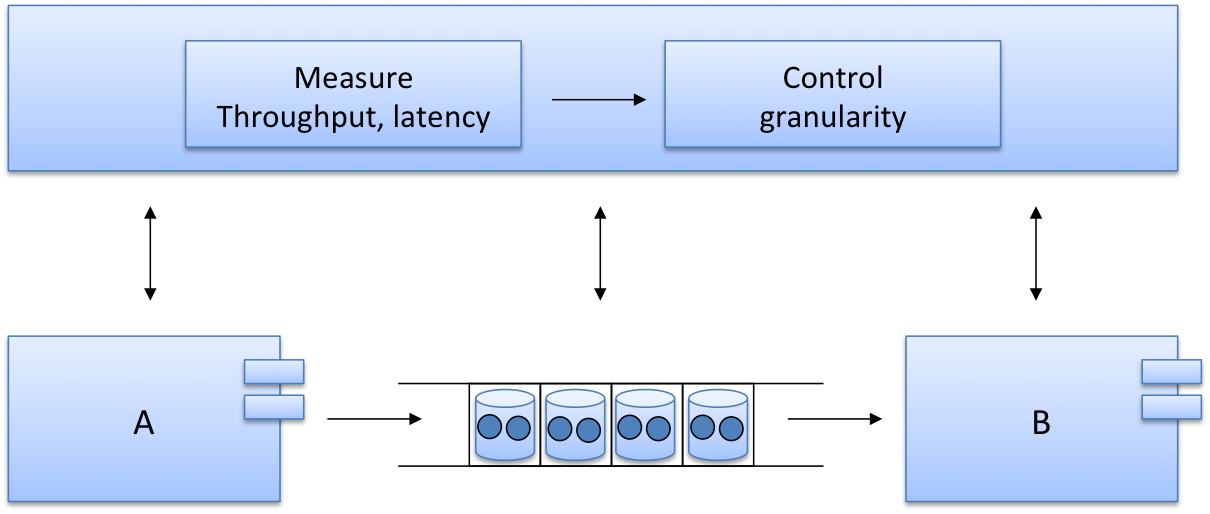
\includegraphics[width=\columnwidth]{ch5_monitoring_control}
	\caption{Monitoring and Control}
	\label{fig:ch05_monitoring_control}
\end{figure}

Aggregation size is not static, depends on the current load of the system:
\begin{itemize}
	\item If the current load of the system is low, aggregation size can be small to provide a low end-to-end latency of the system.
	\item If the current load of the system is high, aggregation size should be high to provide a high maximum throughput of the system. 
\end{itemize}

Monitoring component continuously monitors the the load of the system. 

To control the level of message aggregation at runtime, the adaptive middleware uses a closed feedback loop as shown in Figure \ref{fig:feedback_loop}.

\begin{itemize}
	\item Control Engineering Methodologies have been identified as a promising solution to implement self-adaptive software systems \citep{Patikirikorala:2012ky}, especially for performance control \citep{Abdelzaher:2003ea}.
	\item In particular, feedback loops provide generic mechanisms for self-adaption \citep{Brun:2009ww}. 
	\item Control engineering is based on control theory, which provides a systematic approach to designing closed loop systems that are stable, accurate, have short settling times, and do not overshoot \citep{Abdelzaher:2008ub}.
\end{itemize}

The feedback loop used by the adaptive middleware has the following properties:

\begin{itemize}
	\item \textbf{Input (u):} Current aggregation size
	\item \textbf{Output (y):} Change of queue size measured between sampling intervals
	\item \textbf{Set point (r):} The change of queue size should be zero.
\end{itemize}

Ultimately, we want to control the average end-to-end latency depending on the current load of the system. The change of queue size seems to be an appropriate quantity because it can be directly measured without a lag at each sampling interval, unlike for example the average end-to-end latency.

\begin{figure}[htbp]
	\centering
	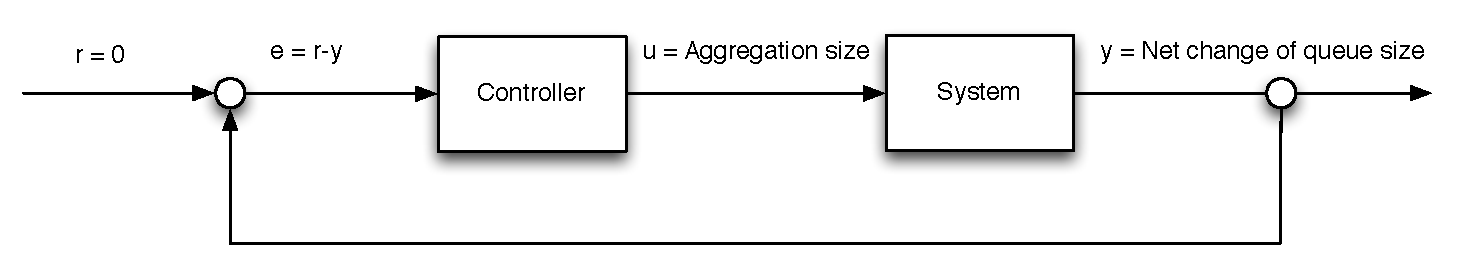
\includegraphics[width=\columnwidth]{feedback_loop}
	\caption{Feedback loop to control the aggregation size}
	\label{fig:feedback_loop}
\end{figure}

\section{Middleware Components}
\label{sec:ch05_middleware_components}
Table \ref{table:ch4_middleware_components} shows the components of the middleware, that are based on the Enterprise Integration Patterns described by \cite{Hohpe:2003fk}.

\begin{table}[htpb]
	\caption{Components of the Adaptive Middleware. We are using the notation defined by \cite{Hohpe:2003fk}}
	\label{table:ch4_middleware_components}
	\centering
	\begin{tabular}{|m{3cm}|m{2cm}|m{5cm}|}
		\hline
		\bfseries Symbol & \bfseries Component & \bfseries Description\\
		\hline 
		\begin{center}
			
\includegraphics[scale=0.5]{message_symbol}
		\end{center} 
		& Message & A single message representing a business event.\\
		\hline 
		\begin{center}
			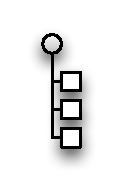
\includegraphics[scale=0.5]{aggregate_symbol} 
		\end{center}
		& Message Aggregate & A set of messages aggregated by the Aggregator component.\\
		\hline
		\begin{center}
			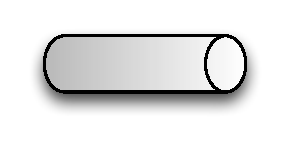
\includegraphics[scale=0.5]{queue_symbol} 
		\end{center}
		& Queue & Storage component which stores messages using the \ac{FIFO} principle.\\
		\hline 
		\begin{center}
			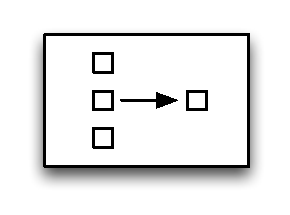
\includegraphics[scale=0.5]{aggregator_symbol}
		\end{center}
		& Aggregator & Stateful filter which stores correlated messages until a set of messages is complete and sends this set to the next processing stage in the messaging route.\\
		\hline
		\begin{center}
			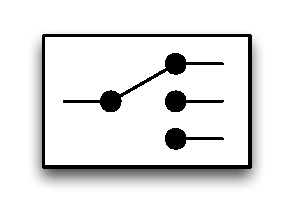
\includegraphics[scale=0.5]{router_symbol} 
		\end{center}
		& Router & Routes messages to the appropriate service endpoint, for example depending on the aggregation size of the message.\\
		\hline
		\begin{center}
			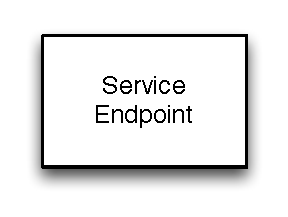
\includegraphics[scale=0.5]{endpoint_symbol} 
		\end{center}
		& Service Endpoint & Represents a business service.\\
		\hline
	\end{tabular}
\end{table}

\section{Design Aspects}
\label{sec:ch05_design_aspects}
This section describes aspects that should be taken into account when designing an adaptive system for bulk data processing.

\subsection{Usage Scenarios}
\todo[inline]{do we need this?}
\begin{landscape}
	\begin{figure*}[htpb]
		\centering
		\mbox{\subfloat[request/response integration pattern]{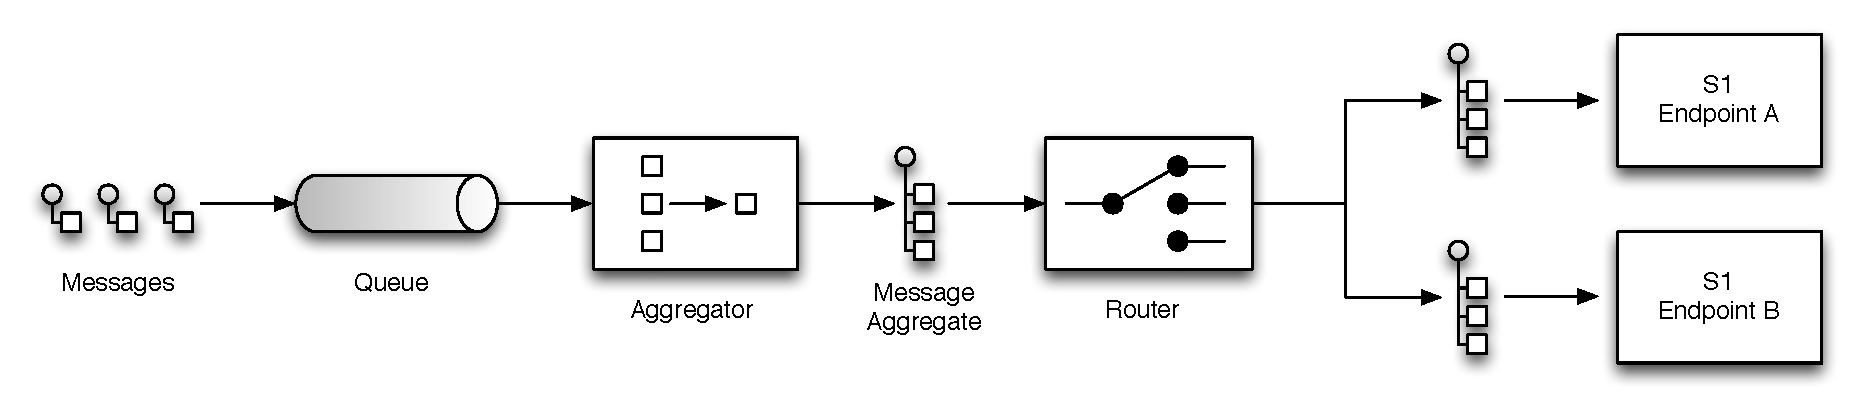
\includegraphics[scale=0.5]{ch5_usage_scenario_1}\label{fig:ch4_usage_scenario_1}}}
		\mbox{\subfloat[point-to-point channel integration pattern]{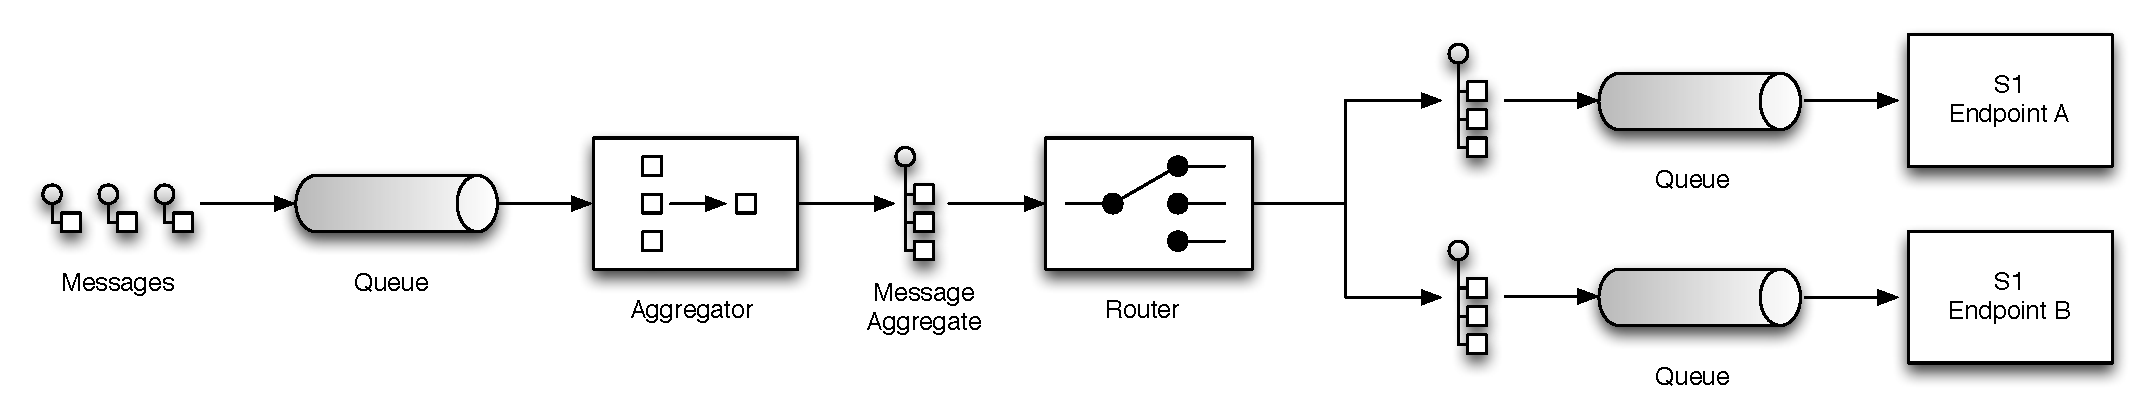
\includegraphics[scale=0.5]{middleware_components}}}
		\caption{Usage scenarios}
	\end{figure*}
\end{landscape}

\begin{itemize}
	\item different usage scenarios
	\item single aggregator, request/response integration pattern
	\item single aggregator, point to point channel
	\item system consisting of multiple subsystems, with each subsystem having an input queue, aggregator, router
\end{itemize}

\subsection{Service Design}
\label{sec:ch05_service_design}

The services that implement the business functionality of the system need to be explicitely designed to support the runt-time adaption between single-event and batch processing. 

There are different options for the design of these services:
\begin{itemize}
	\item Single Service interface with distinct operations for single and batch processing
	\begin{itemize}
		\item The service provides different distinct operations for high and low aggregation sizes with optimized implementations for batch and single-event processing. The decision which operation should be called is done by the message router. It is generally not possible to use different transports for different aggregation sizes.
	\end{itemize}
	\item Single Service interface with a single operation for both single and batch processing
	\begin{itemize}
		\item The service provides a single operation that is called for all aggregation sizes. The decision which optimization should be used is done by the service implementation. It is not possible to use different transports for different aggregation sizes.
	\end{itemize}
	\item Multiple service interfaces for single and batch processing (or different aggregation sizes)
	\begin{itemize}
		\item The logical business service is described by distinct service interfaces which contain operations for either batch processing or single-event processing. The decision which operation should be called is done by the message router. It is possible to use different transports for different aggregation sizes.
	\end{itemize}
\end{itemize}

The choice of service design relates to where you want to have the logic for the message routing for optimized processing. With a single service offering distinct operations for single-event and batch processing, as well as with distinct service for each processing style, the message router decides which service endpoint should be called. In contrast, using a single service with a single operation for both processing styles, the service itself is responsible for choosing the appropriate processing strategy. Using a different integration type for each processing style is not possible in this case.

Table \ref{table:ch05_service_design} shows the advantages and disadvantages for each service design option.

Listing \ref{listing:ch5_service_design_if} shows the interface of a service offering different operations for batch processing (line 6) and single-event processing (line 10).

\begin{lstlisting}[caption={Java interface of a web  service offering different operations for single and batch processing.},label=listing:ch5_service_design_if]
	@WebService
	@SOAPBinding(style=Style.DOCUMENT, use=Use.LITERAL, parameterStyle=ParameterStyle.WRAPPED)
	public interface RatingPortType {
		@WebMethod(operationName="processCallDetails")
		@WebResult(name="costedEvents")
		public Costedevents processCallDetails(@WebParam(name="callDetailRecords") SimpleCDRs callDetailRecords) throws ProcessingException, Exception;
	
		@WebMethod(operationName="processCallDetail")
		@WebResult(name="costedEvent")
		public Costedevent processCallDetail(@WebParam(name="simpleCDR") SimpleCDR callDetailRecord) throws ProcessingException, Exception;
	}
\end{lstlisting}

\begin{table}[htpb]
	\centering
	\begin{tabularx}{\textwidth}{@{} X X X @{}}
		\caption{Options for designing service interfaces}\label{table:ch05_service_design}\\
		\toprule
		\bfseries Interface option & \bfseries Pros & \bfseries Cons\\
		\midrule
		Single service /\\distinct Operations & \savespace
		\begin{titemize}
			\item Lorem ipsum
		\end{titemize} & \savespace
		\begin{titemize}
			\item Lorem ipsum
		\end{titemize}\\
		\midrule
		Single service /\\single operation & \savespace
		\begin{titemize}
			\item 
		\end{titemize} & \savespace
		\begin{titemize}
			\item Lorem ipsum
		\end{titemize}\\
		\midrule
		Distinct services & \savespace
		\begin{titemize}
			\item
		\end{titemize} & \savespace
		\begin{titemize}
			\item Lorem ipsum
		\end{titemize}\\
		\bottomrule
	\end{tabularx}
\end{table}

\subsection{Integration and Transports}
\label{sec:ch05_transports}
The integration architecture defines the technologies that are used to integrate the business services. In general, different integration styles with different transports are used for batch processing and single-event processing, which needs to be taken into account when designing an adaptive system for bulk data processing (Please refer to Section \ref{sec:batch_processing} and \ref{sec:message_processing} for a detailed description of each processing style).

When using high aggegration sizes, it is not feasible to use the same transports as with low aggregation sizes. Large messages should not be transferred over the messaging system. Instead, a file based transport using \ac{FTP} or database-based integration should be used. When using a messaging system, the payload of large messages should not be transported over the messaging system. For example by implementing the \emph{Claim Check} \ac{EIP} (refer to Section \ref{sec:ch03_eip} for a detailed description of this pattern). Table \ref{table:ch05_transports} summarizes the transport options for low and high aggregation sizes.

\begin{table}[htbp]
	\centering
	\begin{tabularx}{\textwidth}{@{} X X X @{}}
		\caption{Transport options for high and low aggregation sizes}\label{table:ch05_transports}\\
		\toprule
		\bfseries Aggregation Size & \bfseries Transport Options\\
		\midrule
		High & \savespace
		\begin{titemize}
			\item Database
			\item File-based (e.g. \ac{FTP})
			\item Claim Check \ac{EIP}
		\end{titemize}\\
		\midrule
		Low & \savespace
		\begin{titemize}
			\item \ac{JMS}
			\item SOAP
		\end{titemize}\\
		\bottomrule
	\end{tabularx}
\end{table}

Additionally, the technical data format should be considered. 

The concrete threshold between low and high aggregation sizes depends on the integration architecture and implementation of the system, such as the integration architecture and the deployed messaging system.

The choice of the appropriate integration transport for a service is implicitly implemented by the message router (see Section \ref{sec:ch05_router}).

\subsection{Error Handling}

Message aggregation has also an impact on the handling of errors that occur during the processing. Depending on the cause of the error, there are two common types of errors: 
\begin{itemize}
	\item \textbf{Technical errors}\\
	Technical errors are errors caused by technical reasons, for example an external system is not availaible or does not respond within a certain timeout or the processed message has an invalid format.
	\item \textbf{Business errors}\\
	Business errors are caused by violation of business rules, for example a call detail record contains a tariff that is no longer valid.
\end{itemize}

The following points should be taken into account, when designing the error handling for an adaptive system for bulk data processing:
\begin{itemize}
	\item Write erroneous messages to an error queue for later processing. 
	\item Use multiple queues for different types of errors, for example distinct queues for technical and business errors to allow different strategies for handling them. Some type of errors can be fixed automatically, for example an error that is caused by an outage of an external system, while other errors need to be fixed manually.
	\item If the erroneous messages is part of an aggregated message, it should be extracted from the aggregate to prevent the whole aggregate from beeing written to the error qeue, especially when using high aggregation sizes.
\end{itemize}

\subsection{Controller Design}
\label{sec:ch05_controller_design}

There are several approaches for the implementation of feedback-control system. \cite{Hellerstein:2004a} describe two major steps:
\begin{enumerate}
	\item modeling the dynamics of the system
	\item developing a control system
\end{enumerate}

There are different approaches that are used in practice to model the dynamics of a system \citep{Hellerstein:2004tu}:
\begin{itemize}
	\item Empirical approach
	\item Black-box modeling
	\item Modeling using stochastic approaches, especially queuing theory
	\item Modeling using special purpose representations, for example the first principles analysis
\end{itemize}

The following approach has been taken in this research:
\begin{enumerate}
	\item Define the control problem
	\item Define the input and output variables of the system
	\item Measure the dynamics of the system
	\item Create a model of the system
	\item Develop the control system
\end{enumerate}

\subsubsection{Control Problem}

\begin{itemize}
	\item Control problem: minimise the end-to-end latency of the system by controlling the message aggregation size
	\item aggregation size used by the messaging system should depend on the current load of the system
	\item when system faces high load, aggregation sizes should be increased
	\item when sytem faces low load, aggregation sizes could be decreases
\end{itemize}
\subsubsection{Input/Output Variables}

\begin{itemize}
	\item \textbf{Input (u):} Current aggregation size
	\item \textbf{Output (y):} Change of queue size measured between sampling intervals
	\item \textbf{Set point (r):} The change of queue size should be zero.
	\item advantage of queue size as output variable: queue size can be directly measured whithout a delay
\end{itemize}

\subsubsection{Control Strategy}

\paragraph{Simple controller}\mbox{}\\
A simple control strategy could be implemented as follows:
\begin{itemize}
	\item change queue > 0: Increase the aggregation size by a certain amount
	\item change queue = 0: Do nothing
\end{itemize}

\paragraph{PID controller}\mbox{}\\
Another option would be to use a standard PID-Controller instead, which calculates the output value $u_k$ at time step $k$ of the controller depending on the current (proportional part), previous (integral part) and expected future error (differential part):
\begin{displaymath}
	u_k=K_p*e_k+K_i*T_a\sum_{i=0}^k e_i+\frac{K_d}{T_a}(e_k-e_{k-1})
\end{displaymath}
with $K_p$ being the controller gain of the proportional part, $e_k$ being the error ($r-y$) at step $k$, $K_i$ being the controller gain of the integral part, $T_a$ being the sampling interval and $K_d$ being the controller gain of the differential part.

\section{Prototype Implementation}
\label{sec:ch05_prototype}

This section describes the implementation of the prototype which implements the core concepts of the adaptive middleware. The prototype is based on the messaging prototype described in Section \ref{sec:ch04_messaging_prototype}.

\todo[inline]{Insert image from section \ref{sec:ch04_messaging_prototype}}

\subsection{Aggregator}

\begin{itemize}
	\item Implementation is based on the aggregator of the messaging prototype as described in Section \ref{sec:ch4_impact_granularity}
\end{itemize}

\begin{lstlisting}[caption={UsageEventsAggrationStrategy},label=listing:ch5_UsageEventsAggrationStrategy]
public class UsageEventsAggrationStrategy implements AggregationStrategy {

	@Override
	public Exchange aggregate(Exchange oldExchange, Exchange newExchange) {
		if (oldExchange == null) {
			RawUsageEvent rawUsageEvent = newExchange.getIn().getBody(RawUsageEvent.class);
			RawUsageEvents rawUsageEvents = new RawUsageEvents();
			List<RawUsageEvent> usageEventList = new ArrayList<RawUsageEvent>();
			rawUsageEvents.setUsageEvents(usageEventList);
			usageEventList.add(rawUsageEvent);
			newExchange.getIn().setBody(rawUsageEvents);
			increaseAggregateSize(newExchange);
			
			Long startTime = getStartTime(newExchange);
			addStartTime(newExchange, startTime);
			
			return newExchange;
		}
		else {
			RawUsageEvents rawUsageEvents = oldExchange.getIn().getBody(RawUsageEvents.class);
			RawUsageEvent rawUsageEvent = newExchange.getIn().getBody(RawUsageEvent.class);
			rawUsageEvents.getUsageEvents().add(rawUsageEvent);
			increaseAggregateSize(oldExchange);
			
			Long startTime = getStartTime(newExchange);
			addStartTime(oldExchange, startTime);
			
			return oldExchange;
		}
	}
	
	//Additional methods removed for simplification...
	
}
\end{lstlisting}

\begin{lstlisting}[caption={Aggregator configuration in definition of BillingRoute},label=listing:ch5_aggregator_definition]
.aggregate(constant(true), new UsageEventsAggrationStrategy())
	.completionSize(header(completionSizeHeader))
	.completionTimeout(completionTimeout)
	.parallelProcessing()
\end{lstlisting}

\subsection{Feedback-Control Loop}

Figure \ref{fig:ch05_components_feedback_loop} shows the components of the feedback-control loop.

\begin{figure}[htbp]
	\centering
	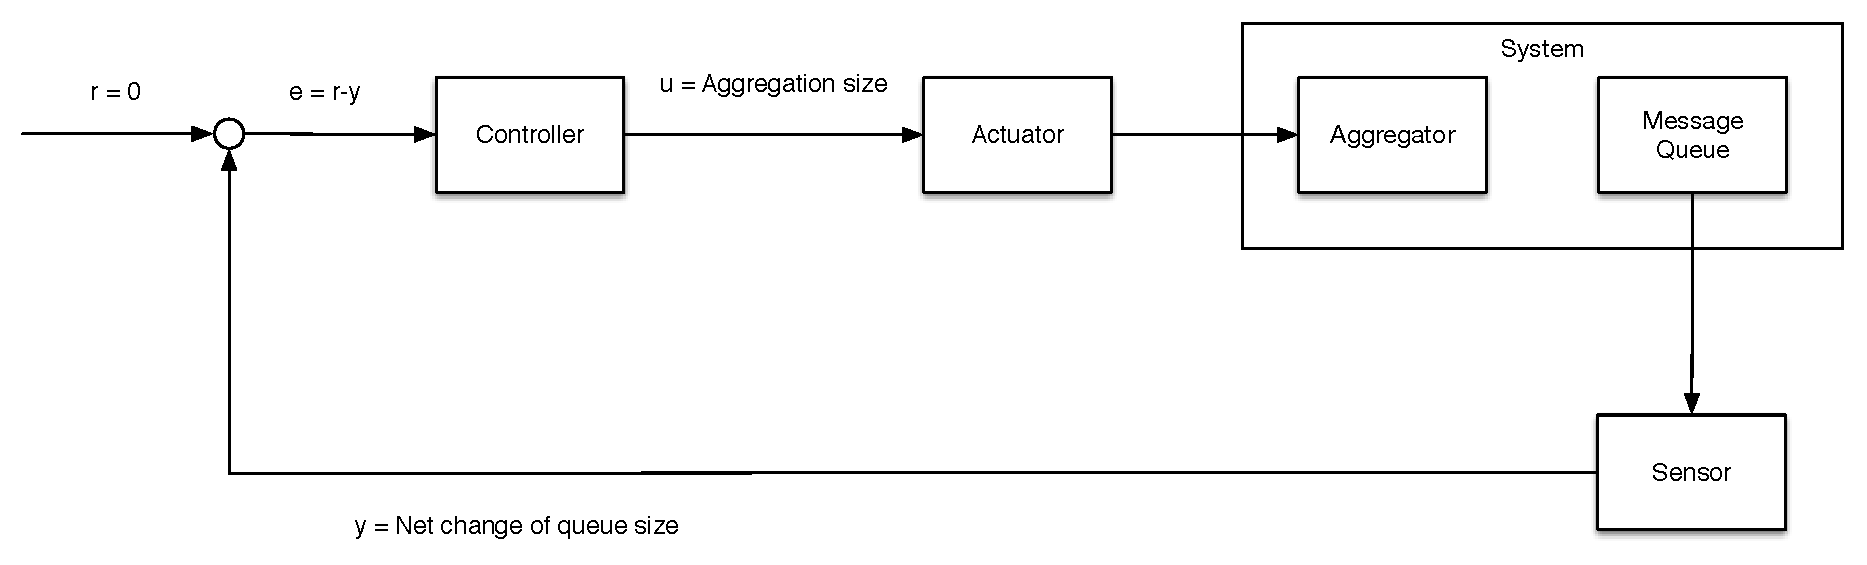
\includegraphics[width=\columnwidth]{ch05_components_feedback-loop}
	\caption{Components of the feedback-control loop}
	\label{fig:ch05_components_feedback_loop}
\end{figure}

\subsubsection{Sensor}

\begin{itemize}
	\item Base class JmxSensor
	\item Reads the current queue length of the ActiveMQ instance using JMX
\end{itemize}

\subsubsection{Controller}

\begin{itemize}
	\item ControllerStrategy Interface
\end{itemize}

\begin{lstlisting}[caption={ControllerStrategy Interface},label=listing:ch5_controller_strategy]
package com.jswiente.phd.performance.controller;

public interface ControllerStrategy {
	public Double getOutput(Double error);
}
\end{lstlisting}

\paragraph{Simple Controller}\mbox{}\\

\paragraph{PID Controller}\mbox{}\\

\begin{lstlisting}[caption={Implementation of PID Controller},label=listing:ch5_pid_controller]
public class PIDController implements ControllerStrategy {
	
	@Value("${controller.kp}")
	private Double kp;
	
	@Value("${controller.ki}")
	private Double ki;
	
	@Value("${controller.kd}")
	private Double kd;
	
	@Value("${controller.ta}")
	private Double ta;
	
	private Double errorSum = 0.0;
	private Double previousError = 0.0;

	public Double getOutput(Double error) {
		errorSum = errorSum + error;
		Double output = kp * error + ki * ta * errorSum + (kd * (error - previousError)/ta);
		previousError = error;
		return output;
	}

	//Setter methods removed for simplification...

}

\end{lstlisting}

\subsubsection{Actuator}

\begin{itemize}
	\item Interface Actuator
	\item AggregateSizeActuator
	\begin{itemize}
		\item Implements Actuator interface
		\item Sets the completionSize of the Aggregator by setting a specific header in the currently processed exchange
	\end{itemize}
\end{itemize}
\begin{lstlisting}[caption={Actuator Interface},label=listing:ch5_actuator_interface]
package com.jswiente.phd.performance.actuator;

public interface Actuator<T> {

	public void setValue(T value);
}
\end{lstlisting}

\begin{lstlisting}[caption={AggregateSizeActuator},label=listing:ch5_aggregateSizeActuator]
@Component
public class AggregateSizeActuator implements Processor, Actuator<Double> {

	@Value("${camel.aggregator.completionSize}")
	private long aggregateSize;
	
	@Value("${camel.aggregator.completionSizeHeader}")
	private String completionSizeHeader;
	
	private static final Logger logger = LoggerFactory
			.getLogger(AggregateSizeActuator.class);
	
	@Override
	public void process(Exchange exchange) throws Exception {
		exchange.getIn().setHeader(completionSizeHeader, aggregateSize);
	}

	@ManagedAttribute
	public long getAggregateSize() {
		return aggregateSize;
	}

	@ManagedAttribute
	public void setAggregateSize(long aggregateSize) {
		logger.debug("Setting aggregateSize to: " + aggregateSize);
		this.aggregateSize = aggregateSize;
	}

	@Override
	public void setValue(Double value) {
		logger.debug("Actuator: Setting aggregateSize to: " + value);
		long aggregateSize = Math.round(value);
		this.setAggregateSize(aggregateSize);
	}

}

\end{lstlisting}

\subsection{Load Generator}

The \emph{Load Generator} is used to generate the system load by generating events (\acp{CDR}) and writing them to the the message queue of the system. It is implemented as a stand-alone Java program using a command-line interface.

\subsubsection{Overview}

Figure \ref{fig:ch5_datagenerator_classdiagram} shows the \ac{UML} class diagram of the load generator.

\begin{figure}[htpb]
	\centering
	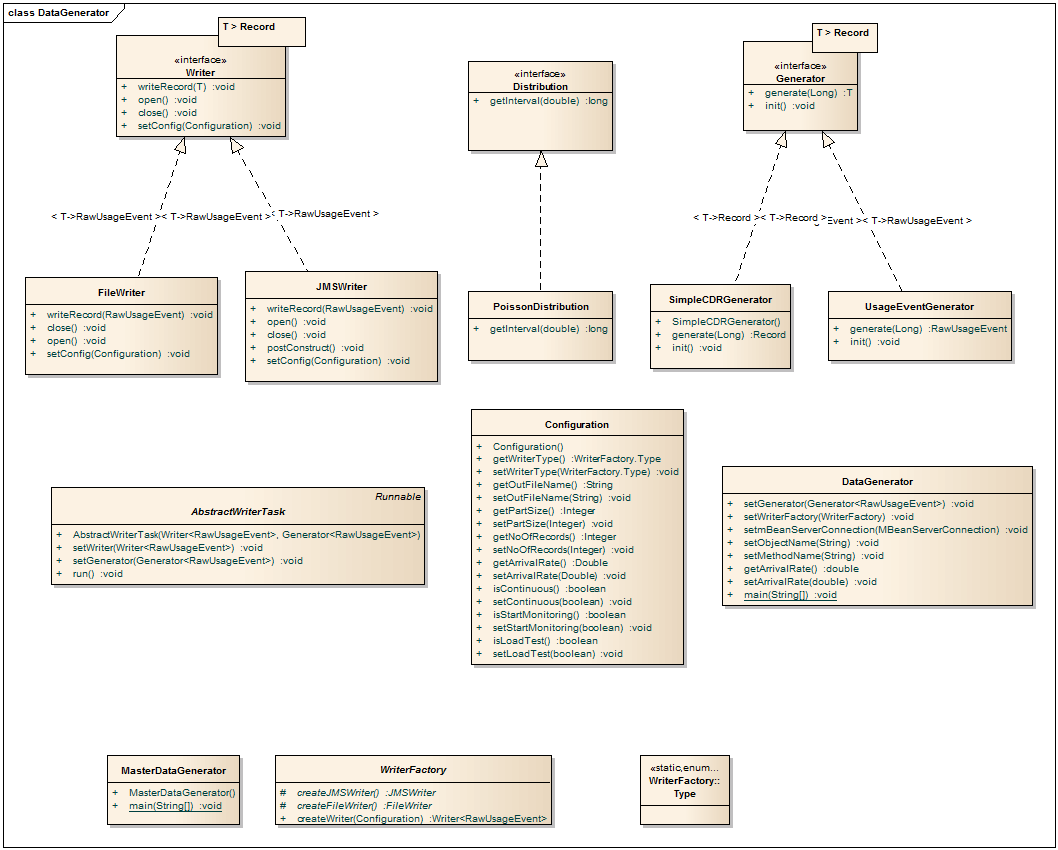
\includegraphics[width=\textwidth]{ch6_datagenerator_classdiagram}
	\caption{\ac{UML} class diagram of the \emph{Load Generator}}
	\label{fig:ch5_datagenerator_classdiagram}
\end{figure}

\begin{itemize}
	\item Description of main classes
\end{itemize}

\subsubsection{Event Distribution}

\begin{itemize}
	\item Poisson Process
	\begin{itemize}
		\item Events occur continuously and independently of each other
		\item Exponentially distributed inter-arrival times
	\end{itemize}
\end{itemize}

\section{Evaluation}
\label{sec:ch05_evaluation}

The prototype described in the previous section has been used to evaluate the concepts of adaptive middleware. 

\begin{itemize}
	\item Goals of the evaluation
\end{itemize}

\subsection{Test Environment}

\begin{itemize}
	\item Same test environment has been used as described in Section \ref{sec:ch4_test_environment}
\end{itemize}

\subsection{Test Design}

\cite{Abdelzaher:2008ub} define a set of properties, that should be considered when designing feedback-control systems for computing systems, called the \acsu{SASO} properties (\textbf{S}table, \textbf{A}ccurate, \textbf{S}ettling times, \textbf{O}vershoot):

\begin{itemize}
	\item \textbf{Stability}
	\item \textbf{Accuracy}
	\item \textbf{Settling time}
	\item \textbf{Overshoot}
\end{itemize}

\subsubsection{Static Tests}
\label{sec:ch05_static_tests}

\subsubsection{Step Tests}
\label{sec:ch05_step_tests}

\subsubsection{Dynamic Tests}

\begin{itemize}
	\item Definition of test cases
\end{itemize}

\subsection{Results}

\section{Discussion with respect to related work}\label{sec:ch5_related_work}
\subsection{Adaptive Middleware}
Research on messaging middleware currently focusses on Enterprise Services Bus (ESB) infrastructure. An ESB is an integration plattform that combines messaging, web services, data transformation and intelligent routing to connect multiple heterogeneous services \citep{Chappell:2004jo}. It is a common middleware to implement the integration layer of an Service Oriented Architecture (SOA) and is available in numerous commercial and open-source packages.

Several research has been done to extend the static service composition and routing features of standard ESB implementations with dynamic capabilities decided at run-time, such as dynamic service composition \citep{Chang:2007aa}, routing \citep{Bai:2007aa} \citep{Wu:2008aa} \citep{Ziyaeva:2008aa} and load balancing \citep{Jongtaveesataporn:2010aa}.

Work to manage and improve the Quality of Service (QoS) of ESB and service-based systems in general is mainly focussed on dynamic service composition and service selection based on monitored QoS metrics such as throughput, availability and response time \citep{Calinescu:2011aa}. \cite{Gonzalez:2011} propose an adaptive ESB infrastructure to adress QoS issues in service-based systems which provides adaption strategies for response time degradation and service saturation, such as invoking an equivalent service, using previously stored information, distributing requests to equivalent services, load balancing and deferring service requests.

\subsection{Message Batching}
The adaption strategy of our middleware is to change the message aggregation size based on the current load of the system. Aggregating or batching of messages is a common approach to increase the throughput of a messaging system, for example to increase the throughput of total ordering protocols \citep{Friedman:1997aa} \citep{Friedman:2006aa} \citep{Romano:2012aa} \citep{Didona:2012aa}.


\subsection{Dynamic Scaling}
A different solution to handle infrequent load spikes is to automatically instantiate additional server instances, as provided by current Platform as a Service (PaaS) offerings such as Amazon EC2 \citep{ec2_autoscaling} or Google App Engine \citep{google_cloud_autoscaling}. While scaling is a common approach to improve the performance of a system, it also leads to additional operational and possible license costs. Of course, our solution can be combined with these auto-scaling approaches.

\subsection{Feedback Control of Computing Systems}

\begin{itemize}
	\item General definition of Feedback Control
	\item Properties of Feedback Control Systems
	\item Open-Loop and Closed-Loop Control Systems
	\item Applications for Feedback Control
	\begin{itemize}
		\item Feedback-Control of Software Performance and \ac{QoS} 
	\end{itemize}
\end{itemize}

\begin{itemize}
	\item Feedback Control of Computing Systems \citep{Hellerstein:2004a}
	\begin{itemize}
		\item Applications of Control Theory to Computing Systems
		\item Examples of Feedback Control Systems
	\end{itemize}
	\item Introduction to Control Theory And Its Application to Computing Systems \citep{Abdelzaher:2008ub}
	\item Challenges of Feedback Control of Computing Systems \citep{Hellerstein:2004tu}
	\item A Systematic Survey on the Design of Self-Adaptive Software Systems using Control Engineering Approaches \citep{Patikirikorala:2012ky}
	\item Control Systems application in Java based Enterprise and Cloud Environments \- A Survey \citep{Gullapalli:2011vn}
	\item Engineering Self-Adaptive Systems through Feedback Loops \citep{Brun:2009ww}
\end{itemize}

\begin{itemize}
	\item Feedback-Control of Software Performance and \ac{QoS}
	\begin{itemize}
		\item Feedback Performance Control in Software Services \citep{Abdelzaher:2003ea}
		\item ControlWare: A Middleware Architecture for Feedback Control of Software Performance \citep{Zhang:2002gf}
		\item Intelligent Enterprise Application Servers: A Vision for Self-Managing Performance \citep{Kumar:2013bw}
		\item Throughput Improvement in Distributed Systems - An Investigation on Java Messaging Servers using Adaptive Control
		\item Self-regulating Message Throughput in Enterprise Messaging Servers - A Feedback Control Solution \citep{Kumar:2012we}
	\end{itemize}
\end{itemize}

\section{Summary}\label{sec:ch5_summary}
In this paper, we have presented a middleware that is able to adapt itself to changing load scenarios by fluently shifting the processing type between single event and batch processing. The middleware uses a closed feedback loop to control the end-to-end latency of the system by adjusting the level of message aggregation depending on the current load of the system. Determined by the aggregation size of a messsage, the middleware routes a message to appropriate service endpoints, which are optimized for either single-event or batch processing.

To evaluate the proposed middleware concepts, we have implemented a prototype system and performed preliminary performance tests. The tests show that throughput and latency of a messaging system depend on the level of data granularity and that the throughput can be increased by increasing the granularity of the processed messages.

Next steps of our research are the implementation of the proposed middleware including the evaluation and tuning of different controller architectures, performance evaluation of the proposed middleware using the prototype and developing a conceptional framework containing guidelines and rules for the practitioner how to implement an enterprise system based on the adaptive middleware for near-time processing

\cleardoublepage

%!TEX root = ../thesis.tex
%******************************************************************************
\chapter[Conceptual Framework]{A Conceptual Framework for Feedback-Controlled Bulk Data Processing Systems}\label{ch:conceptual_framework}

%******************************************************************************

\section{Introduction} 

\begin{itemize}
	\item The concept for an adaptive Middleware for bulk data processing presented in chapter \ref{ch:adaptive_middleware} describes the ``What'' (what needs to be done) but not the ``How'' (how should it be done).
	\item The design, implementation and operation of such a system differs from common approaches to implement enterprise systems (what are these differences?)
	\begin{itemize}
		\item Design: Defining Service interfaces, defining aggregation rules, defining transports, defining integration architecture
		\item Implementation: Service implementation, Service Optimisation
		\item Operation: controller tuning, monitoring
	\end{itemize}
	\item In order to guide the implementation of an adaptive system for bulk data processing, a conceptual framework is needed
	\item It defines views, roles and tasks and their dependencies to describe the necessary steps for design, implementation and operation of system describe in Chapter \ref{ch:adaptive_middleware}.
	\item The conceptual model can be tailored to specific projects requirements, it does not have to be followed strictly.
\end{itemize}

\begin{figure}
	[htpb] \centering 
	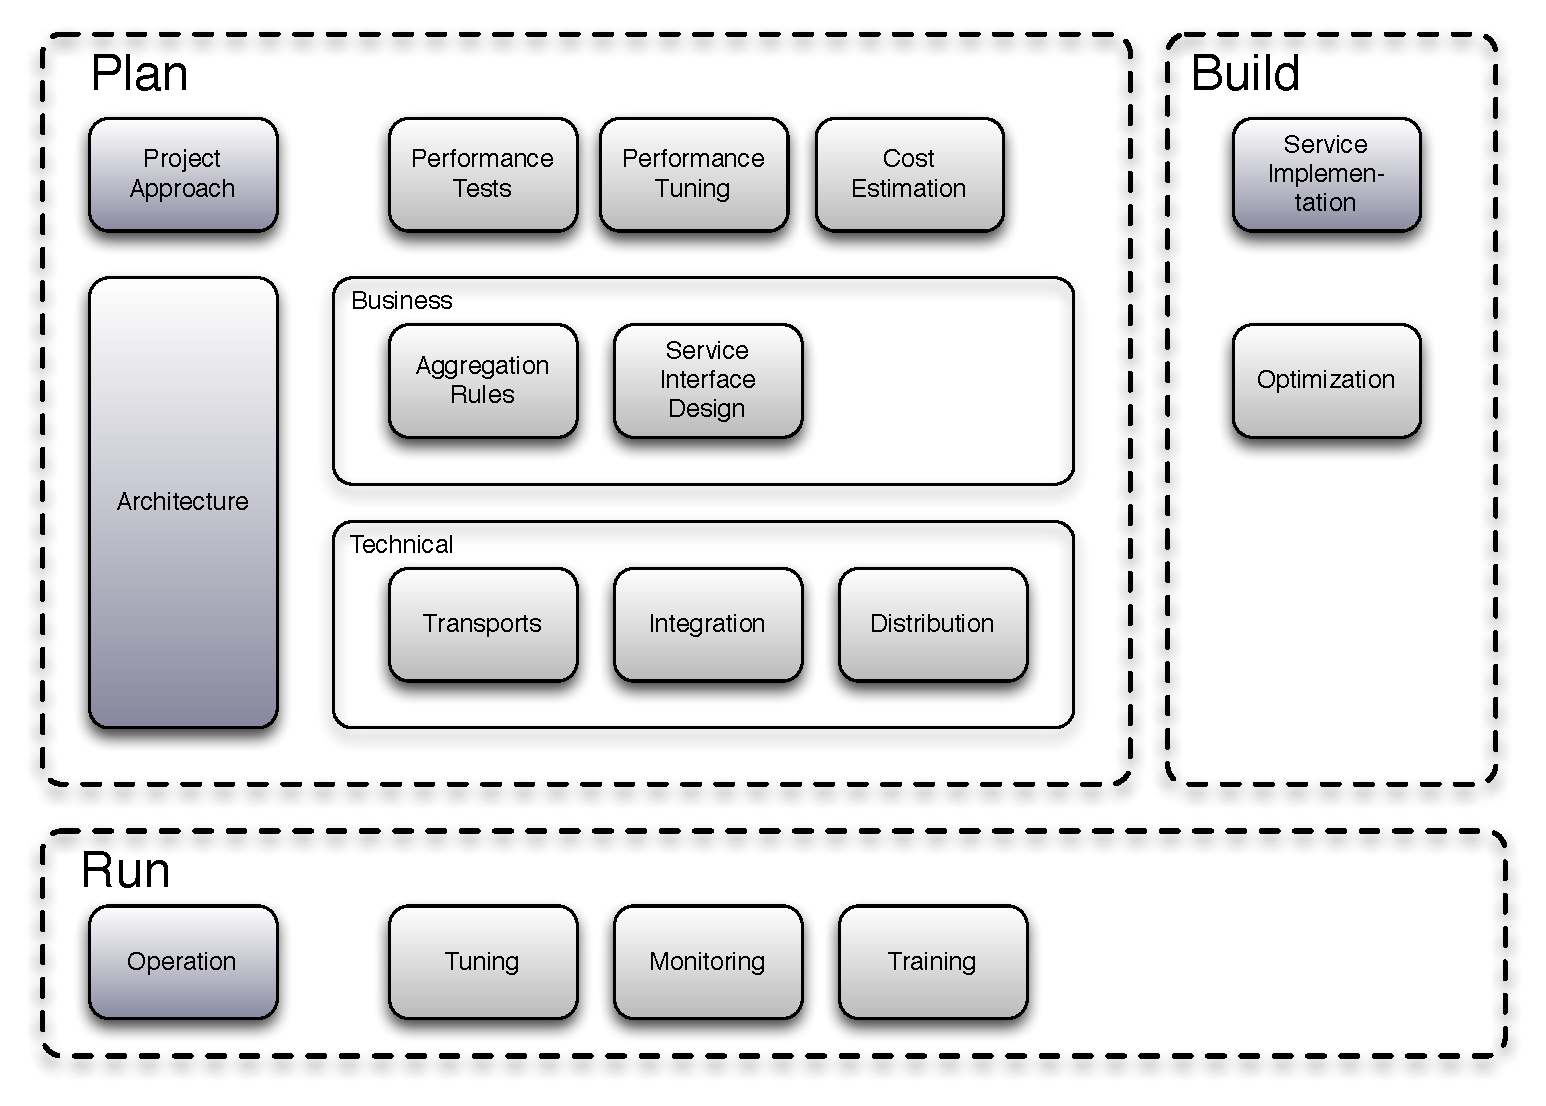
\includegraphics[width=\textwidth]{ch6_conceptual_framework_overview} \caption{Overview of Conceptual Framework} \label{fig:ch6_conceptional_framework_overview} 
\end{figure}

\section{Metamodel} 
The conceptual framework consists of the following entities:
\begin{itemize}
	\item View
	\begin{itemize}
		\item contains Tasks
	\end{itemize}
	\item Role
	\begin{itemize}
		\item processes Tasks
	\end{itemize}
	\item Task
	\begin{itemize}
		\item is contained in a View
		\item is processed by a Role
		\item produces Artifacts
		\item uses Tools
	\end{itemize}
	\item Deliverable
	\begin{itemize}
		\item is produced by a Task
	\end{itemize}
	\item Tool
	\begin{itemize}
		\item is used by a Task
	\end{itemize}
\end{itemize}

\begin{figure}
	[htpb] \centering 
	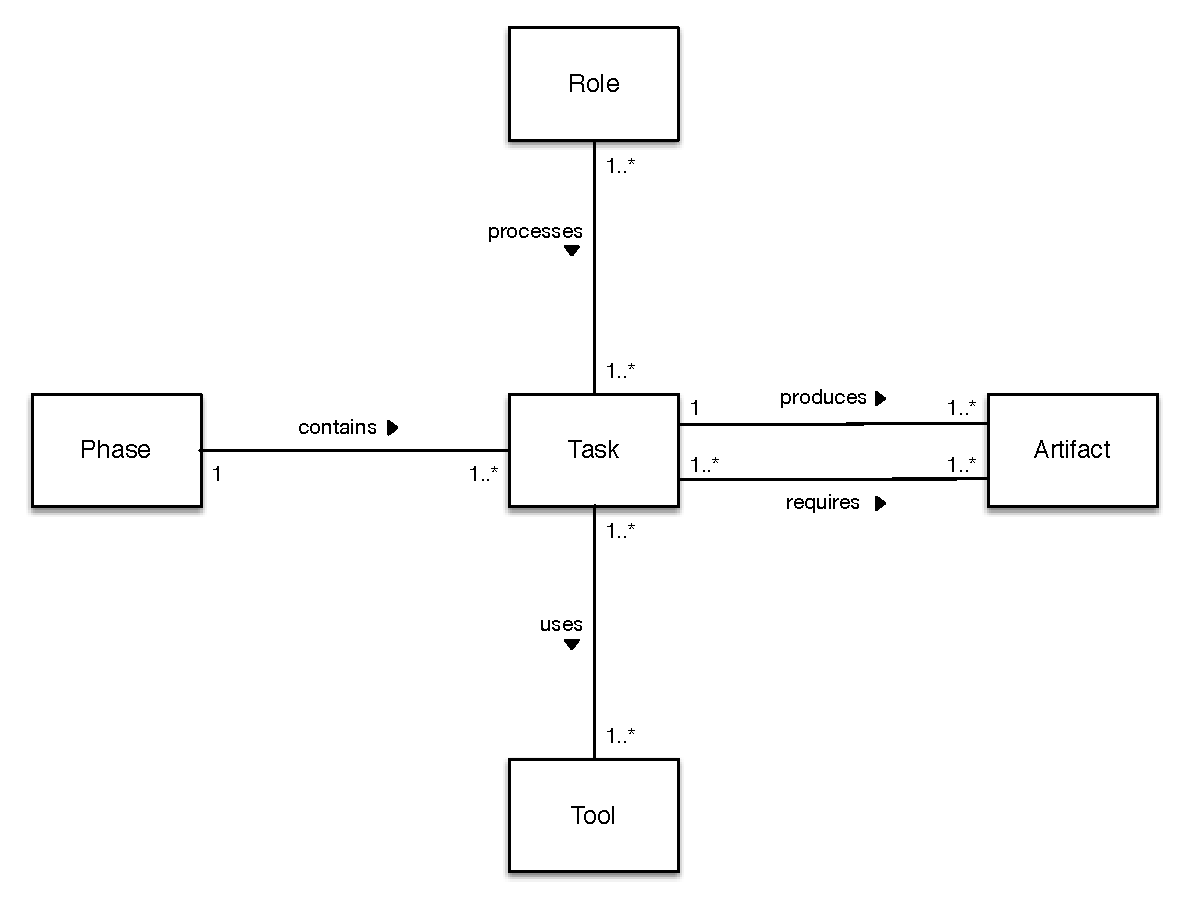
\includegraphics[width=\textwidth]{ch6_metamodel} 
	\caption{Metamodel} 
	\label{fig:ch6_metamodel} 
\end{figure}

\section{Phase}

\begin{itemize}
	\item Phases are the toplevel building blocks
	\item The framework defines the following phases
	\begin{itemize}
		\item Plan
		\item Build
		\item Run
	\end{itemize}
	\item Phases are aligned to phases commonly used by other software development frameworks and methodologies (examples?)
	\item It should be noted that the framework defines no requirements regarding the general order or mode in which theses phases should be processed. It is therefore possible to use this framework with different software development methodologies such as the Waterfall model, Scrum or the V-Modell.
\end{itemize}

\subsection{Plan}
\begin{minipage}{\textwidth}
	\captionof{table}{Phase: Plan}\label{table:ch6_View_Plan}
	\begin{tabular}
		{|m{2cm}|m{10cm}|} \hline \bfseries Phase & Plan\\
		\hline \bfseries Description & This phase contains tasks concerning the technical and business design of the system.\\
		\hline \bfseries Tasks & 
		\begin{itemize}
			\item Define System Architecture
			\item Define Integration Architecture
			\item Define Controller Architecture
			\item Define Service Interfaces
			\item Define Aggregation Rules
			\item Define Performance Tests
			\item Define Training Concept
		\end{itemize}
		\\
		\hline \bfseries Roles &
		\begin{itemize}
			\item Project Manager
			\item Business Analyst
			\item System Architect
			\item Service Architect
		\end{itemize}
		\\
		\hline 
	\end{tabular}
\end{minipage}

\subsection{Build}
\begin{minipage}{\textwidth}
\captionof{table}{Phase: Build}\label{table:ch6_View_Build}
\begin{tabular}
	{|m{2cm}|m{10cm}|} \hline \bfseries Phase & Build\\
	\hline \bfseries Description & This phase contains tasks concerning the implementation of the system.\\
	\hline \bfseries Tasks & 
	\begin{itemize}
		\item Implement Controller and Feedback Loop
		\item Implement Services
		\item Implement Aggregation Rules
		\item Perform Controller Tuning
	\end{itemize}
	\\
	\hline \bfseries Roles &
	\begin{itemize}
		\item Developer
		\item Service Developer
		\item System Architect
		\item Tester
	\end{itemize}
	\\
	\hline 
\end{tabular}
\end{minipage}

\subsection{Run}
\begin{minipage}{\textwidth}
\captionof{table}{Phase: Run}\label{table:ch6_View_Run}
\begin{tabular}
	{|m{2cm}|m{10cm}|} \hline \bfseries Phase & Run\\
	\hline \bfseries Description & This phase contains tasks concerning the operation of the implemented system in the production environment. \\
	\hline \bfseries Tasks & 
	\begin{itemize}
		\item Setup Monitoring infrastructure
		\item Setup Test and Integration Environment
		\item Deploy to Test and Integration Environment
		\item Perform Performance Tests
		\item Evaluate Performance Test Results
	\end{itemize}
	\\
	\hline \bfseries Roles &
	\begin{itemize}
		\item Operations Engineer
		\item Systems Architect
		\item Developer
	\end{itemize}
	\\
	\hline 
\end{tabular}
\end{minipage}

\section{View}
\todo[inline]{Do we need Views?}
\begin{itemize}
	\item Technical
	\item Business
\end{itemize}

\section{Roles} 

\begin{itemize}
	\item Roles describe responsibilities and skills
	\item Roles are not the same as persons, a person can fulfill multiple roles at the same time
\end{itemize}

The following Roles are defined:
\begin{itemize}
	\item System Architect 
	\item Business Architect
	\item Developer
	\item Test Engineer
	\item Project Manager
	\item Operations Engineer 
	\item Service Architect 
	\item Service Developer
\end{itemize}

\subsection{System Architect} 
\begin{minipage}{\textwidth}
\captionof{table}{System Architect}\label{table:ch6_Role_System_Architect}
\begin{tabular}
	{|m{2cm}|m{10cm}|} \hline \bfseries Role & System Architect\\
	\hline \bfseries Description & The System Architect is responsible for designing the technical architecture of the system, including the integration and controller architecture.\\
	\hline \bfseries Tasks & 
	\begin{itemize}
		\item Define System Architecture 
		\item Define Integration Architecture
		\item Define Controller Architecture
		\item Define Service Interfaces (?)
	\end{itemize}
	\\
	\hline 
\end{tabular}
\end{minipage}

\subsection{Business Analyst}
\begin{minipage}{\textwidth}
\captionof{table}{Business Architect} \label{table:ch6_Role_Business_Analysist}
\begin{tabular}
	{|m{2cm}|m{10cm}|} \hline \bfseries Role & Business Analyst\\
	\hline \bfseries Description & The Business Architect is responsible for designing the business architecture of the system, including the definition of services and aggregation rules.\\
	\hline \bfseries Tasks & 
	\begin{itemize}
		\item Define Services (?)
		\item Define Aggregation Rules
	\end{itemize}
	\\
	\hline 
\end{tabular}
\end{minipage}

\subsection{Developer}
\begin{minipage}{\textwidth}
\captionof{table}{Developer} \label{table:ch6_Role_Developer}
\begin{tabular}
	{|m{2cm}|m{10cm}|} \hline \bfseries Role & Developer\\
	\hline \bfseries Description & The Developer is responsible for the implementation of the system, including the implementation and tuning of the feeback-controll loop.\\
	\hline \bfseries Tasks & 
	\begin{itemize}
		\item Implement Integration Mechanisms (?)
		\item Implement Aggregation Rules
		\item Implement Controller
		\item Perform Controller Tuning (?)
	\end{itemize}
	\\
	\hline 
\end{tabular}
\end{minipage}

\subsection{Tester}
\begin{minipage}{\textwidth}
\captionof{table}{Tester} \label{table:ch6_Role_Tester}
\begin{tabular}
	{|m{2cm}|m{10cm}|} \hline \bfseries Role & Test Engineer\\
	\hline \bfseries Description & The Tester is responsible for defining and performing the performance tests of the system.\\
	\hline \bfseries Tasks & 
	\begin{itemize}
		\item Define Performance Tests (?)
		\item Perform Performance Tests
	\end{itemize}
	\\
	\hline
\end{tabular}
\end{minipage}

\subsection{Project Manager}
\begin{minipage}{\textwidth}
\captionof{table}{Project Manager} \label{table:ch6_Role_Project_Manager}
\begin{tabular}
	{|m{2cm}|m{10cm}|} \hline \bfseries Role & Project Manager\\
	\hline \bfseries Description & The Project Manager is responsible for the project coordination, including the staffing and planing of the required environments.\\
	\hline \bfseries Tasks & 
	\begin{itemize}
		\item Plan Staffing (?)
		\item Plan Project Environments (Development / Testing / Integration / Production)
	\end{itemize}
	\\
	\hline 	
\end{tabular}
\end{minipage}

\subsection{Operations Engineer}
\begin{minipage}{\textwidth}
\captionof{table}{Operations Engineer} \label{table:ch6_Role_Operations_Engineer}
\begin{tabular}
	{|m{2cm}|m{10cm}|} \hline \bfseries Role & Operations Engineer\\
	\hline \bfseries Description & The Operations Engineer is responsible for operating the system, including setup, deployment and monitoring.\\
	\hline \bfseries Tasks & 
	\begin{itemize}
		\item Setup Monitoring Infrastructure
		\item Setup Test and Integration Environment
		\item Deploy to Test and Integration Environment 
	\end{itemize}
	\\
	\hline 
\end{tabular}
\end{minipage}

\subsection{Service Architect}
\begin{minipage}{\textwidth}
\captionof{table}{Service Architect} \label{table:ch6_Role_Service_Architect}
\begin{tabular}
	{|m{2cm}|m{10cm}|} \hline \bfseries Role & Service Architect\\
	\hline \bfseries Description & The Service Architect is responsible for designing the technical architecture of services.\\
	\hline \bfseries Tasks & 
	\begin{itemize}
		\item Define Service Interfaces
	\end{itemize}
	\\
	\hline 
\end{tabular}
\end{minipage}

\subsection{Service Developer}
\begin{minipage}{\textwidth}
\captionof{table}{Service Developer} \label{table:ch6_Role_Service_Developer}
\begin{tabular}
	{|m{2cm}|m{10cm}|} \hline \bfseries Role & Service Developer\\
	\hline \bfseries Description & The Service Developer is responsible for implementing the services.\\
	\hline \bfseries Tasks & 
	\begin{itemize}
		\item Implement Service Interface
	\end{itemize}
	\\
	\hline 
\end{tabular}
\end{minipage}

\section{Tasks}
\label{sec:ch6_tasks}

\begin{itemize}
	\item Main entities of the conceptual framework, define what should be done.
	\item Tasks depend on each other, some tasks must be processed in a certain order
\end{itemize}

\begin{figure}[htpb] \centering 
	\includegraphics[width=\textwidth]{ch6_dependencies} 
	\caption{Tasks depend on each other} 
	\label{fig:ch6_dependencies} 
\end{figure}

\begin{itemize}
	\item Define Business Architecture
	\begin{itemize}
		\item Define Service Interfaces
		\item Define Aggregation Rules
	\end{itemize}
	\item Define System Architecture 
	\begin{itemize}
		\item Define Integration Architecture
		\begin{itemize}
			\item Transports
			\item Distribution
		\end{itemize}
		\item Define Routing Rules
		\item Define Controller Architecture 
		\begin{itemize}
			\item Define Control Problem 
			\item Define Input/Output Variables 
		\end{itemize}
		\item Define Routing Rules
	\end{itemize}
	\item Implement Controller / Feedback Loop
	\item Perform Controller Tuning 
	\begin{itemize}
		\item System Model/System Identification 
		\item Static Tests
		\item Step Tests
	\end{itemize}
	\item Implement Service Interfaces / Test / Deploy
	\item Implement Aggregation Rules 
	\item Define Performance Tests 
	\item Setup Monitoring infrastructure
	\item Setup Test and Integration Environment
	\item Deploy to Test and Integration Environment
	\item Perform Performance Tests
	\item Evaluate Performance Test Results
	\item Define Training Concept
\end{itemize}

\subsection{Define Business Architecture}

\begin{itemize}
	\item The business architecture defines the business components of the system and their relationships independantly of the technical implementation.
	\item Except from the described subtasks, the task is not specific to the conceptual model.
\end{itemize}

\subsection{Define Service Interfaces}
\begin{minipage}{\textwidth}
\captionof{table}{Define Service Interfaces} \label{table:ch6_Task_Define_Service_Interfaces}
\begin{tabular}
	{|m{3cm}|m{10cm}|} \hline \bfseries What & Define Service Interfaces\\
	\hline \bfseries Why & Lorem ipsum\\
	\hline \bfseries Who & Business Architect\\
	\hline \bfseries Artifacts & Service Interface Definitions\\
	\hline \bfseries Challenges & Lorem Ipsum\\
	\hline 
\end{tabular}
\end{minipage}

\begin{itemize}
	\item Definition of service operations, every service needs operations for single event and batch processing
	\begin{itemize}
		\item Distinct operations for batch and single event processing
		\item common operation for both processing styles (list interface)
	\end{itemize}
	\item Defines functional format of input and output data
	\item Does not include informations about the technical format, such as \ac{XML} or \ac{JSON}, and the integration style, such SOAP or \ac{REST}
\end{itemize}

\subsection{Define Aggregation Rules}
\begin{minipage}{\textwidth}
\captionof{table}{Define Aggregation Rules} \label{table:ch6_Task_Define_Aggregation_Rules}
\begin{tabular}
	{|m{3cm}|m{10cm}|} \hline \bfseries What & Define Aggregation Rules\\
	\hline \bfseries Why & Lorem ipsum\\
	\hline \bfseries Who & Business Architect\\
	\hline \bfseries Artifacts & Aggregation Rules\\
	\hline \bfseries Challenges & Lorem Ipsum\\
	\hline 
\end{tabular}
\end{minipage}

\begin{itemize}
	\item Definition of rules used in the aggregator for correlating events
	\item Different options
	\begin{itemize}
		\item No correlation
		\begin{itemize}
			\item Simple solution
			\item even distribution of events
			\item optimization is not or hardly possible
		\end{itemize}
		\item Business correlation
		\begin{itemize}
			\item analysation of processed data needed
			\item no even distribution of data (depending on correlation rule), leads to uneven distribution of latency
			\item optimization is possible
		\end{itemize}
		\item Technical correlation
		\begin{itemize}
			\item analysation of processed data needed
			\item Rules can be defined after integration architecture
			\item no even distribution of data (depending on correlation rule), leads to uneven distribution of latency
			\item optimization (?)
		\end{itemize}
	\end{itemize}
\end{itemize}

\subsection{Define System Architecture }
\begin{minipage}{\textwidth}
\captionof{table}{Define System Architecture} \label{table:ch6_Task_Define_System_Architecture}
\begin{tabular}
	{|m{3cm}|m{10cm}|} \hline \bfseries What & Define System Architecture
	Subtasks:
	\begin{itemize}
		\item Define Integration Architecture
		\item Define Controller Architecture
	\end{itemize}
	\\
	\hline \bfseries Why & The System Architecture defines the technical architecture of the system.\\
	\hline \bfseries Who & System Architect\\
	\hline \bfseries Input & 
		\begin{itemize}
			\item Business Architecture
			\item Service Interface Definitions
		\end{itemize}
	\\
	\hline \bfseries Output & System Architecture\\
	\hline \bfseries Tools & \ac{UML}\\
	\hline \bfseries Challenges & \\
	\hline 
\end{tabular}
\end{minipage}

\begin{itemize}
	\item Except from the described subtasks, the task is not specific to the conceptual model.
\end{itemize}

\subsection{Define Integration Architecture}
\begin{minipage}{\textwidth}
\captionof{table}{Define Integration Architecture} \label{table:ch6_Task_Define_Integration_Architecture}
\begin{tabular}
	{|m{3cm}|m{10cm}|} \hline \bfseries What & Define Integration Architecture\\
	\hline \bfseries Why & \\
	\hline \bfseries Who & System Architect\\
	\hline \bfseries Input & 
		\begin{itemize}
			\item Business Architecture
			\item Service Interface Definitions
		\end{itemize}
	\\
	\hline \bfseries Output & Integration Architecture\\
	\hline \bfseries Challenges & \\
	\hline 
\end{tabular}
\end{minipage}

\begin{itemize}
	\item Definition of integration architecture
	\begin{itemize}
		\item Sychronous, e.g. webservices
		\item Asynchronous, e.g. message queues
	\end{itemize}
	\item Definition of transports
	\begin{itemize}
		\item JMS
		\item SOAP
		\item REST
		\item FTP
		\item DB
	\end{itemize}
	\item Different transports / integration patterns needed for different aggregation sizes:
	\begin{itemize}
		\item Large messages should not be transferred over the messaging bus
		\item Options for large messages:
		\begin{itemize}
			\item File-based integration and transfer using FTP or database
			\item Message-Slip EIP pattern
		\end{itemize}
	\end{itemize}
\end{itemize}

\subsection{Define Routing Rules}

\begin{minipage}{\textwidth}
\captionof{table}{Define Routing Rules} \label{table:ch6_Task_Define_Routing_Rules}
\begin{tabular}
	{|m{3cm}|m{10cm}|} \hline \bfseries What & Define Routing Rules\\
	\hline \bfseries Why & \\
	\hline \bfseries Who & System Architect\\
	\hline \bfseries Input & 
		\begin{itemize}
			\item Integration Architecture
		\end{itemize}
	\\
	\hline \bfseries Output & Routing Rules Definition\\
	\hline \bfseries Challenges & Finding the data aggregation threshold to route messages to the appropriate service endpoint.\\
	\hline 
\end{tabular}
\end{minipage}

\begin{itemize}
	\item Depending on the size of the aggregated message, the Router routes the message to the appropriate service endpoint, which is either optimized for batch or single event processing.
	\item The routing rules define, which service endpoint should be called for a given aggregation size.
\end{itemize}

\subsection{Define Controller Architecture}
\begin{minipage}{\textwidth}
\captionof{table}{Define Controller Architecture} \label{table:ch6_Task_Define_Controller_Architecture}
\begin{tabular}
	{|m{3cm}|m{10cm}|} \hline \bfseries What & Define Controller Architecture\\
	\hline \bfseries Why & \\
	\hline \bfseries Who & System Architect\\
	\hline \bfseries Input & System Architecture\\
	\hline \bfseries Output & Controller Architecture\\
	\hline \bfseries Artifacts & System Architecture\\
	\hline \bfseries Challenges & \\
	\hline 
\end{tabular}
\end{minipage}

\begin{itemize}
	\item Design of the controller architecture implemented by the system
	\item For example
	\begin{itemize}
		\item PID Controller
		\item Fuzzy Controller
	\end{itemize}
	\item Depends on control problem and system dynamics (linear, non-linear)
\end{itemize}

\subsubsection{Define Control Problem}
\todo[inline]{Do we need this task or is this already fixed with the proposed middleware architecture?}
\begin{minipage}{\textwidth}
\captionof{table}{Define Control Problem} \label{table:ch6_Task_Define_Control_Problem}
\begin{tabular}
	{|m{3cm}|m{10cm}|} \hline \bfseries What & Define System Architecture\\
	\hline \bfseries Why & Lorem ipsum\\
	\hline \bfseries Who & System Architect\\
	\hline \bfseries Artifacts & System Architecture\\
	\hline \bfseries Challenges & Lorem Ipsum\\
	\hline \bfseries Best practises & Lorem ipsum\\
	\hline 
\end{tabular}
\end{minipage}

\subsubsection{Define Input/Output Variables}
\begin{minipage}{\textwidth}
\captionof{table}{Define Input/Output Variables} \label{table:ch6_Task_Define_Controller_Variables}
\begin{tabular}
	{|m{3cm}|m{10cm}|} \hline \bfseries What & Define Input/Output Variables\\
	\hline \bfseries Why & Lorem ipsum\\
	\hline \bfseries Who & System Architect\\
	\hline \bfseries Artifacts & System Architecture\\
	\hline \bfseries Challenges & Lorem Ipsum\\
	\hline \bfseries Best practises & Lorem ipsum\\
	\hline 
\end{tabular}
\end{minipage}

\begin{itemize}
	\item Definition of input and output variables of the controller
	\item for example
	\begin{itemize}
		\item Number of messages in the system
		\item Input queue length
		\item current end-to-end latency
		\item current throughput
	\end{itemize}
	\item selected input variables should be measured easily and directly, without delay such as when calculating averages
\end{itemize}

\subsection{Implement Controller}
\begin{minipage}{\textwidth}
\captionof{table}{Implement Controller / Feedback Loop} \label{table:ch6_Task_Implement_Controller}
\begin{tabular}
	{|m{3cm}|m{10cm}|} \hline \bfseries What & Implement Controller\\
	\hline \bfseries Why & Lorem ipsum\\
	\hline \bfseries Who & System Architect\\
	\hline \bfseries Input & Controller Architecture\\
	\hline \bfseries Artifacts & Controller Implementation\\
	\hline \bfseries Challenges & 
		\begin{itemize}
			\item Sensor performance
			\item Distributed sensors 
			\item Framework vs. custom development
		\end{itemize}\\
	\hline 
\end{tabular}
\end{minipage}

\begin{itemize}
	\item Implementation of Controller Architecture including
	\begin{itemize}
		\item Sensors
		\item Controller
		\item Actuator
	\end{itemize}
\end{itemize}

\subsection{Perform Controller Tuning}
\subsubsection{System Model/System Identification}
\todo[inline]{Should this be a Sub-Task of Definition of Controller Architecture?}
\begin{minipage}{\textwidth}
	\captionof{table}{System Model/System Identification} \label{table:ch6_Task_Controler_Tuning} 
	\begin{tabular}
		{|m{3cm}|m{10cm}|} \hline \bfseries What & Define System Architecture\\
		\hline \bfseries Why & Lorem ipsum\\
		\hline \bfseries Who & System Architect\\
		\hline \bfseries Artifacts & System Architecture\\
		\hline \bfseries Challenges & Lorem Ipsum\\
		\hline 
	\end{tabular}
\end{minipage}

\subsubsection{Static Tests}
\begin{minipage}{\textwidth}
\captionof{table}{Static Tests} \label{table:ch6_Task_Static_Tests}
\begin{tabular}
	{|m{3cm}|m{10cm}|} \hline \bfseries What & Static Tests\\
	\hline \bfseries Why & Lorem ipsum\\
	\hline \bfseries Who & System Architect\\
	\hline \bfseries Artifacts & System Architecture\\
	\hline \bfseries Challenges & Lorem Ipsum\\
	\hline 
\end{tabular}
\end{minipage}

\subsubsection{Step Tests}
\begin{minipage}{\textwidth}
\captionof{table}{Step Tests} \label{table:ch6_Task_Step_Tests}
\begin{tabular}
	{|m{3cm}|m{10cm}|} \hline \bfseries What & Step Tests\\
	\hline \bfseries Why & Lorem ipsum\\
	\hline \bfseries Who & System Architect\\
	\hline \bfseries Artifacts & System Architecture\\
	\hline \bfseries Challenges & Lorem Ipsum\\
	\hline 
\end{tabular}
\end{minipage}

\subsection{Implement Service Interfaces / Test / Deploy}
\begin{minipage}{\textwidth}
\captionof{table}{Implement Service Interfaces} \label{table:ch6_Task_Implement_Service_Interfaces}
\begin{tabular}
	{|m{3cm}|m{10cm}|} \hline \bfseries What & Implement Service Interfaces\\
	\hline \bfseries Why & Lorem ipsum\\
	\hline \bfseries Who & System Architect\\
	\hline \bfseries Input & Service Interface Definitions\\
	\hline \bfseries Artifacts & System Architecture\\
	\hline \bfseries Challenges & Lorem Ipsum\\
	\hline 
\end{tabular}
\end{minipage}

\begin{itemize}
	\item Implementation of business services
	\item Batch implementation / single event implementation
	\item Batch optimisation
\end{itemize}

\subsection{Implement Aggregation Rules}
\begin{minipage}{\textwidth}
\captionof{table}{Implement Aggregation Rules} \label{table:ch6_Task_Implement_Aggregation_Rules}
\begin{tabular}
	{|m{3cm}|m{10cm}|} \hline \bfseries What & Implement Aggregation Rules\\
	\hline \bfseries Why & Lorem ipsum\\
	\hline \bfseries Who & System Architect\\
	\hline \bfseries Input & Aggregation Rules\\
	\hline \bfseries Artifacts & System Architecture\\
	\hline \bfseries Challenges & Lorem Ipsum\\
	\hline 
\end{tabular}
\end{minipage}

\begin{itemize}
	\item Implementation of aggregation rules
	\item Rules should be configurable during run-time or configuration-time. Should not be hard-coded.
\end{itemize}

\subsection{Define Performance Tests}
\begin{minipage}{\textwidth}
\captionof{table}{Define Performance Tests} \label{table:ch6_Task_Define_Performance_Tests}
\begin{tabular}
	{|m{3cm}|m{10cm}|} \hline \bfseries What & Define Performance Tests\\
	\hline \bfseries Why & Lorem ipsum\\
	\hline \bfseries Who & System Architect\\
	\hline \bfseries Artifacts & System Architecture\\
	\hline \bfseries Challenges & Lorem Ipsum\\
	\hline 
\end{tabular}
\end{minipage}

\subsection{Setup Monitoring infrastructure}
\begin{minipage}{\textwidth}
\captionof{table}{Setup Monitoring infrastructure} \label{table:ch6_Task_Setup_Monitoring_infrastructure}
\begin{tabular}
	{|m{3cm}|m{10cm}|} \hline \bfseries What & Setup Monitoring infrastructuree\\
	\hline \bfseries Why & Lorem ipsum\\
	\hline \bfseries Who & System Architect\\
	\hline \bfseries Artifacts & System Architecture\\
	\hline \bfseries Challenges & Lorem Ipsum\\
	\hline 
\end{tabular}
\end{minipage}

\subsection{Setup Test and Integration Environment}
\begin{minipage}{\textwidth}
\captionof{table}{Setup Test and Integration Environment} \label{table:ch6_Task_Setup_Test_Environment}
\begin{tabular}
	{|m{3cm}|m{10cm}|} \hline \bfseries What & Setup Test and Integration Environment\\
	\hline \bfseries Why & Lorem ipsum\\
	\hline \bfseries Who & System Architect\\
	\hline \bfseries Artifacts & System Architecture\\
	\hline \bfseries Challenges & Lorem Ipsum\\
	\hline 
\end{tabular}
\end{minipage}

\subsection{Deploy to Test and Integration Environment}
\begin{minipage}{\textwidth}
\captionof{table}{Deploy to Test and Integration Environment} \label{table:ch6_Task_Deploy}
\begin{tabular}
	{|m{3cm}|m{10cm}|} \hline \bfseries What & Deploy to Test and Integration Environment\\
	\hline \bfseries Why & Lorem ipsum\\
	\hline \bfseries Who & System Architect\\
	\hline \bfseries Artifacts & System Architecture\\
	\hline \bfseries Challenges & Lorem Ipsum\\
	\hline 
\end{tabular}
\end{minipage}

\subsection{Perform Performance Tests}
\begin{minipage}{\textwidth}
\captionof{table}{Perform Performance Tests} \label{table:ch6_Task_Perform_Performance_Tests}
\begin{tabular}
	{|m{3cm}|m{10cm}|} \hline \bfseries What & Perform Performance Tests\\
	\hline \bfseries Why & Lorem ipsum\\
	\hline \bfseries Who & System Architect\\
	\hline \bfseries Artifacts & System Architecture\\
	\hline \bfseries Challenges & Lorem Ipsum\\
	\hline 
\end{tabular}
\end{minipage}

\subsection{Evaluate Performance Test Results}
\begin{minipage}{\textwidth}
\captionof{table}{Evaluate Performance Test Results} \label{table:ch6_Evaluate_Performance_Results}
\begin{tabular}
	{|m{3cm}|m{10cm}|} \hline \bfseries What & Evaluate Performance Test Results\\
	\hline \bfseries Why & Lorem ipsum\\
	\hline \bfseries Who & System Architect\\
	\hline \bfseries Artifacts & System Architecture\\
	\hline \bfseries Challenges & Lorem Ipsum\\
	\hline 
\end{tabular}
\end{minipage}

\subsection{Define Training Concept}
\begin{minipage}{\textwidth}
\captionof{table}{Define Training Concept} \label{table:ch6_Task_Define_Training_Concept}
\begin{tabular}
	{|m{3cm}|m{10cm}|} \hline \bfseries What & Define Training Concept\\
	\hline \bfseries Why & Lorem ipsum\\
	\hline \bfseries Who & System Architect\\
	\hline \bfseries Artifacts & System Architecture\\
	\hline \bfseries Challenges & Lorem Ipsum\\
	\hline 
\end{tabular}
\end{minipage}

\section{Artifacts}

\begin{itemize}
	\item An Artifact is a result of a task
	\item Additionally, an artifact can be a prerequisite of a task
\end{itemize}

\begin{itemize}
	\item Business Architecture
	\item Service Interface Definition
	\item Aggregation Rules
	\item System Architecture
	\item Integration Architecture
	\item Routing Rules
	\item Controller Architecture
	\item System Model
	\item Performance Test Concept
	\item Training Concept
\end{itemize}

\subsection{Business Architecture}
\begin{minipage}{\textwidth}
\captionof{table}{Business Architecture} \label{table:ch6_Artifact_Business_Architecture}
\begin{tabular}
	{|m{2cm}|m{10cm}|} \hline \bfseries Artifact & Business Architecture\\
	\hline \bfseries Description & Lorem ipsum\\
	\hline \bfseries Task & 
	\begin{itemize}
		\item Define Business Architecture 
	\end{itemize}
	\\
	\hline \bfseries Role & Business Architect\\
	\hline 
\end{tabular}
\end{minipage}

\subsection{Service Interface Definition}
\begin{minipage}{\textwidth}
\captionof{table}{Business Architecture} \label{table:ch6_Artifact_Service_Interface_Definition}
\begin{tabular}
	{|m{2cm}|m{10cm}|} \hline \bfseries Artifact & Business Architecture\\
	\hline \bfseries Description & Lorem ipsum\\
	\hline \bfseries Task & 
	\begin{itemize}
		\item Define Business Architecture 
	\end{itemize}
	\\
	\hline \bfseries Role & Business Architect\\
	\hline 
\end{tabular}
\end{minipage}

\subsection{Aggregation Rules}
\begin{minipage}{\textwidth}
\captionof{table}{Business Architecture} \label{table:ch6_Artifact_Aggregation_Rules}
\begin{tabular}
	{|m{2cm}|m{10cm}|} \hline \bfseries Artifact & Business Architecture\\
	\hline \bfseries Description & Lorem ipsum\\
	\hline \bfseries Task & 
	\begin{itemize}
		\item Define Business Architecture 
	\end{itemize}
	\\
	\hline \bfseries Role & Business Architect\\
	\hline 
\end{tabular}
\end{minipage}

\subsection{System Architecture}
\begin{minipage}{\textwidth}
\captionof{table}{System Architecture} \label{table:ch6_Artifact_System_Architecture}
\begin{tabular}
	{|m{2cm}|m{10cm}|} \hline \bfseries Artifact & System Architecture\\
	\hline \bfseries Description & Lorem ipsum\\
	\hline \bfseries Task & 
	\begin{itemize}
		\item Define System Architecture 
	\end{itemize}
	\\
	\hline \bfseries Role & System Architect\\
	\hline 
\end{tabular}
\end{minipage}

\subsection{Integration Architecture}
\begin{minipage}{\textwidth}
\captionof{table}{Integration Architecture} \label{table:ch6_Artifact_Integration_Architecture}
\begin{tabular}
	{|m{2cm}|m{10cm}|} \hline \bfseries Artifact & Integration Architecture\\
	\hline \bfseries Description & Lorem ipsum\\
	\hline \bfseries Task & 
	\begin{itemize}
		\item Define Integration Architecture 
	\end{itemize}
	\\
	\hline \bfseries Role & System Architect\\
	\hline 
\end{tabular}
\end{minipage}

\subsection{Routing Rules}
\begin{minipage}{\textwidth}
\captionof{table}{Controller Architecture} \label{table:ch6_Artifact_Routing_Rules}
\begin{tabular}
	{|m{2cm}|m{10cm}|} \hline \bfseries Artifact & Controller Architecture\\
	\hline \bfseries Description & Lorem ipsum\\
	\hline \bfseries Task & 
	\begin{itemize}
		\item Define Controller Architecture 
	\end{itemize}
	\\
	\hline \bfseries Role & System Architect\\
	\hline 
\end{tabular}
\end{minipage}

\subsection{System Model}
\begin{minipage}{\textwidth}
\captionof{table}{System Model} \label{table:ch6_Artifact_System_Model}
\begin{tabular}
	{|m{2cm}|m{10cm}|} \hline \bfseries Artifact & System Model\\
	\hline \bfseries Description & Lorem ipsum\\
	\hline \bfseries Task & 
	\begin{itemize}
		\item System Identification / Modelling
	\end{itemize}
	\\
	\hline \bfseries Role & System Architect\\
	\hline 
\end{tabular}
\end{minipage}

\subsection{Performance Test Concept}
\begin{minipage}{\textwidth}
\captionof{table}{Performance Test Concept} \label{table:ch6_Artifact_Performance_Test_Concept}
\begin{tabular}
	{|m{2cm}|m{10cm}|} \hline \bfseries Artifact & Performance Test Concept\\
	\hline \bfseries Description & Lorem ipsum\\
	\hline \bfseries Task & 
	\begin{itemize}
		\item Define System Architecture 
	\end{itemize}
	\\
	\hline \bfseries Role & System Architect\\
	\hline 
\end{tabular}
\end{minipage}

\subsection{Training Concept}
\begin{minipage}{\textwidth}
\captionof{table}{Training Concept} \label{table:ch6_Artifact_Training_Concept}
\begin{tabular}
	{|m{2cm}|m{10cm}|} \hline \bfseries Artifact & Training Concept\\
	\hline \bfseries Description & Lorem ipsum\\
	\hline \bfseries Task & 
	\begin{itemize}
		\item Define System Architecture 
	\end{itemize}
	\\
	\hline \bfseries Role & System Architecture\\
	\hline 
\end{tabular}
\end{minipage}

\section{Tools} % (fold)
\label{sec:ch6_tools}

\begin{itemize}
	\item Modeling Framework
	\begin{itemize}
		\item Discrete Event Simulation
		\item Matlab/Simulink
		\item Scilab/Xcos
	\end{itemize}
	\item Tools for Data Visualisation
	\begin{itemize}
		\item Excel
		\item Matlab
		\item Gnuplot
		\item matplotlib
	\end{itemize}
\end{itemize}

% section tools (end)

\section{Reference Architecture}

\section{Relationship to Architecture Frameworks and Methodologies} % (fold)
\label{sec:ch6_relation_frameworks}

\begin{itemize}
	\item TOGAF
	\item Agile (Scrum)
\end{itemize}

% section relationship_to_architecture_frameworks_and_methodologies (end)

\section{Related Work}

\subsection{Software Performance Engineering} % (fold)
\label{sub:software_performance_engineering}

% subsection software_performance_engineering (end)

\section{Summary} 

%\addtocontents{toc}{\protect\clearpage} % <--- just debug stuff, ignore
\cleardoublepage
\part{Conclusion}
\cleardoublepage%!TEX root = ../thesis.tex
%******************************************************************************
\chapter{Conclusion}\label{ch:conclusion}
%******************************************************************************

\section{Contributions}

\section{Limitations}

\begin{itemize}
	\item Only a single processing pattern is implemented
	\item Integrated services need to be changed to support batch and single event processing
	\begin{itemize}
		\item Integration of Off-the-shelf components difficult
	\end{itemize}
	\item Only a single adaption pattern is considered in the adaptive middleware concept and protoype implementation.
\end{itemize}

Conceptual Framework:
\begin{itemize}
	\item The conceptual framework has not been validated, for example by qualitative research methods, such as expert interviews are applied with real-life projects.
\end{itemize}

\section{Future Work}

\begin{itemize}
	\item System consisting of multiple Aggregators and input queues
	\begin{itemize}
		\item Does this approach still work with the proposed control strategy (every aggregator optimizes the aggregation size independently)?
		\item Is a different approach better or even necessary? For example a central control strategy?
	\end{itemize}
	\item Add a figure for illustration
	\item Support for different messaging patterns such as Publish/Subscribe
	\item Extending the middleware concept to support different adaption patterns, such as dynamic service composition and selection and load balancing.
\end{itemize}
%\include{multiToC} % <--- just debug stuff, ignore for your documents
% ********************************************************************
% Backmatter
%*******************************************************
\appendix
\cleardoublepage
%\part{Appendix}
%********************************************************************
% Other Stuff in the Back
%*******************************************************
%\cleardoublepage%!TEX root = ../thesis.tex
%******************************************************************************
\chapter{Source Code}\label{ch:appendix_source_code}
%******************************************************************************

\cleardoublepage%********************************************************************
% Bibliography
%*******************************************************
% work-around to have small caps also here in the headline
\manualmark
\markboth{\spacedlowsmallcaps{\bibname}}{\spacedlowsmallcaps{\bibname}} % work-around to have small caps also
%\phantomsection 
\refstepcounter{dummy}
\addtocontents{toc}{\protect\vspace{\beforebibskip}} % to have the bib a bit from the rest in the toc
\addcontentsline{toc}{chapter}{\tocEntry{\bibname}}
\bibliographystyle{dcuurl}
\label{app:bibliography} 
\bibliography{bib/bibliography}
\cleardoublepage%!TEX root = ../thesis.tex
%*******************************************************
% Publications
%*******************************************************
%\pdfbookmark[1]{Publications}{publications}
\addcontentsline{toc}{chapter}{Publications}
\bibliographystylepub{dcu}
\label{app:publications}
\bibliographypub{bib/publications}
%\cleardoublepage\pagestyle{empty}

\hfill

\vfill


\pdfbookmark[0]{Colophon}{colophon}
\section*{Colophon}
This document was typeset using the typographical look-and-feel \texttt{classicthesis} developed by Andr\'e Miede. 
The style was inspired by Robert Bringhurst's seminal book on typography ``\emph{The Elements of Typographic Style}''. 
\texttt{classicthesis} is available for both \LaTeX\ and \mLyX: 
\begin{center}
\url{http://code.google.com/p/classicthesis/}
\end{center}
Happy users of \texttt{classicthesis} usually send a real postcard to the author, a collection of postcards received so far is featured here: 
\begin{center}
\url{http://postcards.miede.de/}
\end{center}
 
\bigskip

\noindent\finalVersionString

%Hermann Zapf's \emph{Palatino} and \emph{Euler} type faces (Type~1 PostScript fonts \emph{URW
%Palladio L} and \emph{FPL}) are used. The ``typewriter'' text is typeset in \emph{Bera Mono}, 
%originally developed by Bitstream, Inc. as ``Bitstream Vera''. (Type~1 PostScript fonts were made 
%available by Malte Rosenau and
%Ulrich Dirr.)

%\paragraph{note:} The custom size of the textblock was calculated
%using the directions given by Mr. Bringhurst (pages 26--29 and
%175/176). 10~pt Palatino needs  133.21~pt for the string
%``abcdefghijklmnopqrstuvwxyz''. This yields a good line length between
%24--26~pc (288--312~pt). Using a ``\emph{double square textblock}''
%with a 1:2 ratio this results in a textblock of 312:624~pt (which
%includes the headline in this design). A good alternative would be the
%``\emph{golden section textblock}'' with a ratio of 1:1.62, here
%312:505.44~pt. For comparison, \texttt{DIV9} of the \texttt{typearea}
%package results in a line length of 389~pt (32.4~pc), which is by far
%too long. However, this information will only be of interest for
%hardcore pseudo-typographers like me.%
%
%To make your own calculations, use the following commands and look up
%the corresponding lengths in the book:
%\begin{verbatim}
%    \settowidth{\abcd}{abcdefghijklmnopqrstuvwxyz}
%    \the\abcd\ % prints the value of the length
%\end{verbatim}
%Please see the file \texttt{classicthesis.sty} for some precalculated 
%values for Palatino and Minion.
%
%    \settowidth{\abcd}{abcdefghijklmnopqrstuvwxyz}
%    \the\abcd\ % prints the value of the length





% ********************************************************************
% Game Over: Restore, Restart, or Quit?
%*******************************************************
\end{document}
% ********************************************************************
